\documentclass[11pt]{article}
\usepackage[margin=1in]{geometry}
\usepackage{amsmath, amssymb}
\usepackage{graphicx}
\usepackage{subcaption}
\usepackage{booktabs}
\usepackage{float}
\usepackage[colorlinks=true, linkcolor=black, citecolor=blue, urlcolor=blue]{hyperref}
\linespread{1.25}

% notes under tables and figures (single spaced)
\newcommand{\tabnote}[1]{\par\vspace{0.6ex}\begin{minipage}{\linewidth}\linespread{1}\footnotesize\textit{Notes:} #1\end{minipage}}
\newcommand{\controlsnote}{offense-type indicators (13 code-section groups), an indicator for any misdemeanor charge in the case, indicators for a prior felony conviction and for prior misdemeanor convictions only (31 days to five years before the case), a female indicator, and court $\times$ year, court $\times$ calendar month and court $\times$ day-of-week fixed effects}
\newcommand{\specnoteprim}{Convicted cases with a matched sentencing score. Controls and fixed effects: \controlsnote, and one fixed effect per cell of the guidelines offense group and the score value of the case's Sentencing Commission event. Standard errors clustered by defendant.}
\newcommand{\racesamplenote}{White and Black defendants: cases of judges with at least 50 convicted cases with a matched score of each race in the case's three-year window.}
\newcommand{\ivnote}{Each row: 2SLS coefficient on non-carceral conviction for one outcome, instrumented by conviction leniency and controlling for dismissal leniency, both residualized leave-out rates built within the defendant's race; standard errors in parentheses; outcome means in brackets. White $-$ Black: from one regression of both groups with every control, fixed effect, the treatment and the instrument interacted with a White indicator. All outcomes of a table use the same cases. \racesamplenote}
\newcommand{\poolnote}{The instruments are built within the defendant's race; panel (a) pools White and Black defendants, with the controls and fixed effects specific to each race.}

\title{Judge Leniency, Non-Carceral Conviction and Recidivism by Race:\\ Judge-IV Results for Virginia Circuit Courts}
\date{\today}

\begin{document}
\maketitle

\section{Overview}

This report estimates the effect of \emph{non-carceral conviction}, a conviction without a carceral sentence, on recidivism, separately for White and Black defendants in Virginia circuit courts. The sample is convicted cases with a matched Sentencing Commission score. The instrument, \emph{conviction leniency}, is the assigned judge's residualized leave-out rate of non-carceral sentences among these cases, built within race from the judge's other cases of defendants of the same race, keeping judges with at least 50 such cases of each race in the instrument's three-year window. Every 2SLS controls for \emph{dismissal leniency} and for guidelines offense group $\times$ score cells, so that it compares non-carceral with carceral sentences for the same offense group and score. The outcomes are new felony cases and revocation proceedings, both on the defendant's \emph{other sentences} (the primary revocation measure, whose proceedings the sentencing judge rarely decides) and on the \emph{focal sentences} imposed at the focal hearing (the secondary measure), measured from the disposition and, to separate behavior from incapacitation, from the estimated release. Differences are White minus Black.

Main findings:
\begin{itemize}
  \item \emph{New felony cases.} Within one year of the disposition, a non-carceral rather than a carceral sentence raises the probability of a new felony charge by 0.22 for Black defendants (s.e.\ 0.09; mean 0.07) and not for White defendants ($-0.02$, s.e.\ 0.08); the difference, $-0.24$ (s.e.\ 0.12), is significant at 5\%. The Black effect fades (0.10 within three years, insignificant) and is zero measured from release ($-0.02$), as incapacitation alone would produce. The White effects are insignificant throughout.
  \item \emph{Revocations.} Revocations of other sentences rise within three years by 0.20 for White (s.e.\ 0.09) and 0.03 for Black defendants (s.e.\ 0.08), mostly on sentences imposed after the focal one for cases already pending at the focal hearing: they are supervision failures on other sentences, not a second count of new crime (Section~\ref{sec:revother_meaning}). Revocations of the focal sentences rise by 0.38 (s.e.\ 0.14) and 0.64 (s.e.\ 0.15) within three years, and by 0.38 and 0.73 from release; no racial difference in them is significant. The focal judge decides 64\% of the proceedings on the focal sentences but only 17\% of those on other sentences (12\% at random), and judges' revocation decisions are only weakly related to their sentencing leniency.
  \item \emph{The racial difference in new felony charges depends on which judges are compared.} The Black estimates are stable, but the White ones rise with the minimum number of cases per race and judge (one-year new charge: $-0.08$ without a minimum, 0.01 with 100) and without the strictest 5\% of judges; the one-year difference ranges from $-0.25$ to $-0.17$ (insignificant at a minimum of 100). Part of it is case mix: weighted to the Black mix of offenses and scores, the White one-year estimate is 0.02.
  \item \emph{The instruments.} A unit of conviction leniency raises the probability of a non-carceral sentence by 0.47 for White and 0.44 for Black defendants ($F = 99$ and 83): lower $F$-statistics than a pooled instrument's, because each race sample is a third of the cases and leniency toward one race is measured from fewer cases, but not weak (Section~\ref{sec:weak}). The instruments are balanced (White $F = 0.91$, $p = 0.57$; Black $F = 0.60$, $p = 0.89$), split-sample first stages are positive and significant in every split, and judges rank the same way in leniency toward both races (Section~\ref{sec:monotonicity}).
  \item \emph{Robustness.} Because the residualizing regression includes the defendant's own case, a small own-observation leak scales the estimates up by about 1.3; the unbiased JIVE (UJIVE) removes it, giving estimates about a quarter smaller and the same conclusions (Black one-year effect on a new charge 0.17, s.e.\ 0.06; difference $-0.18$, s.e.\ 0.09; Section~\ref{sec:ujive}). Caps of three and five years on time served leave the results from release unchanged, and dropping revocation-only case numbers changes the primary revocation measure by at most 0.03, never significantly.
  \item \emph{Incarcerated defendants.} Incarcerated White and Black defendants have similar recidivism (21.7\% and 21.4\% charged with a new felony case within three years), but Black defendants' sentences are longer (mean 1.95 against 1.29 years).
\end{itemize}

A companion document, the \emph{design notes} (\texttt{design\_notes.pdf}), covers the choice of standard errors, a secondary analysis on all cases (convicted and dismissed), the cross-check with the Revolving Door paper, why the two analyses differ, and the comparison with Arnold, Dobbie and Yang (2018). Appendix~\ref{sec:tech} of this report gives the technical derivations.

\section{Data and sample}\label{sec:data}

\paragraph{Cases.} Cases are built from the full circuit-court record for 2000--2019 (3.4 million charges): a case is a run of consecutive case numbers of the same defendant in a court, grouped over all of the defendant's charges with the case-number procedure of the judge-IV data. Judge-IV cases have at least one felony charge that is not a revocation proceeding, and these felony charges alone determine the treatment and the judge (the modal judge on their pleadings, method 5 of the original construction: sentencing, judgement, final, conviction, dismissal and commitment orders first). As in the original, a case needs first offense and disposition dates, a weekday first disposition and a court where most pleadings record the judge, and the model-17 restrictions apply (19 courts; judges with at least 100 cases in a three-year window; at least two judges per court and year). The full sample has 284,447 felony cases first disposed in 2000--2018 before 188 judges: 119,920 of White, 159,038 of Black and 5,489 of other or unknown-race defendants (the last enter only the instruments built over all defendants, used in the design notes' cross-check). Of the original model-17 sample's 277,065 cases, 276,201 are in ours and 276,164 match one-to-one, with the same treatment in 99.4\%. Race and sex are each defendant's modal values over all their charges.

\paragraph{Treatment.} A case is \emph{convicted} if a felony charge is found guilty (or, for dispositions ``Appeal Withdrawn'', ``Resolved'' or none, carries any recorded penalty), \emph{carceral} if a convicted charge carries active jail or penitentiary time (``Time Served'' does not count) or a life or death sentence, and \emph{dismissed} otherwise. The same rule defines the recidivism outcomes. Among convicted cases with a matched score, the non-carceral share is 0.28 (White 0.31, Black 0.25).

\paragraph{Outcomes.} Outcomes come from the same record (dates after 2019 treated as missing) and are measured within 1, 2 or 3 years (of 365 days) after the focal case's first disposition or, in Section~\ref{sec:release}, after the estimated release. Each table uses one sample, the cases with full follow-up for its longest window: those first disposed by 2016, or by 2012 for outcomes measured from release. The instruments, first stages and validation checks use all cases.
\begin{itemize}
  \item \emph{New felony cases}: any later case with a felony charge whose case date (the first offense date of its felony charges, else their first arrest, hearing, disposition or filing date) falls in the window. Revocation proceedings and technical hearings are not new offenses and do not count: failures to appear (\S19.2-128), bond and pretrial-release violations (\S19.2-152.4:1), motions and review hearings, payment and community-service matters, rules to show cause, failures to comply with court conditions or to report to jail, escape, and revocation or show-cause hearings written as suffixes of the original offense (``REVOC-'', ``/VP'', ``/SC''). This follows the Revolving Door paper's exclusions, without its text rules' matches to real offenses such as driving on a revoked license; technical hearings are 2.8\% of the felony charges that are not revocations (64\% of them failures to appear). A new case is \emph{charged} if it exists, and \emph{convicted} or \emph{incarcerated} by the treatment rule.
  \item \emph{Revocation proceedings} ask the court to revoke a suspended sentence or probation for a violation of its conditions. They are charges with disposition ``Sentence/Probation Revoked'', under the Virginia Crime Codes' supervision-violation statutes other than pretrial ones (\S19.2-306, 19.2-303.3, 19.2-303.5, 16.1-291, 19.2-315, 53.1-137, 19.2-295.2, 19.2-295.2:1, 18.2-271.1), or with a violation charge under another code section (probation, suspended-sentence, good-behavior and parole violations; show cause, capias, contempt and court orders; escape; not bond violations, failures to appear or driving on a revoked license). Only felony-coded proceedings count: they revoke felony sentences (99\% of those that can be checked sit under felony cases), whereas misdemeanor-coded ones include contempt and capias charges. A proceeding is \emph{revoked} if the sentence is revoked or the violation found. A revocation is normally filed under the case it revokes, with the original case number and a new suffix (CR15000131-05 for the sentence of CR15000131-01 to -04), so the case grouping assigns it to that case. \emph{Every proceeding is dated by its filing date}, the only date recorded for every proceeding that refers to the proceeding itself (the date of the violation is not recorded).
  \item \emph{Revocations of other sentences} (primary revocation measure): proceedings on the defendant's sentences other than the focal ones, set off after the focal disposition. Proceedings on \emph{later sentences} (cases first disposed after the day of the focal disposition) always count, since only events after the focal hearing can set them off. Proceedings on \emph{earlier sentences} (cases first disposed before the focal disposition) and under \emph{revocation-only case numbers} (numbers with only revocation charges, whose sentence is unidentified) count only if the defendant has a \emph{new case}: any other circuit-court case with a charge that is not a revocation (felony or misdemeanor), dated after the focal disposition and on or before the proceeding's filing. The rule does not date the violation; it asks whether a trigger other than the focal conviction occurred before the latest date the violation can have occurred. It errs both ways (an earlier sentence revoked after a new case may still have been revoked for the focal conviction, and one revoked without a new case may have followed an unrecorded technical violation), and offenses tried only in the general district courts, which are not in the data, never count as new cases.
  \item \emph{Revocations of the focal sentences} (secondary revocation measure): proceedings filed under the focal case, if it was convicted, or under another case of the defendant first disposed on the same day, that is, sentenced at the same hearing. Within three years, 28.8\% of non-carceral cases, 27.8\% of those incarcerated for less than three years and 3.3\% of those incarcerated longer have one (all cases disposed by 2016).
  \item \emph{Counted in neither measure}: proceedings on earlier sentences or under revocation-only case numbers when the defendant has no new case between the focal disposition and the filing. They do not revoke the focal sentences, and the focal conviction itself may have set them off, since a new conviction violates the conditions of earlier suspended sentences and probation. They are filed soon after the focal disposition (median 146 days, 43\% within 100 days, against 686 days for those the primary measure counts). Counting them would make the primary measure respond mechanically to the focal conviction and sentence rather than to later behavior.
  \item[] Of the felony revocation proceedings filed within three years of a focal disposition (cases disposed by 2016), the primary measure counts 15.7\% (later sentences 8.7 points, earlier sentences after a new case 5.5, revocation-only case numbers after a new case 1.5), the secondary measure 58.7\% (the focal case 53.2, other cases sentenced at the focal hearing 5.5), and neither 25.6\%. Revocations of other sentences are the primary measure because the focal judge decides most proceedings on the focal sentences but few of the others (Section~\ref{sec:exclusion}).
\end{itemize}
Revocations never count as new felony cases, and the focal case is never a new case. (In the prior record, the 11\% of revocations with no earlier conviction of the defendant in the data count as convictions.)

\paragraph{Dating by filing.} Dating by filing could count violations that occurred before the focal disposition but were filed after it. This cannot happen for the focal and later sentences, which start at or after the focal disposition, but can for earlier sentences and revocation-only case numbers, hence the new-case rule. Appendix~\ref{sec:dating_details} shows that the revocation records' own offense and arrest dates do not date the violation, that the new-case rule picks up revocations set off by new cases rather than late filings of older violations, and that many revocation-only case numbers revoke earlier sentences.

\paragraph{Covariates.} Prior record covers 31 days to five years before the focal case's first offense, the window of the Revolving Door paper's indicator. A fixed window is needed because the circuit-court record starts in 2000, so an unrestricted look-back would cover more history for later cases (any earlier circuit-court felony conviction: 3\% of cases in 2000, 45\% in 2018). A defendant has a \emph{prior felony conviction} if an earlier circuit-court case was convicted of a felony in the window or a Sentencing Commission sentencing event (a felony sentencing) falls in it (the paper uses only the latter), and \emph{prior misdemeanor convictions only} if an earlier case was convicted of a misdemeanor in the window and there is no prior felony conviction. The Sentencing Commission records start in 1995 and fill in most of the early felony history: the prior-felony share is 16\% in 2000 and 25--27\% from 2005 on, against 2\% and 24\% from the circuit-court record alone. Offense type enters as 13 code-section indicators plus an indicator for any misdemeanor charge in the case (12\% of cases); sex as a female indicator (23\%); race defines the samples rather than entering as a control. Age is not used: circuit-court birth years are masked, and Sentencing Commission birth years exist mostly for convicted defendants.

\section{Instruments and specification}\label{sec:instruments}

\paragraph{Sample and score.} The sample is the 115,141 convicted cases with a matched sentencing score. The score is that of the case's own Sentencing Commission sentencing event, matched on the defendant (record linkage), the offense and disposition dates and the judicial circuit; an event matched by cases of several defendants goes to the defendant with the most matched cases (298 events; about 300 cases lose their match). The event also records the guidelines offense group of its primary offense, which determines the worksheet on which the score is computed. The compliers are convicted defendants whom a lenient judge sentences without incarceration and a strict judge with it, for the same offense and score.

\paragraph{Construction.} The instruments are residualized leave-out judge rates, as in Dobbie, Goldin and Yang (2018) and Arnold, Dobbie and Yang (2018); the design notes (Section~4) compare our construction with the latter in detail. First, each decision is regressed on the controls and fixed effects of the 2SLS (below), over all cases of the defendant's race: the non-carceral sentence over convicted cases with a matched score, and dismissal over all cases (without the offense $\times$ score cells, which exist only for cases with a score). The residual measures how much more leniently a case was decided than is usual for its court, period, offense, score and record. A case's \emph{conviction leniency} is then the mean residual non-carceral sentence of the assigned judge's convicted cases with a matched score of other defendants in the same court and three-year window (the year of the case's first disposition and the years before and after); its \emph{dismissal leniency} is the mean residual dismissal of all of the judge's cases of other defendants in the window. Higher values mean a judge more likely to dismiss or to convict without incarceration. Residualizing before averaging keeps a judge who happened to draw cases that are usually sentenced leniently from looking lenient (Section~\ref{sec:ujive}). All of the defendant's cases are left out of the mean, not only the case itself: a defendant's cases share their outcomes, and with such clusters the jackknife must leave out the whole cluster to remove the own-observation bias (Frandsen, Leslie and McIntyre 2025; Chyn, Frandsen and Leslie 2025). The first-step regression still includes the defendant's own cases, which leaves a small own-observation bias; the unbiased JIVE (UJIVE) of Kolesár (2013), which residualizes without them, removes it and is the main robustness check (Section~\ref{sec:ujive}).

\paragraph{Controls.} Offense type, any misdemeanor charge, prior record and a female indicator; court $\times$ year, court $\times$ calendar month and court $\times$ day-of-week fixed effects of the first disposition; and one fixed effect per cell of the guidelines offense group and the score value of the case's Sentencing Commission event (467 cells, median 84 cases).
\begin{itemize}
  \item \emph{Why cells.} The Sentencing Commission computes the score on a worksheet specific to the offense group of the event's primary offense (drugs, larceny, fraud, traffic, assault, robbery, burglary of a dwelling and so on), so the same score means different things in different groups; a cell compares cases scored on the same worksheet with the same score. Non-carceral sentences fall steeply with the score below the guidelines threshold and slowly above it, and the slope differs by offense, which additive offense and score indicators would miss (and which are nested in the cells, so they are not a separate check).
  \item \emph{Rich controls.} With effects that differ across defendants, 2SLS with controls estimates a weighted average of compliers' effects with nonnegative weights only if the linear regression of the instrument on the controls equals its conditional mean (Blandhol, Bonney, Mogstad and Torgovitsky 2025; Kolesár 2013 shows sufficiency). Saturating offense group and score guarantees this along that dimension and makes every comparison within a cell, the IV counterpart of exact matching (Angrist and Imbens 1995).
  \item \emph{Coverage.} The data record a score for 12 of the Commission's 20 offense groups and never for the others (murder, rape, kidnapping, obscenity, non-guideline offenses and two miscellaneous groups), so the primary sample covers these 12 only.
  \item \emph{Offense types.} The offense-type indicators are the Revolving Door paper's: one per code-section group, equal to one if any felony charge of the case is in the group (17\% of White and 20\% of Black cases have more than one type). They add the offenses charged alongside the event's primary one; given the cells, they jointly predict the sentence ($F = 26$ and 31 in the first-step regression).
\end{itemize}
No race indicator is needed: the White and Black analyses are separate, and the ``All'' columns have fixed effects specific to each race.

\paragraph{Race-specific instruments and samples.} For White and Black defendants, both instruments are built within race, as in Arnold, Dobbie and Yang (2018): from the judge's other cases of defendants of the same race, with the first-step regression estimated on that race's cases. The ``All'' columns pool the two race samples, each defendant with their own race's conviction and dismissal leniency, each instrument entering with one coefficient, and every control and fixed effect specific to each race. The coefficient on conviction leniency is then a weighted average of the White and Black coefficients (exactly without the dismissal-leniency control, approximately with it), with weights proportional to each race's residual variation in the instrument. The race samples keep the cases of judges with at least 50 convicted cases with a matched score of each race in the case's three-year window: 71\% of the White and Black cases (121 of 188 judges). The minimum keeps the instruments from resting on a handful of cases and makes the two races' estimates come from the same judges; Section~\ref{sec:mincases} varies it.

\paragraph{Specification.} Each 2SLS regresses an outcome on non-carceral conviction, instrumented by conviction leniency, with the controls and fixed effects above and dismissal leniency as a control. First stages are shown without and with dismissal leniency. Balance tests omit it, since it is itself a judge characteristic; monotonicity tests include it, as the 2SLS first stage does. The White $-$ Black difference comes from one regression of both groups with every control, fixed effect, the treatment and the instrument interacted with a White indicator: it equals the difference of the separate estimates, and its standard error accounts for shared judges. Standard errors are clustered by defendant, because cases are assigned to judges one at a time and a defendant's cases share their outcomes (design notes, Section~1).

\section{Validation}\label{sec:validation}

\subsection{Relevance}\label{sec:relevance}

Table~\ref{tab:fs_primary} and Figure~\ref{fig:fs_primary} show the first stage. The coefficient on conviction leniency is 0.47 for White and 0.44 for Black defendants ($F = 99$ and 83), and 0.46 for all defendants ($F = 184$), their weighted average (weights 0.54 and 0.46); controlling for dismissal leniency leaves them unchanged. The fitted relation rises across the plotted range, except that for Black defendants it dips above about the 97th percentile of the instrument, within its confidence band, where it rests on few judge-windows.

\paragraph{Why the race-specific $F$-statistics are lower.} Three reasons, detailed in Appendix~\ref{sec:f_details}:
\begin{itemize}
  \item \emph{Fewer cases.} The race samples hold 30\% (White) and 40\% (Black) of the convicted cases with a matched score. Holding the instrument fixed (a pooled instrument built over all defendants), $F$ falls from 351 on all cases to 170 and 159.
  \item \emph{A noisier instrument.} A judge's race-specific leniency is measured from a median of 146 (White) and 187 (Black) same-race cases, against about 320 of all races for the pooled one, so its sampling error is about as large as the true differences between judges: its reliability, the share of its variance that is true judge variation, is 0.61 and 0.60. Holding the cases fixed, switching to the race-specific instrument lowers $F$ from 170 to 99 and from 159 to 83. Noise attenuates the first stage and the reduced form in proportion, so it does not bias 2SLS in large samples.
  \item \emph{The own-observation leak} (Section~\ref{sec:ujive}) removes 23\% of the first-stage covariance for both races; with UJIVE, $F = 163$ and 142.
\end{itemize}
A lower $F$ does not by itself mean weak instruments; Section~\ref{sec:weak} shows they are strong enough for standard inference.

\paragraph{Dismissal leniency in the first stage.} Dismissal leniency does not predict a non-carceral sentence once conviction leniency is controlled for (0.07 for White and $-0.06$ for Black defendants, neither significant; 0.007 in the ``All'' columns, where it enters with one coefficient). This is expected: its coefficient is non-zero only if the sampling errors or the propensities behind the two leniencies are correlated (Appendix~\ref{sec:dismissal_details}), and random split halves show that neither is, since the two instruments are rates over different cases. The instruments are nearly uncorrelated across judge-year-court cells ($-0.03$, 0.03 and $-0.08$; Figure~\ref{fig:scatter}). Dismissal leniency is a control in the 2SLS, and its coefficient does not affect the estimates.

\begin{table}[H]
\centering
\caption{First stages: non-carceral conviction}\label{tab:fs_primary}
% Primary instruments. First stages: non-carceral conviction regressed on the conviction instrument
% (loo_d1_cond_jyr_rv), without and with the dismissal instrument (loo_d0_jyr). Controls:
% any_assault, any_burglary, any_drugs, any_fraud, any_kidnapping, any_larceny, any_miscellaneous,
% any_murder, any_robbery, any_sex_assault, any_sex_offense, any_traffic, any_weapon, any_mis,
% flag_prior_fel_conv, flag_prior_mis_only_conv, female (as fixed effects); fixed effects: court
% x year, court x calendar month, court x day of week, guidelines offense group x sentencing score
% (one indicator per cell). Convicted cases with a matched score only. Standard errors clustered
% by defendant. F-statistic: Wald test of the conviction instrument. The instruments built within
% the defendant's race (loo_d1_cond_jyr_rv_race, loo_d0_jyr_race). All defendants: White and Black
% defendants together, each with their race's instruments (one coefficient each) and every control
% and fixed effect specific to each race, so that the coefficient on conviction leniency is a weighted
% average of the White and Black ones (Arnold, Dobbie and Yang 2018). White and Black defendants: only
% the cases of judges with at least 50 convicted cases with a matched score of White and 50 of Black
% defendants in the case's 3-year window.
\begin{tabular}{lcccccc}
\toprule
 & \multicolumn{2}{c}{All} & \multicolumn{2}{c}{White} & \multicolumn{2}{c}{Black} \\
\cmidrule(lr){2-3}\cmidrule(lr){4-5}\cmidrule(lr){6-7}
 & (1) & (2) & (3) & (4) & (5) & (6) \\
\midrule
Conviction leniency & $0.459^{***}$ & $0.460^{***}$ & $0.473^{***}$ & $0.472^{***}$ & $0.443^{***}$ & $0.441^{***}$ \\
 & (0.034) & (0.034) & (0.048) & (0.048) & (0.048) & (0.048) \\
Dismissal leniency &  & $0.007$ &  & $0.071$ &  & $-0.058$ \\
 &  & (0.063) &  & (0.095) &  & (0.084) \\
\midrule
F-statistic, conviction leniency & 183.8 & 183.5 & 99.0 & 98.6 & 84.8 & 82.9 \\
Mean of dependent variable & 0.274 & 0.274 & 0.313 & 0.313 & 0.245 & 0.245 \\
Observations & 80,543 & 80,543 & 33,969 & 33,969 & 46,574 & 46,574 \\
Dismissal leniency control & No & Yes & No & Yes & No & Yes \\
\bottomrule
\multicolumn{7}{l}{\footnotesize $^{*}$ p $<$ 0.1, $^{**}$ p $<$ 0.05, $^{***}$ p $<$ 0.01} \\
\end{tabular}

\tabnote{Dependent variable: non-carceral conviction, among convicted cases with a matched sentencing score, regressed on conviction leniency (columns 1, 3, 5) and on conviction and dismissal leniency (columns 2, 4, 6: the first stage of the 2SLS). Conviction leniency: the judge's residualized leave-out non-carceral rate among convicted cases with a matched score; dismissal leniency: the judge's residualized leave-out dismissal rate over all cases; both built within the defendant's race. Columns (1)--(2): White and Black defendants together, each with their own race's conviction and dismissal leniency (one coefficient each) and with every control and fixed effect specific to each race, so that the coefficient on conviction leniency is a weighted average of those of columns (3) and (5) (column 1) and, approximately, of columns (4) and (6) (column 2). $F$-statistic: Wald test of conviction leniency. Standard errors in parentheses. \specnoteprim{} \racesamplenote}
\end{table}

\begin{figure}[H]
\centering
\begin{subfigure}{0.49\textwidth}
\centering
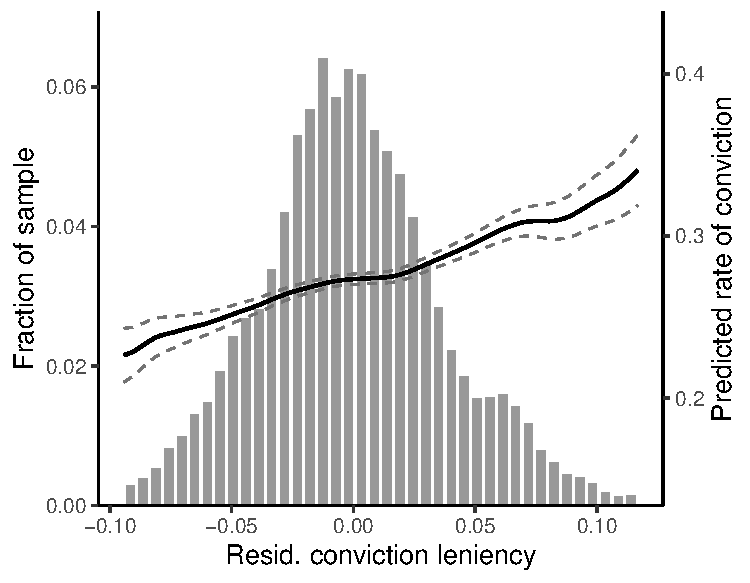
\includegraphics[width=\linewidth]{figures/first_stage_primary_all.pdf}
\caption{All defendants}\label{fig:fs_primary_all}
\end{subfigure}

\begin{subfigure}{0.49\textwidth}
\centering
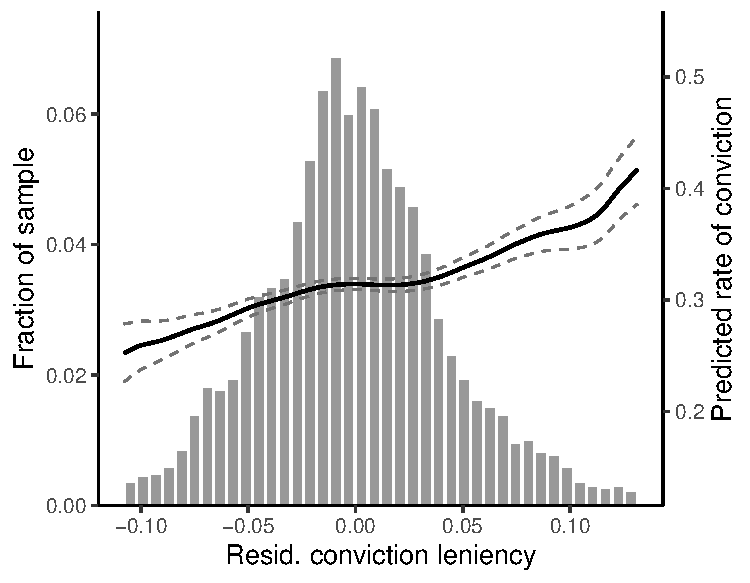
\includegraphics[width=\linewidth]{figures/first_stage_primary_white.pdf}
\caption{White defendants}\label{fig:fs_primary_white}
\end{subfigure}\hfill
\begin{subfigure}{0.49\textwidth}
\centering
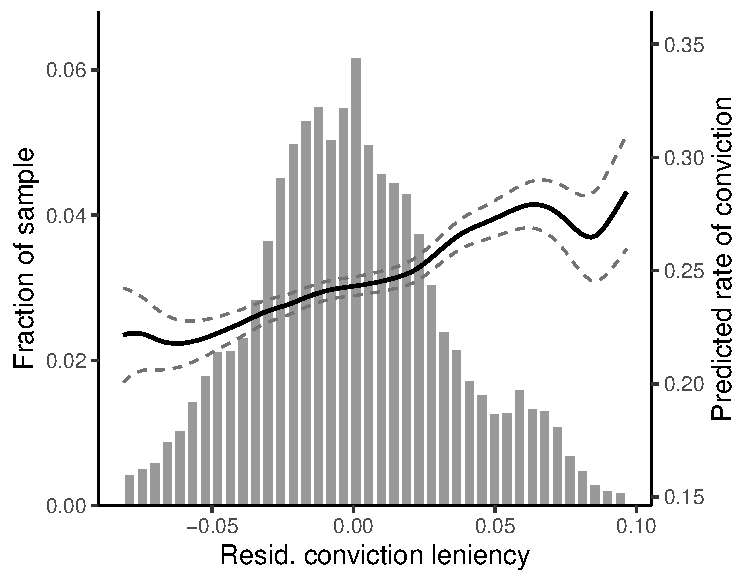
\includegraphics[width=\linewidth]{figures/first_stage_primary_black.pdf}
\caption{Black defendants}\label{fig:fs_primary_black}
\end{subfigure}
\caption{Distribution of conviction leniency and the first stage}\label{fig:fs_primary}
\tabnote{Convicted cases with a matched sentencing score. Histogram (left axis): conviction leniency net of the controls and fixed effects (including the offense group $\times$ score fixed effects, not dismissal leniency), 1st--99th percentiles. Solid line (right axis, predicted rate of non-carceral conviction): local linear regression (Epanechnikov kernel, bandwidth equal to the standard deviation of the instrument; fitted on the 0.1st--99.9th percentiles, shown on the 1st--99th) of non-carceral conviction net of the same controls, plus its mean, on the residualized instrument; dashed lines: 95\% confidence interval, clustered by defendant. \poolnote{} \racesamplenote}
\end{figure}

\begin{figure}[H]
\centering
\begin{subfigure}{0.49\textwidth}
\centering
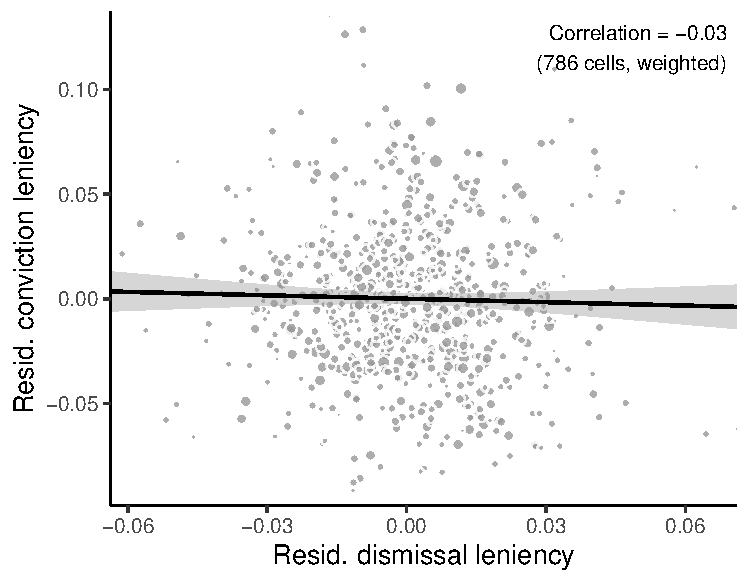
\includegraphics[width=\linewidth]{figures/leniency_scatter_primary_all.pdf}
\caption{All defendants}\label{fig:scatter_all}
\end{subfigure}

\begin{subfigure}{0.49\textwidth}
\centering
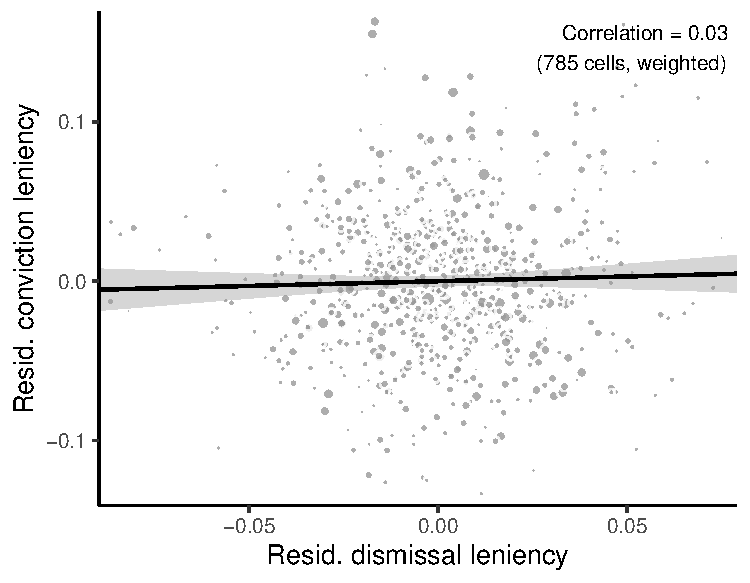
\includegraphics[width=\linewidth]{figures/leniency_scatter_primary_white.pdf}
\caption{White defendants}\label{fig:scatter_white}
\end{subfigure}\hfill
\begin{subfigure}{0.49\textwidth}
\centering
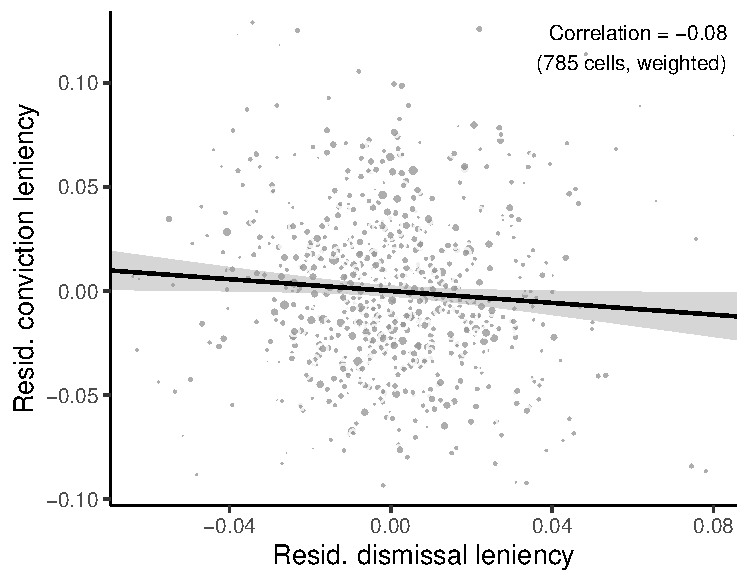
\includegraphics[width=\linewidth]{figures/leniency_scatter_primary_black.pdf}
\caption{Black defendants}\label{fig:scatter_black}
\end{subfigure}
\caption{Conviction leniency against dismissal leniency}\label{fig:scatter}
\tabnote{Each point is a judge $\times$ year $\times$ court cell: conviction leniency (the judge's residualized leave-out non-carceral rate among convicted cases with a matched sentencing score) against dismissal leniency (residualized leave-out dismissal rate over all cases), both net of the controls and fixed effects and averaged over the cell's convicted cases with a matched score of the panel's defendants; point size proportional to the number of cases. \poolnote{} Line: linear fit weighted by cases, with its 95\% confidence interval. Axes show the 0.5th--99.5th percentiles of the cells; the fit and correlation use all cells. \racesamplenote}
\end{figure}

\subsection{Balance}\label{sec:balance}

Table~\ref{tab:balance_primary} regresses non-carceral conviction and conviction leniency on defendant characteristics, with the fixed effects (including the offense group $\times$ score cells) and without dismissal leniency. The characteristics predict non-carceral conviction (joint $F$ between 15 and 37) but not the instrument, which is balanced for White ($F = 0.91$, $p = 0.57$), Black ($F = 0.60$, $p = 0.89$) and all defendants ($F = 0.76$, $p = 0.74$). Of the 34 coefficients on the race-specific instruments, none is significant at 5\% and three at 10\% (White, burglary and traffic; Black, robbery), about what chance produces (1.7 and 3.4 expected).

\begin{table}[H]
\centering
\caption{Balance: non-carceral conviction and conviction leniency}\label{tab:balance_primary}
{\renewcommand{\arraystretch}{0.85}\resizebox{0.85\textwidth}{!}{% Primary instruments. Balance: non-carceral conviction (Conviction) and the conviction instrument
% (loo_d1_cond_jyr_rv_race; Leniency) regressed on the covariates, with fixed effects: court x year,
% court x calendar month, court x day of week, guidelines offense group x sentencing score (one
% indicator per cell). All defendants: White and Black defendants, the fixed effects specific to each
% race. Any misdemeanor charge: in the case. Prior convictions between 31 days and 5 years before
% the case's first offense: felony, a convicted felony case in the full circuit-court record or a
% Sentencing Commission sentencing event of the defendant; misdemeanor only, a convicted misdemeanor
% circuit-court case and no felony conviction. Convicted cases with a matched score only. Standard
% errors clustered by defendant; joint F-test of all covariates. White and Black defendants: only
% the cases of judges with at least 50 convicted cases with a matched score of White and 50 of Black
% defendants in the case's 3-year window.
\begin{tabular}{lcccccc}
\toprule
 & \multicolumn{2}{c}{All} & \multicolumn{2}{c}{White} & \multicolumn{2}{c}{Black} \\
\cmidrule(lr){2-3}\cmidrule(lr){4-5}\cmidrule(lr){6-7}
 & Conviction & Leniency & Conviction & Leniency & Conviction & Leniency \\
 & (1) & (2) & (3) & (4) & (5) & (6) \\
\midrule
Female & $0.0382^{***}$ & $0.0003$ & $0.0333^{***}$ & $0.0007$ & $0.0433^{***}$ & $-0.0001$ \\
 & (0.0038) & (0.0004) & (0.0055) & (0.0006) & (0.0053) & (0.0005) \\
Prior felony conviction (5 years) & $-0.0178^{***}$ & $-0.0004$ & $-0.0140^{***}$ & $-0.0004$ & $-0.0205^{***}$ & $-0.0004$ \\
 & (0.0032) & (0.0004) & (0.0054) & (0.0007) & (0.0039) & (0.0004) \\
Prior misdemeanor only conviction (5 years) & $-0.0185^{***}$ & $-0.0002$ & $0.0000$ & $-0.0006$ & $-0.0334^{***}$ & $0.0002$ \\
 & (0.0066) & (0.0008) & (0.0103) & (0.0013) & (0.0085) & (0.0009) \\
Offense: assault & $-0.0859^{***}$ & $0.0015$ & $-0.0843^{***}$ & $0.0015$ & $-0.0875^{***}$ & $0.0015$ \\
 & (0.0082) & (0.0009) & (0.0160) & (0.0021) & (0.0096) & (0.0010) \\
Offense: burglary & $-0.0528^{***}$ & $0.0012$ & $-0.0795^{***}$ & $0.0029^{*}$ & $-0.0322^{***}$ & $0.0000$ \\
 & (0.0085) & (0.0009) & (0.0138) & (0.0016) & (0.0107) & (0.0011) \\
Offense: drugs & $-0.0447^{***}$ & $-0.0009$ & $-0.0256^{*}$ & $-0.0013$ & $-0.0621^{***}$ & $-0.0006$ \\
 & (0.0088) & (0.0009) & (0.0136) & (0.0015) & (0.0113) & (0.0010) \\
Offense: fraud & $-0.0038$ & $-0.0002$ & $-0.0131$ & $-0.0001$ & $0.0055$ & $-0.0002$ \\
 & (0.0084) & (0.0008) & (0.0119) & (0.0012) & (0.0119) & (0.0011) \\
Offense: kidnapping & $-0.0269^{**}$ & $0.0002$ & $-0.0128$ & $0.0046$ & $-0.0331^{***}$ & $-0.0013$ \\
 & (0.0107) & (0.0017) & (0.0224) & (0.0034) & (0.0119) & (0.0019) \\
Offense: larceny & $-0.0527^{***}$ & $-0.0004$ & $-0.0599^{***}$ & $-0.0005$ & $-0.0467^{***}$ & $-0.0003$ \\
 & (0.0065) & (0.0007) & (0.0103) & (0.0011) & (0.0084) & (0.0008) \\
Offense: miscellaneous & $-0.0066$ & $-0.0008$ & $-0.0205$ & $-0.0007$ & $0.0066$ & $-0.0009$ \\
 & (0.0111) & (0.0012) & (0.0169) & (0.0020) & (0.0147) & (0.0015) \\
Offense: murder & $-0.0195$ & $0.0017$ & $-0.0224$ & $0.0081$ & $-0.0196$ & $0.0003$ \\
 & (0.0240) & (0.0030) & (0.0346) & (0.0070) & (0.0283) & (0.0033) \\
Offense: robbery & $-0.0944^{***}$ & $-0.0019$ & $-0.1565^{***}$ & $0.0002$ & $-0.0717^{***}$ & $-0.0026^{*}$ \\
 & (0.0124) & (0.0013) & (0.0241) & (0.0029) & (0.0143) & (0.0014) \\
Offense: sex assault & $-0.0445^{**}$ & $0.0014$ & $-0.0799^{***}$ & $0.0037$ & $0.0061$ & $-0.0024$ \\
 & (0.0220) & (0.0026) & (0.0295) & (0.0036) & (0.0317) & (0.0035) \\
Offense: sex offense & $-0.0131$ & $-0.0018$ & $-0.0407$ & $-0.0009$ & $0.0256$ & $-0.0027$ \\
 & (0.0218) & (0.0028) & (0.0282) & (0.0037) & (0.0345) & (0.0041) \\
Offense: traffic & $-0.0779^{***}$ & $0.0008$ & $-0.1053^{***}$ & $0.0040^{*}$ & $-0.0632^{***}$ & $-0.0009$ \\
 & (0.0092) & (0.0011) & (0.0160) & (0.0021) & (0.0112) & (0.0012) \\
Offense: weapon & $-0.0597^{***}$ & $-0.0009$ & $-0.0575^{***}$ & $-0.0005$ & $-0.0599^{***}$ & $-0.0011$ \\
 & (0.0066) & (0.0008) & (0.0151) & (0.0019) & (0.0073) & (0.0009) \\
Any misdemeanor charge & $-0.0003$ & $0.0002$ & $-0.0063$ & $0.0004$ & $0.0043$ & $0.0001$ \\
 & (0.0047) & (0.0005) & (0.0074) & (0.0009) & (0.0060) & (0.0006) \\
\midrule
Joint F-statistic & 36.71 & 0.76 & 15.28 & 0.91 & 24.10 & 0.60 \\
Joint F-test p-value & 0.000 & 0.742 & 0.000 & 0.566 & 0.000 & 0.892 \\
Mean of dependent variable & 0.2736 & $-$0.0011 & 0.3131 & $-$0.0010 & 0.2448 & $-$0.0012 \\
Observations & 80,543 & 80,543 & 33,969 & 33,969 & 46,574 & 46,574 \\
\bottomrule
\multicolumn{7}{l}{\footnotesize $^{*}$ p $<$ 0.1, $^{**}$ p $<$ 0.05, $^{***}$ p $<$ 0.01} \\
\end{tabular}
}}
\tabnote{Convicted cases with a matched sentencing score. Columns (1), (3), (5): non-carceral conviction; (2), (4), (6): conviction leniency, each regressed on the covariates with court $\times$ year, court $\times$ calendar month, court $\times$ day-of-week and offense group $\times$ score fixed effects. The instruments are built within the defendant's race; columns (1)--(2) pool White and Black defendants, with the fixed effects specific to each race and common covariate coefficients (as Arnold, Dobbie and Yang 2018). Offense: any felony charge of the case in the code-section group. Any misdemeanor charge: in the focal case. Prior convictions, between 31 days and five years before the focal case's first offense: felony, a convicted felony circuit-court case or a Sentencing Commission sentencing event; misdemeanor only, a convicted misdemeanor circuit-court case and no felony conviction. Joint $F$-statistic and $p$-value: Wald test that all covariate coefficients are zero. Standard errors, in parentheses, clustered by defendant. \racesamplenote}
\end{table}

\subsection{Monotonicity}\label{sec:monotonicity}

Monotonicity requires that a judge who is more lenient toward one kind of defendant is not harsher toward another. Table~\ref{tab:mono_primary} tests it with split samples: conviction leniency is built from one group's cases only (White vs Black defendants, for all defendants only; men vs women; with vs without a prior felony conviction), and its first stage is estimated on the other group, controlling for dismissal leniency built from the same group, as in the 2SLS. All 14 coefficients are positive and significant at 1\% (0.19 to 0.78), for all defendants and within race. They are larger when the instrument comes from the larger group (all defendants: men $\rightarrow$ women 0.598, women $\rightarrow$ men 0.198; Black $\rightarrow$ White 0.783, White $\rightarrow$ Black 0.505), because an instrument built from fewer cases is noisier.

\begin{table}[H]
\centering
\caption{Split-sample monotonicity: first stages}\label{tab:mono_primary}
% Primary instruments. Split-sample monotonicity: for each split, the conviction instrument is
% built from one group only and the first stage of non-carceral conviction on it is estimated on
% the other group, controlling for the dismissal instrument built from the same group; coefficient
% on the conviction instrument and (standard error). Controls and fixed effects as in the first
% stages, without the controls constant within the group; standard errors clustered by defendant.
% The conviction instrument is built from the convicted cases with a matched score of the defendant's
% race (as in the analysis), restricted to the group; the dismissal instrument from all cases of the
% race. All defendants (White and Black): the race split builds the instruments from one race's cases
% and estimates the first stage on the other race; the other splits build each race's instruments
% from that race's cases of the group and estimate the first stage on both races, every control and
% fixed effect specific to each race and one coefficient on each instrument, so the coefficient is a
% weighted average of the White and Black ones. White and Black defendants: only the cases of judges
% with at least 50 convicted cases with a matched score of White and 50 of Black defendants in the
% case's 3-year window.
\begin{tabular}{lccc}
\toprule
Instrument built from $\rightarrow$ first stage on & All & White & Black \\
\midrule
\multicolumn{4}{l}{\textit{Race}} \\
White $\rightarrow$ Black & $0.505^{***}$ &  &  \\
 & (0.037) &  &  \\
Black $\rightarrow$ White & $0.783^{***}$ &  &  \\
 & (0.057) &  &  \\
\addlinespace
\multicolumn{4}{l}{\textit{Sex}} \\
Male $\rightarrow$ Female & $0.598^{***}$ & $0.551^{***}$ & $0.682^{***}$ \\
 & (0.078) & (0.098) & (0.128) \\
Female $\rightarrow$ Male & $0.198^{***}$ & $0.213^{***}$ & $0.188^{***}$ \\
 & (0.021) & (0.035) & (0.027) \\
\addlinespace
\multicolumn{4}{l}{\textit{Prior felony conviction (5 years)}} \\
No prior felony $\rightarrow$ Prior felony & $0.504^{***}$ & $0.555^{***}$ & $0.457^{***}$ \\
 & (0.054) & (0.083) & (0.069) \\
Prior felony $\rightarrow$ No prior felony & $0.302^{***}$ & $0.280^{***}$ & $0.338^{***}$ \\
 & (0.030) & (0.038) & (0.047) \\
\bottomrule
\multicolumn{4}{l}{\footnotesize $^{*}$ p $<$ 0.1, $^{**}$ p $<$ 0.05, $^{***}$ p $<$ 0.01} \\
\end{tabular}

\tabnote{Each coefficient: first stage of non-carceral conviction on conviction leniency built from the cases of one group only (``built from $\rightarrow$ first stage on''), estimated on the cases of the other group, controlling for dismissal leniency built from the same group. The instruments are the residualized leave-out rates of the analysis, built within the defendant's race and restricted to the group, so the defendant's own outcome cannot enter them. All defendants: the race split builds the instrument from one race's cases and estimates the first stage on the other race; the other splits build each race's instrument from that race's cases of the group and estimate the first stage on both races, with every control and fixed effect specific to each race and one coefficient on each instrument. Controls constant within the group are left out. \specnoteprim{} \racesamplenote}
\end{table}

\paragraph{Leniency by race.} Because the instruments are built within race, the 2SLS does not require that a judge who is lenient toward White defendants also be lenient toward Black ones, but the White $-$ Black difference is simplest to interpret if judges rank the same way for both. As far as sampling error lets us tell, they do. Table~\ref{tab:len_race} and Figure~\ref{fig:len_race} compare each judge's leniency toward each race (the mean residualized non-carceral sentence of the judge's cases of that race) over each three-year window (756 judge-windows), relative to the other judges of the same court and center year, as the instrument compares them. The raw correlation is 0.61. With reliabilities of 0.60 and 0.59, identical true leniencies would show a correlation of only about $\sqrt{0.60 \times 0.59} = 0.59$; corrected for sampling error with random halves of each judge's defendants, each residualized in its own regression,\footnote{In one regression, the residuals of cases that share a fixed-effect cell are negatively correlated (their covariance is $-\sigma^2 h_{jk}$, with $h_{jk}$ the off-diagonal element of the hat matrix), which would make two halves of the same race disagree by more than sampling error and understate the reliability; with both halves in one regression, the corrected correlation comes out at about 1.3. The split-half reliability of the instrument (Appendix~\ref{sec:f_details}) is not affected (0.61 and 0.60 either way), because it compares the halves net of the court-year fixed effects, which absorb a shift common to the cases of a court-year.} the correlation is 1.03 (95\% bootstrap interval over judges: 0.91 to 1.15; a corrected correlation can exceed 1 by sampling error when the true one is close to 1: Charles 2005). Of the 1,403 pairs of judges in the same court and window year, 69\% are ranked the same way by White and by Black leniency; in random halves, a pair is ranked the same way across races (63\%) at least as often as across two halves of the same race (62\%), whose disagreements are sampling error alone. A regression of a judge-window's percentile rank in White leniency on that in Black leniency gives 0.51 (s.e.\ 0.03), against 0.83 in Arnold, Dobbie and Yang (2018); ranks are attenuated by sampling error like correlations, and our judge-windows rest on far fewer cases (medians of 110 White and 150 Black cases, against 179 to 5,253 cases of all races per judge-year cell in theirs).

\begin{table}[H]
\centering
\caption{Judges' leniency toward White and Black defendants}\label{tab:len_race}
{\small% Primary analysis. Leniency of a judge toward a race: mean residualized non-carceral sentence
% (the first-step residual of the race-specific instrument) over the judge's convicted cases with a
% matched score of that race in the race samples, per judge x court over the 3-year window centered
% on each year with cases (the cases the instrument averages), relative to the other judges of the
% same court and center year, the comparisons the instrument makes: minus the group's mean weighted
% by the smaller of the two case counts, judge-windows without another judge in their group dropped.
% Correlation weighted by the smaller of the two case counts. Reliability: Spearman-Brown from random
% halves of the judge's defendants, each residualized in its own regression (20 splits); corrected
% correlation: correlation between a White and a Black half over the square root of the product of
% the correlations between the two halves of each race (the halves' leniency relative to the group
% likewise); in brackets, its 95% interval from 1000 bootstrap draws of judges (the splits' half means
% kept). Rank regression: percentile rank (across judge-windows) in White leniency on percentile rank
% in Black leniency, unweighted. Pairs: judges in the same court and window year; same ordering: share
% of pairs ranked the same way.
\begin{tabular}{lc}
\toprule
 & Judge $\times$ 3-year window \\
\midrule
Units & 756 \\
Median cases per unit, White & 110 \\
Median cases per unit, Black & 150 \\
\addlinespace
Correlation of White and Black leniency & 0.61 \\
Reliability of White leniency & 0.60 \\
Reliability of Black leniency & 0.59 \\
Correlation corrected for sampling error & 1.03 \\
 & [0.91, 1.15] \\
Rank regression, White on Black & 0.512 \\
 & (0.031) \\
\addlinespace
Pairs of judges compared & 1,403 \\
Same ordering by White and Black leniency & 0.69 \\
Same ordering in random halves: White vs Black & 0.63 \\
Same ordering in random halves: same race & 0.62 \\
\bottomrule
\end{tabular}
}
\tabnote{Leniency of a judge toward a race: the mean residualized non-carceral sentence (the first-step residual the race-specific instrument averages) over the judge's convicted cases with a matched score of that race, per judge and court over the three-year window centered on each year with cases (the cases the instrument averages, without the leave-out), relative to the other judges of the same court and center year: the judge's mean minus the group's mean weighted by the smaller of the two case counts; judge-windows without a colleague in their group are left out. Correlation weighted by the smaller of the two case counts. Reliability: $2r/(1+r)$, with $r$ the correlation between random halves of the judge's defendants, each half residualized in its own regression, averaged over 20 splits; corrected correlation: the correlation between a White and a Black half divided by the square root of the product of the correlations between the two halves of each race (the halves' leniency also relative to the group); in brackets, its 95\% interval from 1,000 bootstrap draws of judges, the splits' half means kept. Rank regression: percentile rank, across judge-windows, of the leniency relative to the group, White on Black, unweighted (standard error in parentheses). Pairs: judges in the same court and window year; same ordering: the share of pairs ranked the same way; in random halves, across races (one race's half against the other race's) and within race (the two halves of the same race). \racesamplenote}
\end{table}

\begin{figure}[H]
\centering
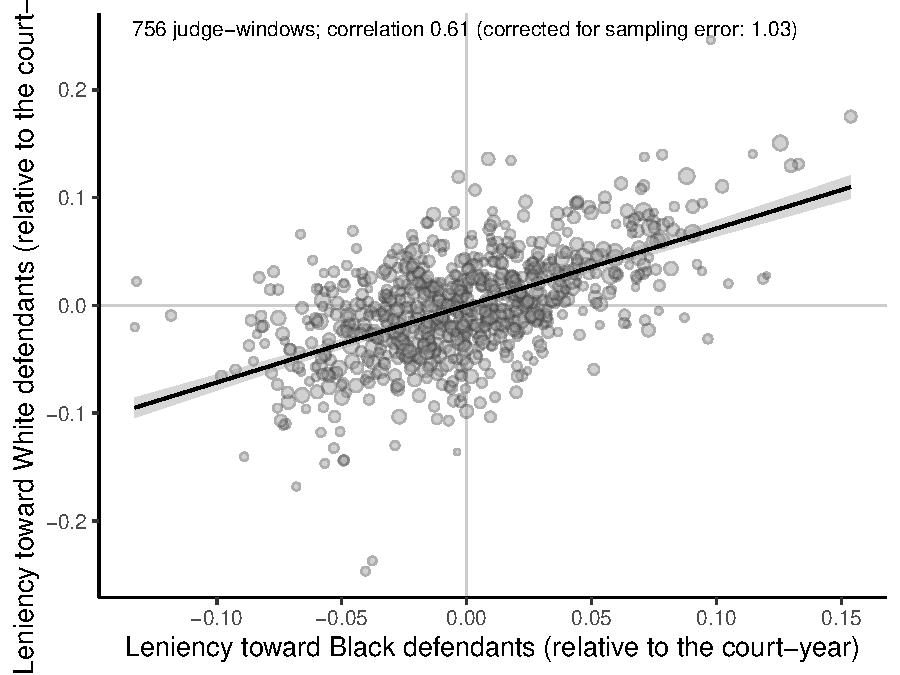
\includegraphics[width=0.7\textwidth]{figures/leniency_by_race_primary.pdf}
\caption{Judges' leniency toward White and Black defendants}\label{fig:len_race}
\tabnote{Each point is a judge-window (a judge's cases in a court over the three-year window centered on a year): the mean residualized non-carceral sentence of the judge's convicted cases with a matched score of White defendants against that of Black defendants, each relative to the other judges of the same court and center year; point size proportional to the judge-window's cases. Line: linear fit weighted by the smaller of the two case counts, with its 95\% confidence interval. \racesamplenote}
\end{figure}

\subsection{The revocation measures and the exclusion restriction}\label{sec:exclusion}

The judge can affect revocations other than through the choice of a non-carceral sentence: through the conditions of the sentence (the length of probation and of the suspended sentence, supervision, special conditions), which affect the risk of a violation, and through the revocation decision itself. Such a channel violates the exclusion restriction only if it is correlated with the judge's leniency (``average exclusion'': Frandsen, Lefgren and Leslie 2023; Chyn, Frandsen and Leslie 2025). Three pieces of evidence bear on it and motivate the choice of the primary measure.

\emph{Who decides.} Table~\ref{tab:rev_judges} compares, for each kind of revocation proceeding and for new felony cases, the share decided by the focal case's judge with the share expected if the deciding judge were drawn in proportion to the judges' caseloads in the court and year. The focal judge decides 64\% of the proceedings on the focal sentences (21\% at random), but only 17\% of those of the primary measure (12\% at random), little more than the 14\% of new felony cases (11\%). The primary measure is therefore barely exposed to the focal judge's revocation decisions, and the conditions of its sentences were set at other hearings, mostly by other judges; the secondary measure is exposed to both. (The focal judge decides 19\% of the proceedings counted in neither measure, 13\% at random.)

\emph{Proceedings are not filed by the judge.} A proceeding is initiated by the probation officer's violation report or the prosecutor's motion; the judge decides only whether to revoke. Effects on proceedings are therefore less exposed than effects on revocations, though not entirely: a defendant who expects the same lenient judge might violate more readily, which would affect every outcome.

\emph{Judges' revocation decisions are only weakly related to their sentencing leniency.} The concern is that a judge who sentences leniently also revokes leniently, which would turn the focal judge's deciding most revocations of the focal sentences into an exclusion violation. Table~\ref{tab:rev_decisions} uses the felony revocation proceedings of White and Black defendants filed in 2000--2019 before a judge who also sentences analysis cases of the defendant's race that year (45,635 and 73,742 proceedings). Separately by race, it regresses whether the sentence was \emph{not} revoked (14.2\% and 13.4\% of proceedings) on the deciding judge's leniency toward the defendant's race, measured from that judge's own sentencing that year (the mean of the race-specific instrument over the analysis cases of that race the judge sentences), with court $\times$ year fixed effects. The coefficient per unit of conviction leniency is 0.043 (s.e.\ 0.035) for White and 0.049 (0.051) for Black defendants, and 0.042 (0.033) and 0.055 (0.050) holding dismissal leniency fixed, none significant: one standard deviation of leniency within court and year (0.051 and 0.041) keeps 0.2 points more sentences in both groups. Taken at face value, this would lower the effect on the focal sentences being revoked by about 0.02 for both groups (the share of these proceedings decided by the focal judge, 0.64, times the share of defendants with one, about 0.3, times the coefficient, divided by the first stage, 0.47 and 0.44), against estimates of 0.36 (White) and 0.66 (Black) within three years. Judges who dismiss more do keep more sentences (0.13, s.e.\ 0.08, for White and 0.27, s.e.\ 0.07, for Black defendants, per unit of dismissal leniency), but the 2SLS holds dismissal leniency fixed.

\begin{table}[H]
\centering
\caption{Who decides the defendants' revocation proceedings and new felony cases}\label{tab:rev_judges}
{\small\setlength{\tabcolsep}{4pt}\renewcommand{\arraystretch}{0.9}\resizebox{\textwidth}{!}{% Primary analysis. White and Black defendants of the race samples, cases first disposed in or before
% 2016: their felony revocation proceedings (charges of a case filed on one date) filed within 3 years
% after the focal disposition, by the revocation measure that counts them and the case they are filed
% under, and their new felony cases (judge-IV cases) charged within 3 years. N: proceedings (cases)
% with judge information on their pleadings. Focal judge: share decided by the focal case's judge.
% At random: share expected if the deciding judge were drawn in proportion to the judges' caseloads
% in the court and year (all felony revocation proceedings, or all judge-IV cases), zero in another
% court.
\begin{tabular}{lccc}
\toprule
 & N & Focal judge (\%) & At random (\%) \\
\midrule
\multicolumn{4}{l}{\textit{Counted in the primary revocation measure (other sentences)}} \\
\quad Revocation proceedings: later sentences & 3,050 & 16 & 11 \\
\quad Revocation proceedings: earlier sentences, after a new case & 2,046 & 17 & 12 \\
\quad Revocation proceedings: revocation-only case nos., after a new case & 608 & 26 & 19 \\
\quad Revocation proceedings: all of the primary measure & 5,704 & 17 & 12 \\
\addlinespace
\multicolumn{4}{l}{\textit{Counted in the secondary revocation measure (focal sentences)}} \\
\quad Revocation proceedings: filed under the focal case & 21,872 & 64 & 21 \\
\quad Revocation proceedings: other cases sentenced at the focal hearing & 2,153 & 58 & 22 \\
\quad Revocation proceedings: all of the secondary measure & 24,025 & 64 & 21 \\
\addlinespace
\multicolumn{4}{l}{\textit{Counted in neither revocation measure}} \\
\quad Revocation proceedings: earlier or unidentified, no new case & 9,147 & 19 & 14 \\
\addlinespace
\multicolumn{4}{l}{\textit{Not revocation proceedings}} \\
\quad New felony cases (not revocation proceedings) & 17,680 & 14 & 11 \\
\bottomrule
\end{tabular}
}}
\tabnote{White and Black defendants of the race samples, cases first disposed in or before 2016: their felony revocation proceedings (the charges of a case filed on one date) filed within three years after the focal disposition, grouped by the measure that counts them and the case they are filed under, and their new felony cases (judge-IV cases) charged within three years. N: proceedings (cases) with judge information on their pleadings. Focal judge: the share decided by the focal case's judge. At random: the share expected if the deciding judge were drawn in proportion to the judges' caseloads in the court and year (all felony revocation proceedings, or all judge-IV cases), zero in another court. \racesamplenote}
\end{table}

\begin{table}[H]
\centering
\caption{Revocation decisions and the deciding judge's sentencing leniency}\label{tab:rev_decisions}
{\small\renewcommand{\arraystretch}{0.9}\resizebox{\textwidth}{!}{% Felony revocation proceedings of White (columns 1-2) and Black (columns 3-4) defendants filed
% 2000-2019 before a judge of the analysis in a year in which the judge also sentences analysis cases
% of the defendant's race. Dependent variable: not revoked (no charge of the proceeding ends with
% the sentence revoked or the violation found). Regressors: the leniency of the judge deciding the
% proceeding (not of the judge who imposed the revoked sentence) toward the defendant's race, measured
% by their sentencing decisions: their mean race-specific instrument of the primary analysis in the
% year over the analysis cases of that race they sentence (conviction leniency: over convicted cases
% with a matched score; dismissal leniency: over all cases). Court x year fixed effects; standard
% errors, in parentheses, clustered by judge.
\begin{tabular}{lcccc}
\toprule
 & \multicolumn{2}{c}{White defendants} & \multicolumn{2}{c}{Black defendants} \\
\cmidrule(lr){2-3}\cmidrule(lr){4-5}
 & (1) & (2) & (3) & (4) \\
\midrule
Deciding judge's conviction leniency & $0.043$ & $0.042$ & $0.049$ & $0.055$ \\
 & (0.035) & (0.033) & (0.051) & (0.050) \\
Deciding judge's dismissal leniency &  & $0.131$ &  & $0.266^{***}$ \\
 &  & (0.082) &  & (0.071) \\
\midrule
SD of conviction leniency within court $\times$ year & 0.051 & 0.051 & 0.041 & 0.041 \\
Mean of not revoked & 0.142 & 0.142 & 0.134 & 0.134 \\
Proceedings & 45,635 & 45,635 & 73,742 & 73,742 \\
Judges & 177 & 177 & 179 & 179 \\
\bottomrule
\multicolumn{5}{l}{\footnotesize $^{*}$ p $<$ 0.1, $^{**}$ p $<$ 0.05, $^{***}$ p $<$ 0.01} \\
\end{tabular}
}}
\tabnote{Unit: a felony revocation proceeding of a White (columns 1--2) or Black (columns 3--4) defendant filed in 2000--2019 before a judge of the analysis in a year in which the judge also sentences analysis cases of the defendant's race. Dependent variable: not revoked (no charge of the proceeding ends with the sentence revoked or the violation found). Regressors: the leniency of the judge deciding the proceeding (not of the judge who imposed the revoked sentence) toward the defendant's race, measured from that judge's sentencing: the mean, over the analysis cases of that race the judge sentences that year, of this report's race-specific conviction leniency (over convicted cases with a matched score) and dismissal leniency (over all cases). Court $\times$ year fixed effects; standard errors, in parentheses, clustered by judge.}
\end{table}

\subsection{Recidivism and sentence lengths of incarcerated defendants}\label{sec:base_recid}

Among incarcerated defendants, recidivism is similar by race (Table~\ref{tab:recid_inc}; cases disposed by 2016): within three years of the disposition, 21.7\% of White and 21.4\% of Black defendants are charged with a new felony case, 9.1\% and 6.9\% have a revocation proceeding on another sentence, and 29.8\% and 27.2\% one on the focal sentences. Within three years of release (Table~\ref{tab:recid_inc_rel}; cases disposed by 2012), the shares are 24.7\% and 27.2\%, 11.3\% and 10.4\%, and 32.3\% and 32.7\%.

Sentences are longer for Black defendants (Figure~\ref{fig:sentence_length}): the mean active carceral time is 1.29 years for White and 1.95 years for Black defendants (medians 0.67 and 1.00); 44\% and 57\% are sentenced to a year or more, 11\% and 20\% to three years or more, and 5\% and 11\% to five years or more. A year after the disposition, 29\% and 41\% are still in custody (8\% and 15\% after three years). A window that starts at the disposition therefore removes more of the time at risk of incarcerated Black defendants, one reason to measure the outcomes from release as well.

\begin{figure}[H]
\centering
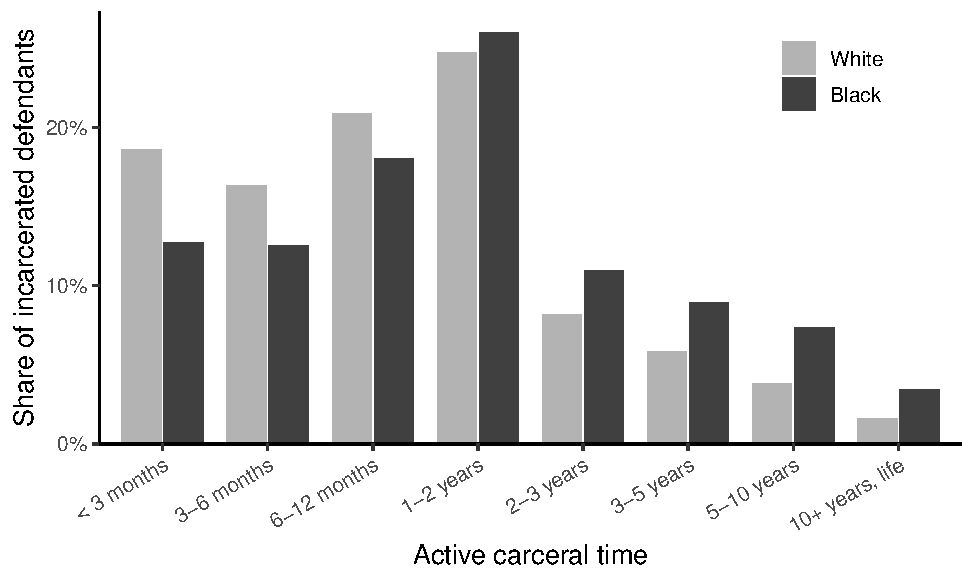
\includegraphics[width=0.8\textwidth]{figures/sentence_length_primary.pdf}
\caption{Active carceral time of incarcerated defendants, by race}\label{fig:sentence_length}
\tabnote{Incarcerated defendants (carceral sentence in the focal case) of the race samples, convicted cases with a matched sentencing score first disposed in or before 2016 (20,059 White and 31,397 Black defendants; the cases of the 2SLS from the disposition): share of each race's incarcerated defendants by active carceral time, the jail and penitentiary time net of the suspended part, with the case's sentences consecutive unless the court made them concurrent. Bins include their lower bound. \racesamplenote}
\end{figure}

\begin{table}[H]
\centering
\caption{Recidivism of incarcerated defendants from the disposition, by race}\label{tab:recid_inc}
\resizebox{\textwidth}{!}{% Primary instruments' sample. Share of incarcerated defendants (d2 = 1, convicted cases with a
% matched score) with any new felony CC case charged / convicted / incarcerated, any revocation
% proceeding / revocation of the person's other felony sentences, or of the focal felony sentences
% (04), within 1, 2 and 3 years after the case's first disposition; all outcomes on the cases first
% disposed in or before 2016 (full follow-up for 3 years in the circuit-court record, which ends in
% 2019). Stars: test that the share is zero; standard errors, in parentheses, clustered by person.
% White and Black defendants: only the cases of judges with at least 50 convicted cases with a matched
% score of White and 50 of Black defendants in the case's 3-year window.
\begin{tabular}{lcccccc}
\toprule
 & \multicolumn{2}{c}{1 year} & \multicolumn{2}{c}{2 years} & \multicolumn{2}{c}{3 years} \\
\cmidrule(lr){2-3}\cmidrule(lr){4-5}\cmidrule(lr){6-7}
 & White & Black & White & Black & White & Black \\
\midrule
\multicolumn{7}{l}{\textit{New felony CC case}} \\
Charged & $0.073^{***}$ & $0.066^{***}$ & $0.151^{***}$ & $0.145^{***}$ & $0.217^{***}$ & $0.214^{***}$ \\
 & (0.002) & (0.001) & (0.003) & (0.002) & (0.003) & (0.002) \\
Convicted & $0.068^{***}$ & $0.059^{***}$ & $0.141^{***}$ & $0.131^{***}$ & $0.202^{***}$ & $0.194^{***}$ \\
 & (0.002) & (0.001) & (0.003) & (0.002) & (0.003) & (0.002) \\
Incarcerated & $0.057^{***}$ & $0.051^{***}$ & $0.117^{***}$ & $0.113^{***}$ & $0.169^{***}$ & $0.169^{***}$ \\
 & (0.002) & (0.001) & (0.002) & (0.002) & (0.003) & (0.002) \\
\addlinespace
\multicolumn{7}{l}{\textit{Revocation of the person's other sentences}} \\
Proceeding & $0.015^{***}$ & $0.010^{***}$ & $0.051^{***}$ & $0.036^{***}$ & $0.091^{***}$ & $0.069^{***}$ \\
 & (0.001) & (0.001) & (0.002) & (0.001) & (0.002) & (0.002) \\
Revoked & $0.013^{***}$ & $0.009^{***}$ & $0.047^{***}$ & $0.032^{***}$ & $0.084^{***}$ & $0.062^{***}$ \\
 & (0.001) & (0.001) & (0.002) & (0.001) & (0.002) & (0.001) \\
\addlinespace
\multicolumn{7}{l}{\textit{Revocation of the focal sentences}} \\
Proceeding & $0.102^{***}$ & $0.085^{***}$ & $0.221^{***}$ & $0.192^{***}$ & $0.298^{***}$ & $0.272^{***}$ \\
 & (0.002) & (0.002) & (0.003) & (0.002) & (0.003) & (0.003) \\
Revoked & $0.089^{***}$ & $0.075^{***}$ & $0.198^{***}$ & $0.172^{***}$ & $0.267^{***}$ & $0.243^{***}$ \\
 & (0.002) & (0.002) & (0.003) & (0.002) & (0.003) & (0.003) \\
\midrule
Incarcerated defendants (cases) & 20,059 & 31,397 & 20,059 & 31,397 & 20,059 & 31,397 \\
\bottomrule
\multicolumn{7}{l}{\footnotesize $^{*}$ p $<$ 0.1, $^{**}$ p $<$ 0.05, $^{***}$ p $<$ 0.01} \\
\end{tabular}
}
\tabnote{Share of incarcerated defendants (carceral sentence in the focal case; convicted cases with a matched sentencing score) with the outcome within 1, 2 or 3 years after the focal case's first disposition, all on the cases first disposed in or before 2016 (full follow-up for three years). Revocations: the primary measure (the person's other sentences) and the secondary one (the focal sentences; Section~\ref{sec:data}). Stars: test that the share is zero; standard errors, in parentheses, clustered by person. \racesamplenote}
\end{table}

\begin{table}[H]
\centering
\caption{Recidivism of incarcerated defendants from release, by race}\label{tab:recid_inc_rel}
\resizebox{\textwidth}{!}{% Primary instruments' sample. Share of incarcerated defendants (d2 = 1, convicted cases with a
% matched score) with any new felony CC case charged / convicted / incarcerated, any revocation
% proceeding / revocation of the person's other felony sentences, or of the focal felony sentences
% (04), within 1, 2 and 3 years after release from the focal sentence (first disposition plus 0.9 x
% active carceral time, at most 4 years); all outcomes on the cases first disposed in or before 2012
% (full follow-up for 3 years in the circuit-court record, which ends in 2019). Stars: test that the
% share is zero; standard errors, in parentheses, clustered by person. White and Black defendants:
% only the cases of judges with at least 50 convicted cases with a matched score of White and 50 of
% Black defendants in the case's 3-year window.
\begin{tabular}{lcccccc}
\toprule
 & \multicolumn{2}{c}{1 year} & \multicolumn{2}{c}{2 years} & \multicolumn{2}{c}{3 years} \\
\cmidrule(lr){2-3}\cmidrule(lr){4-5}\cmidrule(lr){6-7}
 & White & Black & White & Black & White & Black \\
\midrule
\multicolumn{7}{l}{\textit{New felony CC case}} \\
Charged & $0.105^{***}$ & $0.112^{***}$ & $0.186^{***}$ & $0.202^{***}$ & $0.247^{***}$ & $0.272^{***}$ \\
 & (0.003) & (0.002) & (0.004) & (0.003) & (0.004) & (0.003) \\
Convicted & $0.098^{***}$ & $0.100^{***}$ & $0.173^{***}$ & $0.182^{***}$ & $0.231^{***}$ & $0.248^{***}$ \\
 & (0.003) & (0.002) & (0.004) & (0.003) & (0.004) & (0.003) \\
Incarcerated & $0.082^{***}$ & $0.087^{***}$ & $0.144^{***}$ & $0.158^{***}$ & $0.195^{***}$ & $0.216^{***}$ \\
 & (0.003) & (0.002) & (0.003) & (0.003) & (0.004) & (0.003) \\
\addlinespace
\multicolumn{7}{l}{\textit{Revocation of the person's other sentences}} \\
Proceeding & $0.026^{***}$ & $0.025^{***}$ & $0.072^{***}$ & $0.062^{***}$ & $0.113^{***}$ & $0.104^{***}$ \\
 & (0.001) & (0.001) & (0.002) & (0.002) & (0.003) & (0.002) \\
Revoked & $0.023^{***}$ & $0.022^{***}$ & $0.067^{***}$ & $0.056^{***}$ & $0.106^{***}$ & $0.095^{***}$ \\
 & (0.001) & (0.001) & (0.002) & (0.002) & (0.003) & (0.002) \\
\addlinespace
\multicolumn{7}{l}{\textit{Revocation of the focal sentences}} \\
Proceeding & $0.152^{***}$ & $0.154^{***}$ & $0.262^{***}$ & $0.263^{***}$ & $0.323^{***}$ & $0.327^{***}$ \\
 & (0.003) & (0.003) & (0.004) & (0.003) & (0.004) & (0.003) \\
Revoked & $0.136^{***}$ & $0.140^{***}$ & $0.238^{***}$ & $0.240^{***}$ & $0.295^{***}$ & $0.297^{***}$ \\
 & (0.003) & (0.002) & (0.004) & (0.003) & (0.004) & (0.003) \\
\midrule
Incarcerated defendants (cases) & 13,199 & 21,615 & 13,199 & 21,615 & 13,199 & 21,615 \\
\bottomrule
\multicolumn{7}{l}{\footnotesize $^{*}$ p $<$ 0.1, $^{**}$ p $<$ 0.05, $^{***}$ p $<$ 0.01} \\
\end{tabular}
}
\tabnote{As in Table~\ref{tab:recid_inc}, with the outcomes within 1, 2 or 3 years after release from the focal sentence (the first disposition plus 90\% of the active carceral time, at most four years), on the cases first disposed in or before 2012.}
\end{table}

\section{Effects of non-carceral conviction on recidivism}\label{sec:results}

\subsection{Measured from the disposition}\label{sec:disposition}

\paragraph{New felony cases.} Within one year of the disposition, a non-carceral rather than a carceral sentence raises new felony cases for Black defendants, by 0.22 on being charged (s.e.\ 0.09; mean 0.07), 0.21 on being convicted and 0.17 on being incarcerated, all significant at 5\%, and not for White defendants ($-0.02$, 0.06 and $-0.01$; Table~\ref{tab:iv_primary_new}). The differences, $-0.24$ (s.e.\ 0.12), $-0.16$ (0.11) and $-0.17$ (0.10), are significant at 5\% for being charged and at 10\% for being incarcerated. The Black effect fades (0.15 within two years and 0.10 within three, standard errors 0.11 and 0.13), the White estimates rise insignificantly (0.07 and 0.14), and no difference within two or three years is significant. The one-year Black effect is what incapacitation alone would produce: the implied one-year new-charge rate of Black compliers had they been incarcerated is $-0.06$ (s.e.\ 0.07; zero within sampling error), against 0.16 had they not, because incarcerated compliers spend part of the year in custody; measured from release the two rates are about equal (Section~\ref{sec:release}).

\paragraph{Revocations of other sentences} (the primary measure) rise within three years by 0.20 for White (s.e.\ 0.09, significant at 5\%) and 0.03 for Black defendants (s.e.\ 0.08; means 0.10 and 0.07), almost all of it in the second and third years (one year: 0.01 and 0.02; Table~\ref{tab:iv_primary_revo}); the estimates for being revoked are about the same (0.20 and 0.02). The racial difference is significant at 10\% within two years (0.16, s.e.\ 0.09) but not within three (0.17, s.e.\ 0.12). By the sentence revoked (Table~\ref{tab:rev_parts}), most of the effect is on \emph{later sentences}, imposed after the focal disposition (White 0.15, s.e.\ 0.07; Black 0.04, s.e.\ 0.06, within three years), and little on earlier or unidentified sentences counted after a new case (0.06 and $-0.01$). A later sentence exists only if the defendant is sentenced in another case; Section~\ref{sec:revother_meaning} examines what that implies.

\paragraph{Revocations of the focal sentences} (the secondary measure) rise for both groups from the first year (Table~\ref{tab:iv_primary_revf}): by 0.33 (s.e.\ 0.10) for White and 0.42 (0.10) for Black defendants within one year, and by 0.38 (0.14) and 0.64 (0.15) within three. No racial difference is significant (three years: $-0.27$, s.e.\ 0.21). Nearly all of it is on the focal case itself; the other cases sentenced at the focal hearing add 0.14 (White, s.e.\ 0.07) and 0.09 (Black, 0.06) within three years. Had they been incarcerated, compliers would have had a proceeding on these sentences within three years at a rate of 0.081 (White) and 0.045 (Black), against 0.457 and 0.687 under a non-carceral sentence, consistent with placing defendants under supervision from the start.

\begin{table}[H]
\centering
\caption{2SLS from the disposition: non-carceral conviction and new felony cases}\label{tab:iv_primary_new}
{\small\linespread{1}\selectfont\renewcommand{\arraystretch}{0.9}% Primary instruments. 2SLS of any new felony CC case within 1, 2 and 3 years after the case's
% first disposition on non-carceral conviction, instrumented by the conviction instrument
% (loo_d1_cond_jyr_rv_race), controlling for the dismissal instrument (loo_d0_jyr_race), built within
% the defendant's race. Rows: outcomes; columns: White and Black defendants and White minus Black.
% Standard errors in parentheses; outcome mean among the column's defendants in brackets. White minus
% Black: from one regression of White and Black defendants with all controls, fixed effects, the
% treatment and the instrument interacted with a White indicator. Controls: any_assault, any_burglary,
% any_drugs, any_fraud, any_kidnapping, any_larceny, any_miscellaneous, any_murder, any_robbery,
% any_sex_assault, any_sex_offense, any_traffic, any_weapon, any_mis, flag_prior_fel_conv,
% flag_prior_mis_only_conv, female (as fixed effects); fixed effects: court x year, court x calendar
% month, court x day of week, guidelines offense group x sentencing score (one indicator per cell).
% Convicted cases with a matched score only. Standard errors clustered by defendant. All outcomes
% on the same cases, first disposed in or before 2016 (full follow-up for every window in the
% circuit-court record, which ends in 2019). White and Black defendants: only the cases of judges with
% at least 50 convicted cases with a matched score of White and 50 of Black defendants in the case's
% 3-year window.
\begin{tabular}{lccc}
\toprule
 & White & Black & White $-$ Black \\
\midrule
\multicolumn{4}{l}{\textit{Charged}} \\
\quad 1 year & $-0.020$ & $0.218^{**}$ & $-0.238^{**}$ \\
 & (0.082) & (0.085) & (0.118) \\
 & [0.083] & [0.074] &  \\
\quad 2 years & $0.066$ & $0.149$ & $-0.083$ \\
 & (0.107) & (0.114) & (0.156) \\
 & [0.159] & [0.153] &  \\
\quad 3 years & $0.139$ & $0.100$ & $0.040$ \\
 & (0.122) & (0.130) & (0.178) \\
 & [0.221] & [0.219] &  \\
\addlinespace
\multicolumn{4}{l}{\textit{Convicted}} \\
\quad 1 year & $0.057$ & $0.213^{***}$ & $-0.157$ \\
 & (0.079) & (0.081) & (0.113) \\
 & [0.076] & [0.066] &  \\
\quad 2 years & $0.138$ & $0.161$ & $-0.023$ \\
 & (0.104) & (0.110) & (0.152) \\
 & [0.147] & [0.138] &  \\
\quad 3 years & $0.172$ & $0.099$ & $0.073$ \\
 & (0.119) & (0.126) & (0.174) \\
 & [0.205] & [0.199] &  \\
\addlinespace
\multicolumn{4}{l}{\textit{Incarcerated}} \\
\quad 1 year & $-0.008$ & $0.166^{**}$ & $-0.174^{*}$ \\
 & (0.069) & (0.074) & (0.101) \\
 & [0.060] & [0.056] &  \\
\quad 2 years & $0.072$ & $0.095$ & $-0.023$ \\
 & (0.093) & (0.102) & (0.138) \\
 & [0.118] & [0.117] &  \\
\quad 3 years & $0.087$ & $0.025$ & $0.062$ \\
 & (0.109) & (0.119) & (0.161) \\
 & [0.167] & [0.169] &  \\
\midrule
Observations & 29,397 & 41,655 &  \\
\bottomrule
\multicolumn{4}{l}{\footnotesize $^{*}$ p $<$ 0.1, $^{**}$ p $<$ 0.05, $^{***}$ p $<$ 0.01} \\
\end{tabular}
}
\tabnote{Outcomes: any new felony circuit-court case charged, convicted or incarcerated with a case date (first offense, else arrest, hearing, disposition or filing date) within 1, 2 or 3 years after the focal case's first disposition; all windows on the cases first disposed in or before 2016 (full follow-up for three years). \ivnote{} \specnoteprim}
\end{table}

\begin{table}[H]
\centering
\caption{2SLS from the disposition: non-carceral conviction and revocations of other sentences (primary revocation measure)}\label{tab:iv_primary_revo}
{\small\linespread{1}\selectfont\renewcommand{\arraystretch}{0.9}% Primary instruments. 2SLS of any revocation of the person's other felony sentences set off after
% the case's first disposition (sentences imposed after the day of the case's first disposition;
% earlier or unidentified ones only after a new case) within 1, 2 and 3 years after the case's
% first disposition on non-carceral conviction, instrumented by the conviction instrument
% (loo_d1_cond_jyr_rv_race), controlling for the dismissal instrument (loo_d0_jyr_race), built within
% the defendant's race. Rows: outcomes; columns: White and Black defendants and White minus Black.
% Standard errors in parentheses; outcome mean among the column's defendants in brackets. White minus
% Black: from one regression of White and Black defendants with all controls, fixed effects, the
% treatment and the instrument interacted with a White indicator. Controls: any_assault, any_burglary,
% any_drugs, any_fraud, any_kidnapping, any_larceny, any_miscellaneous, any_murder, any_robbery,
% any_sex_assault, any_sex_offense, any_traffic, any_weapon, any_mis, flag_prior_fel_conv,
% flag_prior_mis_only_conv, female (as fixed effects); fixed effects: court x year, court x calendar
% month, court x day of week, guidelines offense group x sentencing score (one indicator per cell).
% Convicted cases with a matched score only. Standard errors clustered by defendant. All outcomes
% on the same cases, first disposed in or before 2016 (full follow-up for every window in the
% circuit-court record, which ends in 2019). White and Black defendants: only the cases of judges with
% at least 50 convicted cases with a matched score of White and 50 of Black defendants in the case's
% 3-year window.
\begin{tabular}{lccc}
\toprule
 & White & Black & White $-$ Black \\
\midrule
\multicolumn{4}{l}{\textit{Proceeding}} \\
\quad 1 year & $0.014$ & $0.024$ & $-0.009$ \\
 & (0.039) & (0.035) & (0.053) \\
 & [0.018] & [0.012] &  \\
\quad 2 years & $0.158^{**}$ & $-0.003$ & $0.162^{*}$ \\
 & (0.070) & (0.060) & (0.092) \\
 & [0.057] & [0.038] &  \\
\quad 3 years & $0.198^{**}$ & $0.029$ & $0.169$ \\
 & (0.089) & (0.081) & (0.120) \\
 & [0.096] & [0.071] &  \\
\addlinespace
\multicolumn{4}{l}{\textit{Revoked}} \\
\quad 1 year & $0.022$ & $0.017$ & $0.005$ \\
 & (0.037) & (0.033) & (0.050) \\
 & [0.016] & [0.010] &  \\
\quad 2 years & $0.161^{**}$ & $-0.004$ & $0.165^{*}$ \\
 & (0.068) & (0.057) & (0.089) \\
 & [0.052] & [0.034] &  \\
\quad 3 years & $0.201^{**}$ & $0.015$ & $0.186$ \\
 & (0.087) & (0.077) & (0.116) \\
 & [0.089] & [0.064] &  \\
\midrule
Observations & 29,397 & 41,655 &  \\
\bottomrule
\multicolumn{4}{l}{\footnotesize $^{*}$ p $<$ 0.1, $^{**}$ p $<$ 0.05, $^{***}$ p $<$ 0.01} \\
\end{tabular}
}
\tabnote{Outcomes: any felony revocation proceeding, or revocation, filed within 1, 2 or 3 years after the focal case's first disposition on a sentence of the defendant other than the focal sentences: a later sentence (filed under a case first disposed after the day of the focal disposition), or an earlier or unidentified sentence (revocation-only case number) when the defendant has a new case dated after the focal disposition and on or before the filing; windows as in Table~\ref{tab:iv_primary_new}. \ivnote{} \specnoteprim}
\end{table}

\begin{table}[H]
\centering
\caption{2SLS from the disposition: non-carceral conviction and revocations of the focal sentences (secondary revocation measure)}\label{tab:iv_primary_revf}
{\small\linespread{1}\selectfont\renewcommand{\arraystretch}{0.9}% Primary instruments. 2SLS of any revocation of the focal felony sentences, those imposed at the
% focal hearing (filed under the case, if convicted, or under another case of the person first
% disposed the same day) within 1, 2 and 3 years after the case's first disposition on non-carceral
% conviction, instrumented by the conviction instrument (loo_d1_cond_jyr_rv_race), controlling for
% the dismissal instrument (loo_d0_jyr_race), built within the defendant's race. Rows: outcomes;
% columns: White and Black defendants and White minus Black. Standard errors in parentheses; outcome
% mean among the column's defendants in brackets. White minus Black: from one regression of White
% and Black defendants with all controls, fixed effects, the treatment and the instrument interacted
% with a White indicator. Controls: any_assault, any_burglary, any_drugs, any_fraud, any_kidnapping,
% any_larceny, any_miscellaneous, any_murder, any_robbery, any_sex_assault, any_sex_offense,
% any_traffic, any_weapon, any_mis, flag_prior_fel_conv, flag_prior_mis_only_conv, female (as fixed
% effects); fixed effects: court x year, court x calendar month, court x day of week, guidelines
% offense group x sentencing score (one indicator per cell). Convicted cases with a matched score
% only. Standard errors clustered by defendant. All outcomes on the same cases, first disposed in or
% before 2016 (full follow-up for every window in the circuit-court record, which ends in 2019). White
% and Black defendants: only the cases of judges with at least 50 convicted cases with a matched score
% of White and 50 of Black defendants in the case's 3-year window.
\begin{tabular}{lccc}
\toprule
 & White & Black & White $-$ Black \\
\midrule
\multicolumn{4}{l}{\textit{Proceeding}} \\
\quad 1 year & $0.330^{***}$ & $0.416^{***}$ & $-0.086$ \\
 & (0.103) & (0.104) & (0.147) \\
 & [0.133] & [0.114] &  \\
\quad 2 years & $0.382^{***}$ & $0.552^{***}$ & $-0.170$ \\
 & (0.128) & (0.138) & (0.188) \\
 & [0.254] & [0.227] &  \\
\quad 3 years & $0.375^{***}$ & $0.642^{***}$ & $-0.267$ \\
 & (0.138) & (0.153) & (0.206) \\
 & [0.324] & [0.304] &  \\
\addlinespace
\multicolumn{4}{l}{\textit{Revoked}} \\
\quad 1 year & $0.323^{***}$ & $0.393^{***}$ & $-0.069$ \\
 & (0.099) & (0.099) & (0.140) \\
 & [0.116] & [0.100] &  \\
\quad 2 years & $0.399^{***}$ & $0.560^{***}$ & $-0.161$ \\
 & (0.126) & (0.135) & (0.185) \\
 & [0.227] & [0.203] &  \\
\quad 3 years & $0.360^{***}$ & $0.662^{***}$ & $-0.302$ \\
 & (0.135) & (0.152) & (0.204) \\
 & [0.291] & [0.271] &  \\
\midrule
Observations & 29,397 & 41,655 &  \\
\bottomrule
\multicolumn{4}{l}{\footnotesize $^{*}$ p $<$ 0.1, $^{**}$ p $<$ 0.05, $^{***}$ p $<$ 0.01} \\
\end{tabular}
}
\tabnote{As in Table~\ref{tab:iv_primary_revo}, for the proceedings filed under the focal case or under another case of the defendant first disposed on the same day. \ivnote{} \specnoteprim}
\end{table}

\begin{table}[H]
\centering
\caption{2SLS on revocation proceedings from the disposition and from release: the two measures and their parts}\label{tab:rev_parts}
{\small\renewcommand{\arraystretch}{0.8}% Primary analysis. 2SLS of any felony revocation proceeding within 1 and 3 years on non-carceral
% conviction, instrumented by conviction leniency and controlling for dismissal leniency (built within
% the defendant's race), for the two revocation measures and their parts: other sentences = later
% sentences (cases first disposed after the day of the focal disposition) + earlier or unidentified
% (revocation-only case numbers) ones when the defendant has a new case between the focal disposition
% and the filing (without revocation-only case numbers: later sentences + earlier ones after a new
% case); focal sentences = filed under the focal case + under another case first disposed the same
% day. Standard errors in parentheses, clustered by defendant. Controls: any_assault, any_burglary,
% any_drugs, any_fraud, any_kidnapping, any_larceny, any_miscellaneous, any_murder, any_robbery,
% any_sex_assault, any_sex_offense, any_traffic, any_weapon, any_mis, flag_prior_fel_conv,
% flag_prior_mis_only_conv, female (as fixed effects); fixed effects: court x year, court x calendar
% month, court x day of week, guidelines offense group x sentencing score (one indicator per cell).
% White and Black defendants: only the cases of judges with at least 50 convicted cases with a matched
% score of White and 50 of Black defendants in the case's 3-year window.
\begin{tabular}{lcccc}
\toprule
 & \multicolumn{2}{c}{White} & \multicolumn{2}{c}{Black} \\
\cmidrule(lr){2-3}\cmidrule(lr){4-5}
 & 1 year & 3 years & 1 year & 3 years \\
\midrule
\multicolumn{5}{l}{\textit{Measured from the disposition (cases first disposed by 2016)}} \\
Other sentences (primary measure) & $0.014$ & $0.198^{**}$ & $0.024$ & $0.029$ \\
 & (0.039) & (0.089) & (0.035) & (0.081) \\
\quad later sentences only & $0.043$ & $0.154^{**}$ & $0.014$ & $0.043$ \\
 & (0.029) & (0.070) & (0.027) & (0.063) \\
\quad earlier or unidentified sentences, after a new case, only & $-0.029$ & $0.063$ & $0.013$ & $-0.014$ \\
 & (0.027) & (0.058) & (0.023) & (0.055) \\
\quad without revocation-only case numbers & $0.023$ & $0.195^{**}$ & $0.024$ & $0.063$ \\
 & (0.038) & (0.087) & (0.034) & (0.079) \\
Focal sentences (secondary measure) & $0.330^{***}$ & $0.375^{***}$ & $0.416^{***}$ & $0.642^{***}$ \\
 & (0.103) & (0.138) & (0.104) & (0.153) \\
\quad focal case only & $0.337^{***}$ & $0.393^{***}$ & $0.406^{***}$ & $0.628^{***}$ \\
 & (0.103) & (0.138) & (0.103) & (0.151) \\
\quad other cases sentenced at the focal hearing only & $0.104^{**}$ & $0.135^{**}$ & $0.033$ & $0.090$ \\
 & (0.045) & (0.065) & (0.034) & (0.062) \\
Observations & 29,397 &  & 41,655 &  \\
\addlinespace
\multicolumn{5}{l}{\textit{Measured from release, time served capped at 4 years (cases first disposed by 2012)}} \\
Other sentences (primary measure) & $0.060$ & $0.119$ & $0.004$ & $0.042$ \\
 & (0.061) & (0.128) & (0.049) & (0.102) \\
\quad later sentences only & $0.052$ & $0.124$ & $-0.008$ & $0.075$ \\
 & (0.045) & (0.104) & (0.035) & (0.080) \\
\quad earlier or unidentified sentences, after a new case, only & $0.014$ & $0.064$ & $0.018$ & $0.029$ \\
 & (0.045) & (0.087) & (0.035) & (0.072) \\
\quad without revocation-only case numbers & $0.060$ & $0.145$ & $0.003$ & $0.065$ \\
 & (0.057) & (0.124) & (0.048) & (0.098) \\
Focal sentences (secondary measure) & $0.426^{***}$ & $0.377^{*}$ & $0.308^{**}$ & $0.727^{***}$ \\
 & (0.163) & (0.198) & (0.133) & (0.186) \\
\quad focal case only & $0.420^{***}$ & $0.384^{*}$ & $0.301^{**}$ & $0.717^{***}$ \\
 & (0.162) & (0.197) & (0.133) & (0.184) \\
\quad other cases sentenced at the focal hearing only & $0.164^{***}$ & $0.226^{**}$ & $0.075^{*}$ & $0.138^{**}$ \\
 & (0.056) & (0.089) & (0.039) & (0.067) \\
Observations & 19,594 &  & 29,024 &  \\
\bottomrule
\multicolumn{5}{l}{\footnotesize $^{*}$ p $<$ 0.1, $^{**}$ p $<$ 0.05, $^{***}$ p $<$ 0.01} \\
\end{tabular}
}
\tabnote{2SLS coefficient on non-carceral conviction (standard error) for any felony revocation proceeding within one and three years: each measure, its parts, and the primary measure without revocation-only case numbers (Section~\ref{sec:data}). Measured from the disposition: cases first disposed by 2016; from release: by 2012. \ivnote{} \specnoteprim}
\end{table}

\subsection{Measured from release}\label{sec:release}

Measured from release, a non-carceral sentence has no significant effect on new felony cases for either group, and only revocations of the focal sentences rise.

Incarcerated defendants spend part of a window that starts at the disposition in custody, so effects measured from it mix behavior with incapacitation. Tables~\ref{tab:iv_primary_rel4_new}--\ref{tab:iv_primary_rel4_revf} measure the outcomes from release instead, keeping all cases (unlike a restriction on sentence length, which the judge sets, this does not let the judge select the sample). Release is the first disposition plus 90\% of the active carceral time, as in the Revolving Door replication code; for non-carceral cases it is the disposition. Pretrial credit and later modifications are not observed, so release dates are, if anything, late. Time served is capped at four years, so the cases disposed by 2012 all have three years of follow-up; the cap binds for active sentences above 4.4 years (6.3\% of incarcerated White and 11.4\% of incarcerated Black defendants), whose window may start in custody. Section~\ref{sec:caps} compares caps of three, four and five years.

\paragraph{New felony cases.} On being charged within one, two and three years of release, the estimates are $-0.02$, 0.06 and 0.08 for Black and 0.11, 0.10 and 0.14 for White defendants, with standard errors of 0.11 to 0.18 and no significant difference (Table~\ref{tab:iv_primary_rel4_new}). The implied one-year new-charge rates of Black compliers are about the same with and without incarceration (0.14 and 0.12); for White compliers they are 0.02 and 0.12, a difference well within sampling error.

\paragraph{Revocations.} Revocations of other sentences do not rise significantly after release (three years: 0.12 for White and 0.04 for Black defendants, standard errors 0.13 and 0.10; Table~\ref{tab:iv_primary_rel4_rev}). Revocations of the focal sentences rise for both groups (Table~\ref{tab:iv_primary_rel4_revf}): for White defendants by 0.43 within one year (s.e.\ 0.16) and 0.38 within three (0.20, significant at 10\%), for Black defendants by 0.31 (0.13) and 0.73 (0.19); the three-year difference, $-0.35$ (s.e.\ 0.27), is not significant.

\begin{table}[H]
\centering
\caption{2SLS from release, time served at most four years: new felony cases}\label{tab:iv_primary_rel4_new}
{\small\linespread{1}\selectfont\renewcommand{\arraystretch}{0.9}% Primary instruments. 2SLS of any new felony CC case within 1, 2 and 3 years after release from the
% case's sentence (the first disposition plus 90% of the active carceral time, at most 4 years; the
% first disposition if not incarcerated) on non-carceral conviction, instrumented by the conviction
% instrument (loo_d1_cond_jyr_rv_race), controlling for the dismissal instrument (loo_d0_jyr_race),
% built within the defendant's race. Rows: outcomes; columns: White and Black defendants and
% White minus Black. Standard errors in parentheses; outcome mean among the column's defendants in
% brackets. White minus Black: from one regression of White and Black defendants with all controls,
% fixed effects, the treatment and the instrument interacted with a White indicator. Controls:
% any_assault, any_burglary, any_drugs, any_fraud, any_kidnapping, any_larceny, any_miscellaneous,
% any_murder, any_robbery, any_sex_assault, any_sex_offense, any_traffic, any_weapon, any_mis,
% flag_prior_fel_conv, flag_prior_mis_only_conv, female (as fixed effects); fixed effects: court
% x year, court x calendar month, court x day of week, guidelines offense group x sentencing score
% (one indicator per cell). Convicted cases with a matched score only. Standard errors clustered by
% defendant. All outcomes on the same cases, first disposed in or before 2012 (full follow-up for
% every window in the circuit-court record, which ends in 2019). White and Black defendants: only
% the cases of judges with at least 50 convicted cases with a matched score of White and 50 of Black
% defendants in the case's 3-year window.
\begin{tabular}{lccc}
\toprule
 & White & Black & White $-$ Black \\
\midrule
\multicolumn{4}{l}{\textit{Charged}} \\
\quad 1 year & $0.107$ & $-0.022$ & $0.129$ \\
 & (0.129) & (0.106) & (0.167) \\
 & [0.104] & [0.109] &  \\
\quad 2 years & $0.097$ & $0.059$ & $0.039$ \\
 & (0.161) & (0.136) & (0.210) \\
 & [0.182] & [0.197] &  \\
\quad 3 years & $0.143$ & $0.081$ & $0.061$ \\
 & (0.177) & (0.151) & (0.233) \\
 & [0.242] & [0.265] &  \\
\addlinespace
\multicolumn{4}{l}{\textit{Convicted}} \\
\quad 1 year & $0.195$ & $0.031$ & $0.165$ \\
 & (0.128) & (0.102) & (0.163) \\
 & [0.096] & [0.098] &  \\
\quad 2 years & $0.172$ & $0.063$ & $0.108$ \\
 & (0.158) & (0.132) & (0.205) \\
 & [0.168] & [0.178] &  \\
\quad 3 years & $0.194$ & $0.065$ & $0.129$ \\
 & (0.175) & (0.147) & (0.228) \\
 & [0.225] & [0.241] &  \\
\addlinespace
\multicolumn{4}{l}{\textit{Incarcerated}} \\
\quad 1 year & $0.101$ & $-0.025$ & $0.126$ \\
 & (0.110) & (0.094) & (0.144) \\
 & [0.077] & [0.083] &  \\
\quad 2 years & $0.135$ & $-0.011$ & $0.146$ \\
 & (0.141) & (0.123) & (0.187) \\
 & [0.135] & [0.152] &  \\
\quad 3 years & $0.088$ & $-0.001$ & $0.089$ \\
 & (0.158) & (0.139) & (0.210) \\
 & [0.183] & [0.207] &  \\
\midrule
Observations & 19,594 & 29,024 &  \\
\bottomrule
\multicolumn{4}{l}{\footnotesize $^{*}$ p $<$ 0.1, $^{**}$ p $<$ 0.05, $^{***}$ p $<$ 0.01} \\
\end{tabular}
}
\tabnote{As in Table~\ref{tab:iv_primary_new}, with the outcomes within 1, 2 or 3 years after release from the focal sentence (the first disposition plus 90\% of the active carceral time, at most four years; the first disposition if not incarcerated), on the cases first disposed by 2012 (full follow-up for three years after release). \specnoteprim}
\end{table}

\begin{table}[H]
\centering
\caption{2SLS from release, time served at most four years: revocations of other sentences}\label{tab:iv_primary_rel4_rev}
{\small\linespread{1}\selectfont\renewcommand{\arraystretch}{0.9}% Primary instruments. 2SLS of any revocation of the person's other felony sentences set off after
% the case's first disposition (sentences imposed after the day of the case's first disposition;
% earlier or unidentified ones only after a new case) within 1, 2 and 3 years after release from the
% case's sentence (the first disposition plus 90% of the active carceral time, at most 4 years; the
% first disposition if not incarcerated) on non-carceral conviction, instrumented by the conviction
% instrument (loo_d1_cond_jyr_rv_race), controlling for the dismissal instrument (loo_d0_jyr_race),
% built within the defendant's race. Rows: outcomes; columns: White and Black defendants and
% White minus Black. Standard errors in parentheses; outcome mean among the column's defendants in
% brackets. White minus Black: from one regression of White and Black defendants with all controls,
% fixed effects, the treatment and the instrument interacted with a White indicator. Controls:
% any_assault, any_burglary, any_drugs, any_fraud, any_kidnapping, any_larceny, any_miscellaneous,
% any_murder, any_robbery, any_sex_assault, any_sex_offense, any_traffic, any_weapon, any_mis,
% flag_prior_fel_conv, flag_prior_mis_only_conv, female (as fixed effects); fixed effects: court
% x year, court x calendar month, court x day of week, guidelines offense group x sentencing score
% (one indicator per cell). Convicted cases with a matched score only. Standard errors clustered by
% defendant. All outcomes on the same cases, first disposed in or before 2012 (full follow-up for
% every window in the circuit-court record, which ends in 2019). White and Black defendants: only
% the cases of judges with at least 50 convicted cases with a matched score of White and 50 of Black
% defendants in the case's 3-year window.
\begin{tabular}{lccc}
\toprule
 & White & Black & White $-$ Black \\
\midrule
\multicolumn{4}{l}{\textit{Proceeding}} \\
\quad 1 year & $0.060$ & $0.004$ & $0.055$ \\
 & (0.061) & (0.049) & (0.079) \\
 & [0.024] & [0.023] &  \\
\quad 2 years & $0.167$ & $-0.042$ & $0.209$ \\
 & (0.107) & (0.078) & (0.133) \\
 & [0.069] & [0.058] &  \\
\quad 3 years & $0.119$ & $0.042$ & $0.077$ \\
 & (0.128) & (0.102) & (0.164) \\
 & [0.109] & [0.098] &  \\
\addlinespace
\multicolumn{4}{l}{\textit{Revoked}} \\
\quad 1 year & $0.068$ & $-0.001$ & $0.069$ \\
 & (0.059) & (0.047) & (0.075) \\
 & [0.022] & [0.020] &  \\
\quad 2 years & $0.169$ & $-0.040$ & $0.209$ \\
 & (0.103) & (0.075) & (0.128) \\
 & [0.064] & [0.053] &  \\
\quad 3 years & $0.156$ & $0.043$ & $0.113$ \\
 & (0.126) & (0.098) & (0.159) \\
 & [0.101] & [0.090] &  \\
\midrule
Observations & 19,594 & 29,024 &  \\
\bottomrule
\multicolumn{4}{l}{\footnotesize $^{*}$ p $<$ 0.1, $^{**}$ p $<$ 0.05, $^{***}$ p $<$ 0.01} \\
\end{tabular}
}
\tabnote{As in Table~\ref{tab:iv_primary_revo}, with the outcomes measured from release as in Table~\ref{tab:iv_primary_rel4_new}. \specnoteprim}
\end{table}

\begin{table}[H]
\centering
\caption{2SLS from release, time served at most four years: revocations of the focal sentences}\label{tab:iv_primary_rel4_revf}
{\small\linespread{1}\selectfont\renewcommand{\arraystretch}{0.9}% Primary instruments. 2SLS of any revocation of the focal felony sentences, those imposed at the
% focal hearing (filed under the case, if convicted, or under another case of the person first
% disposed the same day) within 1, 2 and 3 years after release from the case's sentence (the
% first disposition plus 90% of the active carceral time, at most 4 years; the first disposition
% if not incarcerated) on non-carceral conviction, instrumented by the conviction instrument
% (loo_d1_cond_jyr_rv_race), controlling for the dismissal instrument (loo_d0_jyr_race), built within
% the defendant's race. Rows: outcomes; columns: White and Black defendants and White minus Black.
% Standard errors in parentheses; outcome mean among the column's defendants in brackets. White minus
% Black: from one regression of White and Black defendants with all controls, fixed effects, the
% treatment and the instrument interacted with a White indicator. Controls: any_assault, any_burglary,
% any_drugs, any_fraud, any_kidnapping, any_larceny, any_miscellaneous, any_murder, any_robbery,
% any_sex_assault, any_sex_offense, any_traffic, any_weapon, any_mis, flag_prior_fel_conv,
% flag_prior_mis_only_conv, female (as fixed effects); fixed effects: court x year, court x calendar
% month, court x day of week, guidelines offense group x sentencing score (one indicator per cell).
% Convicted cases with a matched score only. Standard errors clustered by defendant. All outcomes
% on the same cases, first disposed in or before 2012 (full follow-up for every window in the
% circuit-court record, which ends in 2019). White and Black defendants: only the cases of judges with
% at least 50 convicted cases with a matched score of White and 50 of Black defendants in the case's
% 3-year window.
\begin{tabular}{lccc}
\toprule
 & White & Black & White $-$ Black \\
\midrule
\multicolumn{4}{l}{\textit{Proceeding}} \\
\quad 1 year & $0.426^{***}$ & $0.308^{**}$ & $0.118$ \\
 & (0.163) & (0.133) & (0.210) \\
 & [0.164] & [0.167] &  \\
\quad 2 years & $0.403^{**}$ & $0.552^{***}$ & $-0.150$ \\
 & (0.189) & (0.168) & (0.253) \\
 & [0.279] & [0.281] &  \\
\quad 3 years & $0.377^{*}$ & $0.727^{***}$ & $-0.350$ \\
 & (0.198) & (0.186) & (0.271) \\
 & [0.339] & [0.346] &  \\
\addlinespace
\multicolumn{4}{l}{\textit{Revoked}} \\
\quad 1 year & $0.465^{***}$ & $0.252^{**}$ & $0.213$ \\
 & (0.161) & (0.127) & (0.205) \\
 & [0.146] & [0.150] &  \\
\quad 2 years & $0.395^{**}$ & $0.511^{***}$ & $-0.116$ \\
 & (0.185) & (0.164) & (0.247) \\
 & [0.252] & [0.254] &  \\
\quad 3 years & $0.395^{**}$ & $0.702^{***}$ & $-0.307$ \\
 & (0.196) & (0.182) & (0.267) \\
 & [0.308] & [0.313] &  \\
\midrule
Observations & 19,594 & 29,024 &  \\
\bottomrule
\multicolumn{4}{l}{\footnotesize $^{*}$ p $<$ 0.1, $^{**}$ p $<$ 0.05, $^{***}$ p $<$ 0.01} \\
\end{tabular}
}
\tabnote{As in Table~\ref{tab:iv_primary_revf}, with the outcomes measured from release as in Table~\ref{tab:iv_primary_rel4_new}. \specnoteprim}
\end{table}

\subsection{What the effect on revocations of other sentences measures}\label{sec:revother_meaning}

Most of the effect on the primary revocation measure is on later sentences (Table~\ref{tab:rev_parts}), and a later sentence exists only if the defendant is convicted in another case. This does not bias the estimates, but it changes what they mean: the measure captures failures on the supervision of the defendant's other sentences, mostly for offenses committed before the focal hearing, not more offending.

\paragraph{No bias.} The outcome, any proceeding on another sentence within the window, is defined for every defendant, and the sample is not selected on anything that happens after the focal disposition, so 2SLS estimates the compliers' effect on it under the usual assumptions. A selection problem would arise only if the effect were estimated among the defendants who are convicted again, a ``bad control'' (Angrist and Pischke 2009, Section 3.2.3) that compares different principal strata (Frangakis and Rubin 2002). We do not condition on it.

\paragraph{What it measures.} A revocation of another sentence requires that the defendant (a) has another sentence that can be revoked and is in the community to violate it, and (b) violates it and a proceeding is filed. A non-carceral sentence can move both, and one instrument cannot separate them: splitting a total effect into the part through a mediator and the rest requires a second source of exogenous variation or the assumption that nothing unobserved affects both the mediator and the outcome (Imai, Keele and Tingley 2010; Frölich and Huber 2017). Three facts help interpret it.
\begin{itemize}
  \item \emph{Most revoked later sentences are not for new offenses.} Of the proceedings on later sentences within three years, 60\% are filed under cases already pending at the focal hearing: charged on or before the focal disposition and sentenced after it, a median of 91 days after (49\% within 90 days), 18\% of them by the focal judge (20\% for later cases charged after the focal disposition). Split accordingly, the White effect of 0.15 within three years is 0.12 (s.e.\ 0.06) on pending cases and 0.02 (0.05) on cases charged after the focal disposition, and the Black effect of 0.04 is 0.01 (0.05) and 0.04 (0.04). The effect on new felony convictions within three years is 0.17 (0.12) and 0.10 (0.13).
  \item \emph{How pending cases are sentenced does not clearly respond.} Per complier, the probability that a pending felony case is sentenced within three years changes by 0.08 (s.e.\ 0.09; White) and $-0.03$ (0.09; Black), and its split into carceral and non-carceral sentences is imprecise. There is no clear evidence that a non-carceral focal sentence creates the later sentences that are then revoked.
  \item \emph{Incarceration removes the exposure for a time.} A defendant in custody can hardly violate the conditions of their other sentences. Measured from release, the White effect on revocations of other sentences falls from 0.20 to 0.12 within three years (later sentences: 0.15 to 0.12); the Black effect is small either way (0.03 and 0.04).
\end{itemize}

\paragraph{The earlier-sentence part.} Revocations of earlier or unidentified sentences count only when the defendant has a new case, so this part requires recidivism by construction, which changes what it measures in two ways.
\begin{itemize}
  \item \emph{It partly re-counts the effect on new cases.} Within three years, 18\% (White) and 13\% (Black) as many defendants have a counted revocation as have any new case (shares 0.044 and 0.032, against 0.247 and 0.248). Scaled by these ratios, the effects on any new case (0.16, s.e.\ 0.13, White; 0.08, s.e.\ 0.14, Black) would by themselves raise this part by about 0.03 and 0.01, against estimated effects of 0.06 (0.06) and $-0.01$ (0.06): too imprecise to tell how much of it is new crime.
  \item \emph{Its counting rule depends on another outcome of the treatment.} Revocations set off by the focal conviction itself are counted whenever a new case happens to precede their filing, and incarcerated defendants have fewer new cases at first, which would bias the effect upward. If it mattered, the treatment would move revocations from the uncounted to the counted group, with a negative effect on the uncounted ones and none on all of them. It does not: within three years, the effects on the counted, uncounted and all such revocations are 0.06, 0.09 and 0.13 for White and $-0.01$, $-0.03$ and $-0.07$ for Black defendants (standard errors 0.06 to 0.11).
\end{itemize}
This part is small and imprecise. For a measure of supervision failures that does not depend on new crime, the later-sentence part alone (White 0.15, s.e.\ 0.07; Black 0.04, s.e.\ 0.06, within three years; Table~\ref{tab:rev_parts}) is the cleaner one.

\paragraph{Interpretation.} The primary revocation measure is therefore neither independent evidence of more offending nor a second count of the new felony cases; for White defendants the effect is concentrated in the time an incarcerated defendant would spend in custody. This mirrors the post-prison literature, in which most of imprisonment's effect on later imprisonment runs through technical violations of post-release supervision rather than new felony convictions (Harding, Morenoff, Nguyen and Bushway 2017), and the broader point that revocations reflect the intensity of supervision as well as behavior (Rose 2021; Doleac 2023). For the same reason, the Revolving Door paper, and our new-felony-case outcomes, exclude revocations from recidivism.

\section{Robustness}\label{sec:robust}

Appendix~\ref{sec:robust_tables} reports the checks of Sections~\ref{sec:ujive}--\ref{sec:revonly} for new felony charges and revocation proceedings, and OLS for every outcome.

\subsection{Weak instruments}\label{sec:weak}

The instruments are strong enough for standard inference: corrected critical values change no conclusion from the disposition and four marginal ones from release, and the endogeneity is far below the level at which a weak first stage distorts $t$-tests.

\paragraph{The $F$-statistics.} A weak first stage biases 2SLS toward OLS and, more importantly, makes the $t$-ratio non-normal, so 1.96 is the wrong critical value. The common rule $F > 10$ bounds the bias relative to OLS (Staiger and Stock 1997; Stock and Yogo 2005); Lee, McCrary, Moreira and Porter (2022) show that a 5\% $t$-test keeps its size in the worst case only if $F > 104.7$, and give larger critical values for smaller $F$ (the $tF$ procedure). In the 2SLS samples, the first-stage $F$-statistics on conviction leniency (cluster-robust Wald tests, which with one instrument equal the effective $F$ of Montiel Olea and Pflueger 2013) are 78 for White and 74 for Black defendants from the disposition (cases disposed by 2016), and 39 and 59 from release (by 2012): far above 10 but below 104.7.

\paragraph{(i) Corrected critical values.} The $tF$ critical values are 2.02 and 2.04 from the disposition and 2.24 and 2.10 from release. Applied to every 2SLS estimate of Tables~\ref{tab:iv_primary_new}--\ref{tab:iv_primary_revf} and~\ref{tab:iv_primary_rel4_new}--\ref{tab:iv_primary_rel4_revf}, they change no conclusion from the disposition and four from release, all on the focal sentences: the White effects on proceedings within two years (0.40, s.e.\ 0.19, $t = 2.13$) and on revocations within two and three years ($t = 2.13$ and 2.02), and the Black effect on revocations within one year (0.25, s.e.\ 0.13, $t = 1.98$), are significant at 5\% with the conventional 1.96 but not with the $tF$ values.

\paragraph{(ii) The degree of endogeneity.} A weak first stage distorts inference only through the endogeneity $\rho = \mathrm{corr}(\varepsilon, v)$ between the unobserved determinants of reoffending ($\varepsilon$, in $y = \beta d + \varepsilon$) and those of a non-carceral sentence other than the judge's leniency ($v$, in $d = \pi z + v$): with $\rho = 0$ there is no over-rejection however weak the instrument, and the worst case behind 104.7 requires $|\rho|$ near 1. Angrist and Kolesár (2024) show that in just-identified IV, as here, the usual 5\% $t$-test rejects a true null less than 10\% of the time for any first-stage strength if $|\rho| < 0.76$, and no more than 5\% of the time if $|\rho| < 0.565$. Estimated as the correlation between the residuals of the 2SLS and of the first stage, $\rho$ is at most 0.34 (White) and 0.45 (Black) across outcomes from the disposition and 0.47 and 0.48 from release, all below 0.565.

\subsection{The own-observation leak and UJIVE}\label{sec:ujive}

\paragraph{The leak.} The instrument leaves the defendant out of the mean of the judge's decisions, but not out of the first-step regression that residualizes them. A non-carceral sentence for the defendant slightly raises the estimated usual rate of their court and year, which lowers the residuals of the judge's other cases in that court-year, so the defendant's own sentence enters their instrument with a small negative weight, $c \approx 1/(3N)$ with $N$ the number of cases in the court-year ($c = 0.0020$ for White and 0.0014 for Black defendants). Because true differences in leniency are small too, this removes $k = 23\%$ of the first-stage covariance for both races. It is a failure of the independence condition created by the estimator, not by the courts, and it moves the estimate \emph{away} from OLS,
\begin{equation*}
\beta_R \approx \beta_U - \frac{k}{1-k}\,\bigl(\beta_{OLS} - \beta_U\bigr),
\end{equation*}
so with OLS near zero, as here, the residualized estimates are UJIVE's scaled up by $1/(1-k) \approx 1.3$. The leak depends on the size of the fixed-effect cells, not on the judge's caseload, so a minimum number of cases per judge barely reduces it (from 23\% to 17\% for White defendants at a minimum of 100); a placebo with a random fake treatment reproduces it. UJIVE (Kolesár 2013) residualizes each case in a regression estimated without the defendant's cases, which removes the leak. Appendix~\ref{sec:leak_details} gives a worked example, the formal derivation, the placebo, and the decomposition showing that the leak accounts for the whole gap between the two estimators.

\paragraph{Results with UJIVE.} With UJIVE (Tables~\ref{tab:fs_rob}--\ref{tab:rob_rel}), the first stages are stronger (0.61 and 0.58, $F = 164$ and 141) and the estimates smaller by about $1/1.3$: on a new charge within one year, $-0.01$ (White) and 0.17 (Black, s.e.\ 0.06), a difference of $-0.18$ (0.09, significant at 5\%); on revocations of other sentences within three years, 0.16 (0.07) and 0.03 (0.06); on revocations of the focal sentences, 0.30 (0.10) and 0.52 (0.11), a difference of $-0.21$ (0.15); from release, 0.07 and $-0.02$ on a one-year charge and 0.29 and 0.58 on three-year proceedings on the focal sentences (difference $-0.29$, s.e.\ 0.20). Every conclusion of Section~\ref{sec:results} holds with UJIVE.

\paragraph{The unresidualized leave-out mean.} The construction of the Revolving Door replication code, the leave-out mean of the raw decisions with the controls only in the 2SLS, has the same leak (Goldsmith-Pinkham, Hull and Kolesár 2026) plus noise from the case mix of the judge's other cases: a judge who happened to draw cases that are usually sentenced leniently looks lenient. This noise (standard deviation 0.020 and 0.016) is unrelated to the outcomes, so it lowers $F$ (88 and 72, against 99 and 83) without biasing the estimates; residualizing first removes it. Table~\ref{tab:constructions} compares the three constructions on the same cases: the unresidualized and residualized instruments correlate at 0.91 net of the controls, and their estimates differ by up to 0.15 (three-year proceedings on the focal sentences: White 0.23 and 0.38, Black 0.70 and 0.64), sampling variation from the case mix.

\begin{table}[H]
\centering
\caption{Three constructions of the instruments on the same cases}\label{tab:constructions}
{\small\renewcommand{\arraystretch}{0.9}\resizebox{\textwidth}{!}{%
\begin{tabular}{lcccccc}
\toprule
 & \multicolumn{3}{c}{White defendants} & \multicolumn{3}{c}{Black defendants} \\
\cmidrule(lr){2-4}\cmidrule(lr){5-7}
 & Unresidualized & Residualized & UJIVE & Unresidualized & Residualized & UJIVE \\
 & leave-out mean & (main) & & leave-out mean & (main) & \\
\midrule
First-stage coefficient & 0.41 & 0.47 & 0.61 & 0.38 & 0.44 & 0.58 \\
First-stage $F$ & 87.5 & 98.6 & 163.7 & 71.7 & 82.9 & 141.3 \\
Standard deviation of the instrument & 0.050 & 0.046 & 0.046 & 0.040 & 0.037 & 0.037 \\
Standard deviation of the difference from UJIVE & 0.020 & 0.001 & 0 & 0.016 & 0.001 & 0 \\
Correlation with UJIVE & 0.91 & 1.00 & 1 & 0.91 & 1.00 & 1 \\
Leak share $k$ & 0.22 & 0.23 & 0 & 0.29 & 0.23 & 0 \\
\addlinespace
\multicolumn{7}{l}{\textit{2SLS, from the disposition}} \\
New felony case charged, 1 year & $-0.070$ & $-0.020$ & $-0.012$ & 0.265 & 0.218 & 0.171 \\
 & (0.087) & (0.082) & (0.063) & (0.099) & (0.085) & (0.064) \\
New felony case charged, 3 years & 0.040 & 0.139 & 0.113 & 0.164 & 0.100 & 0.081 \\
 & (0.128) & (0.122) & (0.093) & (0.149) & (0.130) & (0.100) \\
Revocation proceeding, other sentences, 3 years & 0.182 & 0.198 & 0.158 & 0.105 & 0.029 & 0.026 \\
 & (0.094) & (0.089) & (0.067) & (0.093) & (0.081) & (0.063) \\
Revocation proceeding, focal sentences, 3 years & 0.227 & 0.375 & 0.302 & 0.703 & 0.642 & 0.515 \\
 & (0.142) & (0.138) & (0.104) & (0.176) & (0.153) & (0.114) \\
\bottomrule
\end{tabular}}}
\tabnote{Race-specific conviction and dismissal leniency built three ways: the leave-out mean of the raw decisions, with the controls and fixed effects only in the 2SLS (the Revolving Door replication code's construction); the leave-out mean of the decisions residualized on the controls and fixed effects in a regression on all cases (the main instruments); and the same with the defendant's cases left out of the residualizing regression (UJIVE). First stage (with dismissal leniency of the same construction), standard deviations and correlations net of the controls and fixed effects: all years. Leak share $k$ (Appendix~\ref{sec:leak_details}, without the dismissal control) and 2SLS: cases first disposed by 2016. Standard errors, in parentheses, clustered by defendant. \specnoteprim{} \racesamplenote}
\end{table}

\subsection{Minimum number of cases per race and judge}\label{sec:mincases}

The Black estimates hardly depend on the minimum number of cases per race and judge; the White ones rise with it, and with them the racial difference in new charges shrinks. The race samples keep judges with at least 50 convicted cases with a matched score of each race in the case's window. Tables~\ref{tab:fs_min}--\ref{tab:min_rel} use no minimum, 25 and 100 instead. The samples grow without a minimum and with 25 (all years: 47,877 and 41,911 White cases of 187 and 152 judges, against 33,969 of 121 judges at 50) and shrink with 100 (22,701 cases of 63 judges).

\paragraph{Results.} The Black estimates change little across minimums of 0, 25, 50 and 100 (new charge within one year: 0.18, 0.18, 0.22 and 0.18) or stay large and significant (three-year revocations of the focal sentences: 0.41, 0.44, 0.64 and 0.46). The White ones rise with the minimum (new charge within one year: $-0.08$, $-0.05$, $-0.02$ and 0.01; three-year revocations of other sentences: 0.06, 0.08, 0.20 and 0.25), so the one-year racial difference in new charges goes from $-0.25$ (s.e.\ 0.11) and $-0.22$ (0.10) to $-0.24$ (0.12) and $-0.17$ (0.13, insignificant at 100). From release, the new-charge differences are insignificant at 50 and 100, but with smaller minimums the White estimates turn negative and the two-year difference reaches $-0.35$ (s.e.\ 0.19) without a minimum and $-0.30$ (0.17) at 25, significant at 10\%. $F$ is highest at 25 (112 and 108).

\paragraph{What the restriction protects against.}
\begin{itemize}
  \item \emph{Noise.} With few cases, a judge's measured leniency is mostly chance: its sampling error is $0.39/\sqrt{n}$ for White defendants (0.12 with 10 cases, 0.055 with 50, 0.032 with 146), against true differences between judges of about 0.035. Noise lowers $F$ per case (without a minimum, $F = 85$ with 41\% more cases than at 50, where $F = 99$) and, through a weaker first stage, raises the finite-sample bias toward OLS and widens confidence intervals.
  \item \emph{Leverage of noisy judges.} 2SLS weights each case by its residualized instrument ($\hat\beta = \sum_i \tilde z_i \tilde y_i / \sum_i \tilde z_i \tilde d_i$), and the most extreme measured leniencies over-represent chance error, which is largest for judges with few cases. In the White sample without a minimum, the cases of judge-windows with fewer than 50 same-race cases are 11\% of the cases but 34\% of the 10\% with the most extreme instrument values; their instrument's standard deviation is about twice the others' (0.084 against 0.044), and they carry 32\% of the 2SLS weight (the sum of squared residualized instruments). Section~\ref{sec:tails} shows how much the tails of the instrument matter for White defendants.
  \item \emph{Comparability of the races.} The fixed effects make each race's comparison one between judges of the same court and period, but each estimate still weights courts and judges by their cases of that race and the within-court variation of the instrument (Angrist and Imbens 1995; Blandhol, Bonney, Mogstad and Torgovitsky 2025), so without a minimum White $-$ Black mixes race with courts and judges. Requiring cases of both races makes every judge-window contribute to both estimates, though not with equal weights (Section~\ref{sec:reweight} reweights the case mix). The cost is that the estimates describe the kept judges, which over-represent courts with both races and years in which the score match is good (design notes, Section~3).
\end{itemize}

\subsection{Window length and the persistence of leniency}\label{sec:windows}

The three-year window is a reasonable choice: one-year windows are not viable, and five-year windows give similar, more precise estimates. A longer window measures leniency from more cases, with less chance error and a smaller leak ($c \approx 1/(wN)$ for a $w$-year window), but measures the leniency applied to a given case well only if that leniency is stable over the window.

\paragraph{Persistence.} Table~\ref{tab:persist} correlates each judge's one-year instrument (the judge's mean residual in that year alone, net of the controls and fixed effects) with the same judge's value one to five years earlier. One-year windows do not overlap, so the correlations reflect only the persistence of leniency; noise from the few cases behind a single year (medians of 38 White and 54 Black) pulls them all toward zero by about the same factor, so what matters is how they change with the lag. At lags of one to five years they are 0.39, 0.37, 0.30, 0.32 and 0.27 for White and 0.29, 0.27, 0.23, 0.25 and 0.08 for Black defendants (standard errors about 0.04 to 0.06): flat over four years. The UJIVE version gives the same correlations within 0.01. (The unresidualized version declines for Black defendants, from 0.22 to 0.14 over four years, which reflects changes in the judges' case mix rather than in their leniency.) A judge's leniency is thus stable over the two years on either side of a case that a five-year window spans.

\paragraph{One, three and five years.} Table~\ref{tab:windows} compares windows of one, three and five years on the same cases. One-year windows are not viable: the first stage collapses ($F = 3.5$ and 18) because, with all of the judge's other cases in the defendant's court-year cell, the leak removes 76\% and 57\% of it. Built with UJIVE, one-year instruments are strong ($F = 62$ and 98), so the problem is the leak rather than the number of cases; restricting them to judge-years with at least 50 cases of each race in the year (54 judges) does not help ($F = 3.2$ and 3.9; UJIVE 24 and 25), since it does not enlarge the court-year cells. Five-year windows rest on about half again as many cases as three-year ones (medians of 224 and 291), are more reliable (0.70 and 0.68 against 0.61 and 0.60, averaged over ten random splits), have a smaller leak (15\% and 16\%) and a stronger first stage ($F = 136$ and 109), and correlate at 0.94 and 0.92 with the three-year instruments. Their estimates are close to the three-year ones and more precise (new charge within one year: White 0.03, s.e.\ 0.07; Black 0.22, s.e.\ 0.07), except that the Black effect on three-year revocations of the focal sentences is smaller (0.54, s.e.\ 0.13, against 0.64, s.e.\ 0.15), as is the White effect on revocations of other sentences (0.16, s.e.\ 0.07, against 0.19, s.e.\ 0.09). The analysis keeps the three-year window of the Revolving Door paper; five-year windows are a viable alternative.

\subsection{Cap on time served}\label{sec:caps}

The cap on time served does not change the conclusions from release. Time served is the smaller of 90\% of the active carceral time and a cap of $c$ years. The cap changes only the windows of incarcerated defendants whose time served exceeds it, whose window then starts at the capped date, possibly while still in custody. It also sets the sample, since three years of follow-up after a release up to $c$ years after the disposition require cases disposed by $2016 - c$. Table~\ref{tab:caps} changes both, as choosing a different cap would: caps of three, four and five years on the cases disposed by 2013, 2012 and 2011 (the cap binds for 8.5\%, 6.3\% and 4.1\% of incarcerated White and 15.3\%, 11.4\% and 7.4\% of incarcerated Black defendants). New-charge effects stay insignificant for both groups; no effect on revocations of other sentences is significant at 5\%; and three-year revocations of the focal sentences rise for Black defendants by 0.66, 0.73 and 0.74 (all significant at 1\%) and for White defendants by 0.37, 0.38 and 0.35 (significant at 10\%, 10\% and not at all), differences of $-0.29$, $-0.35$ and $-0.39$, none significant.

The estimates do move across the columns (Black, one-year new charge: 0.10, $-0.02$ and $-0.09$), but Table~\ref{tab:caps_same} shows that the movement comes from the samples, not the cap. On the same cases (disposed by 2011), caps of three, four and five years give $-0.06$, $-0.07$ and $-0.09$ for the one-year new charge and 0.73, 0.77 and 0.74 for three-year revocations of the focal sentences; with the cap fixed at three years, moving from the cases disposed by 2011 to those disposed by 2013 changes them from $-0.06$ to 0.10 and from 0.73 to 0.66. The cap matters little because it binds for few defendants and moving their windows barely changes the outcomes of the incarcerated (Black, one-year new charge: 11.2\%, 11.4\% and 11.5\% on the 2011 cases); the differences between cohorts are well within sampling error (standard errors 0.10 to 0.22).

\subsection{Revocation-only case numbers}\label{sec:revonly}

Revocations under revocation-only case numbers revoke an unidentified sentence, which may be an earlier one or the focal one. Tables~\ref{tab:revonly_disp} and~\ref{tab:revonly_rel} report the primary measure without them. The estimates change by at most 0.03, from the disposition (three years: White 0.198 to 0.195, Black 0.029 to 0.063) and from release (White 0.119 to 0.145), and the conclusions are the same: within two and three years of the disposition the White effects are significant at 5\% and the Black ones are not, and from release none is significant. Estimated directly, as the 2SLS effect on the proceedings the drop removes, no change is significant (largest: $-0.034$, s.e.\ 0.022, Black, three years from the disposition).

\subsection{Reweighting to a common case mix}\label{sec:reweight}

Weighting White cases to the Black distribution over the offense group $\times$ score cells (DiNardo, Fortin and Lemieux 1996; 99.9\% of White cases are in cells with Black cases) raises the White estimates: on a new charge within one and three years from $-0.02$ to 0.02 (s.e.\ 0.09) and from 0.14 to 0.31 (0.15), and on three-year revocations of other sentences from 0.20 to 0.26 (0.11) and of the focal sentences from 0.38 to 0.45 (0.16). The one-year racial difference in new charges would shrink from $-0.24$ to about $-0.20$: part of it reflects the different case mix of White and Black defendants.

\subsection{Tails of the instrument}\label{sec:tails}

The White estimates depend on the strictest 5\% of judges. Net of the controls, fixed effects and dismissal leniency, White defendants of judges below the 5th percentile of the instrument receive 5.2 percentage points fewer non-carceral sentences than average, yet their new-charge rates are 1.8 points above average within one year and 2.1 within three. An outcome that does not fall where the treatment falls cannot reflect the treatment: either these judges affect White defendants' recidivism in another way, or the pattern is chance. Dropping them raises the White estimates on being charged within one and three years from $-0.02$ to 0.18 and from 0.14 to 0.49, on three-year revocations of the focal sentences from 0.38 to 0.79, and from release on a one-year charge from 0.11 to 0.54. Dropping the most lenient 5\% instead leaves the White new-charge estimates near zero ($-0.01$ and 0.09), and dropping the top and bottom 1\% moves them little (0.03 and 0.17); every trim raises the White focal-sentence estimate (0.46 to 0.79). The Black one-year estimate is stable (0.21 to 0.24 across these trims), but the three-year ones fall without the most lenient 5\% (new charge 0.10 to 0.01; focal sentences 0.64 to 0.58).

\subsection{OLS}\label{sec:ols}

OLS, with the same controls, compares non-carceral with carceral sentences for the same offense and score: non-carceral defendants are barely more likely to be charged with a new felony case (0.6 and 1.4 points within one year, White and Black) and somewhat more likely to have a proceeding on the focal sentences (4.6 and 7.8 points within three years; Tables~\ref{tab:ols_new}--\ref{tab:ols_rev}). OLS is not a benchmark for the effect, since it compares defendants whom judges treat differently for reasons the controls miss. Its role is to measure that selection, which the own-observation leak turns into bias (Section~\ref{sec:ujive}).

\section{Caveats and next steps}\label{sec:caveats}
\begin{itemize}
  \item \emph{The instruments.} The residualizing regression includes the defendant's own case, which leaves an own-observation leak that scales the estimates by about 1.3 relative to UJIVE when OLS is near zero (Section~\ref{sec:ujive}). With UJIVE every conclusion is the same.
  \item \emph{Which judges.} The racial difference in new felony charges rests on the White estimates, which depend on the minimum number of cases per race and judge, on the strictest 5\% of judges and on the case mix (Sections~\ref{sec:mincases}--\ref{sec:tails}). Before it is interpreted, the judges and courts in the strict tail remain to be identified, and the difference to be tested with both groups weighted to a common mix.
  \item \emph{Sample.} The analysis conditions on conviction, which the judge affects, and on having a matched score, which may depend on the judge too (41\% of non-carceral and 53\% of carceral convictions have one); the dismissal-leniency control addresses this only partly. A secondary analysis on all cases avoids both selections and finds persistent Black effects on new felony cases, mostly in courts and years this analysis excludes (design notes, Sections~2--3).
  \item \emph{Revocations.} The judge who imposed the focal sentence decides most revocations of the focal sentences, so effects on the secondary measure may reflect the sentence's unrecorded conditions as well as behavior; judges' revocation decisions are only weakly related to their sentencing leniency (enough, at face value, to change the effect on being revoked by about 0.02), which limits but does not exclude this. The primary measure is barely exposed, but it measures failures on the supervision of other sentences, mostly for offenses committed before the focal hearing, rather than new offending (Section~\ref{sec:revother_meaning}). A quarter of the proceedings count in neither measure (Section~\ref{sec:data}).
  \item \emph{Release dates} are estimated from the sentence, without pretrial credit or later modifications, so for long sentences the window after ``release'' may start in custody; caps of three to five years give the same results.
  \item \emph{Follow-up.} The 2SLS rest on cases disposed in 2000--2016; later cases enter only the instruments, first stages and validation checks. New cases filed after 2019 are missing, so offense-dated cases thin out from 2018 on (about 10,000 felony cases per quarter through 2017, 6,600 in the last quarter of 2018), and windows ending in 2018--2019 are slightly undercounted, as in the Revolving Door paper.
  \item \emph{Prior record} for cases first disposed in 2000--2004 (20\% of the sample) is incomplete: misdemeanor convictions come only from the circuit-court record, which starts in 2000, and the Sentencing Commission records fill in only part of the felony history (the felony indicator rises from 16\% to 25\% over these years). The Sentencing Commission part also depends on the record linkage.
\end{itemize}

\clearpage
\appendix
\section{Technical details}\label{sec:tech}

\subsection{Dating revocations by filing: checks on the rules}\label{sec:dating_details}

Three pieces of evidence support the revocation rules of Section~\ref{sec:data} (cases disposed by 2016).

\paragraph{(i) The revocation records' own dates do not date the violation.} Proceedings filed under the focal case carry an offense date on or before the focal disposition 46\% of the time, because a revocation's offense date usually repeats the revoked case's offense (48\%) or equals the filing date (31\%); the arrest date is usually that of the violation warrant, a median of 18 days after filing. A rule based on these dates would keep about half of the revocations of earlier sentences that no new case could have set off (those of defendants in custody on long sentences) and drop about half of those that followed one.

\paragraph{(ii) The new-case rule picks up revocations set off by a new case, not late filings of older violations.} Revocations of earlier sentences without a new case are filed a median of 146 days after the focal disposition, 43\% within 100 days. Those the rule counts are filed a median of 686 days after it, only 2\% within 100 days, and a median of 154 days (interquartile range 63 to 260) after the latest new case, the same lag as for revocations of the focal sentence that follow a new case (161 days; interquartile range 72 to 278); only 0.1\% are filed within 100 days of the focal disposition and more than 90 days after the new case.

\paragraph{(iii) Revocation-only case numbers are not attributed to the focal sentence}, because many revoke earlier sentences: a case number embeds the year the case was opened (CR\underline{15}000131: 2015), and 46\% of the revocation-only numbers that a looser rule would attribute to the focal sentence were opened before the focal case's own number (38\% before 2000). Likewise, defendants sentenced to three years or more, whose focal sentence can hardly be revoked during their first year in custody, have proceedings under revocation-only numbers within a year three times as often (1.9--2.6\%) as under the focal case (0.6--0.9\%).

\subsection{Why the race-specific $F$-statistics are lower}\label{sec:f_details}

With one instrument, $F$ is the squared $t$-ratio of its coefficient. Write measured leniency as true leniency plus sampling error, $z = p + u$, and its \emph{reliability} as $R = \mathrm{Var}(p)/\mathrm{Var}(z)$, the share of its variance (net of the fixed effects) that is true difference between judges. Only $p$ predicts the treatment, so approximately
\begin{equation*}
F \;\approx\; \frac{N\,\mathrm{Var}(p)\,R}{\sigma^2_v},
\end{equation*}
with $N$ the number of cases in the first-stage regression and $\sigma^2_v$ the variance of the treatment the instrument does not explain. Fewer cases lower $N$, and a noisier instrument lowers $R$; the two are distinct, since the first concerns the cases used to estimate the first stage and the second the cases used to measure each judge's leniency (the pooled instrument in a race sample has the first without the second).

\paragraph{Fewer cases ($N$).} The race samples hold 30\% (White, 33,969) and 40\% (Black, 46,574) of the 115,141 convicted cases with a matched score. Holding the instrument fixed (the pooled instrument built over all defendants, not used in the analysis), $F$ falls from 351 on all cases to 170 and 159 in the race samples. It falls less than $N$ ($F$ per thousand cases rises from 3.0 to 5.0 and 3.4) because the race samples keep the judges with many cases, whose leniency is measured more precisely.

\paragraph{A noisier instrument ($R$).} Holding the cases fixed, switching to the race-specific instrument lowers $F$ from 170 to 99 (White) and from 159 to 83 (Black). The race-specific leniency is measured from a median of 146 (White) and 187 (Black) same-race cases of other defendants in the window (10th percentiles 67 and 102; the median judge-year has 38 and 54), against about 320 of all races for the pooled one. The residualized sentences have a standard deviation within a court-year of 0.39 (White) and 0.36 (Black), less than the $\sqrt{0.3 \times 0.7} = 0.46$ of a raw non-carceral indicator because the controls predict part of each sentence, so a mean of $n$ of them has a sampling error of $0.39/\sqrt{n}$: 0.032 with 146 cases, about as large as the true differences between judges.

To separate $\mathrm{Var}(p)$ from $\mathrm{Var}(u)$, we split each judge's defendants at random into two halves and build the instrument from each: $z_A = p + u_A$ and $z_B = p + u_B$. The halves use different cases, so their errors are independent and $\mathrm{Cov}(z_A, z_B) = \mathrm{Var}(p)$; their correlation $r$ is therefore the reliability of a half-instrument, 0.44 (White) and 0.43 (Black), averaged over ten splits. The full instrument uses twice the cases and so has half the error variance, giving, by the Spearman--Brown formula,
\begin{equation*}
R = \frac{\mathrm{Var}(p)}{\mathrm{Var}(p) + \mathrm{Var}(u_A)/2} = \frac{2r}{1 + r}:
\end{equation*}
0.61 (White) and 0.60 (Black), ranging from 0.54 to 0.67 and from 0.56 to 0.67 across the splits. (Each half is residualized in its own regression; residualizing both in one regression gives the same, because the halves are compared net of the court-year fixed effects, which absorb the shift that a shared regression adds to every case of a court-year.) Of the instrument's standard deviation of 0.046 and 0.037, the true differences between judges thus account for $\sqrt{R} \times \mathrm{sd}(z) = 0.036$ and 0.029 and the chance error for $\sqrt{1-R} \times \mathrm{sd}(z) = 0.029$ and 0.023, close to the formula for a mean at the median number of cases ($0.39/\sqrt{146} = 0.032$, $0.36/\sqrt{187} = 0.027$). $F$ per thousand cases falls about in proportion to $R$, from 5.0 to 2.9 (White) and from 3.4 to 1.8 (Black). At the floor of 50 cases the chance error ($0.39/\sqrt{50} = 0.055$) is about one and a half times the true differences; at the median it is about equal to them. Noise in the instrument shrinks the first stage and the reduced form in proportion, so it does not bias 2SLS in large samples; Arnold, Dobbie and Yang (2018, footnote~11) explain their first-stage coefficients of 0.36 to 0.42 the same way.

\paragraph{The own-observation leak} (Appendix~\ref{sec:leak_details}) removes 23\% of the first-stage covariance for both races; with UJIVE, $F = 163$ and 142.

\subsection{Dismissal leniency in the first stage}\label{sec:dismissal_details}

Let $p_0$, $p_1$ and $p_2$ be a judge's propensities to dismiss, convict without incarceration and incarcerate ($p_0 + p_1 + p_2 = 1$), relative to the usual rates for the court, period and kind of case, and let the measured leniencies be $L_0 = p_0 + u_0$ and $L_1 = p_1 + u_1$, which differ from the propensities by sampling errors $u_0$ and $u_1$. Let $d$ be the treatment net of the controls. Since the defendant's own cases are left out, $\mathrm{Cov}(L_1, d) = \mathrm{Var}(p_1)$ and $\mathrm{Cov}(L_0, d) = \mathrm{Cov}(p_0, p_1)$ (apart from the small leak of Appendix~\ref{sec:leak_details}), and the population coefficient on $L_0$ in the regression of $d$ on $L_1$ and $L_0$ is
\begin{equation*}
b_0 = \frac{\mathrm{Var}(u_1)\,\mathrm{Cov}(p_0, p_1) \;-\; \mathrm{Cov}(u_1, u_0)\,\mathrm{Var}(p_1)}{\mathrm{Var}(L_1)\,\mathrm{Var}(L_0) - \mathrm{Cov}(L_1, L_0)^2}.
\end{equation*}
Without measurement error $b_0$ would be zero, since $L_1$ would fix $p_1$. With error, $L_0$ carries information about $p_1$ through two channels of opposite sign: if judges who dismiss more also convict without incarceration less ($\mathrm{Cov}(p_0, p_1) < 0$), a high $L_0$ signals a low $p_1$ (the first term is negative); if the two rates are computed from the same cases, a chance excess of dismissals comes with a chance shortfall of non-carceral convictions ($\mathrm{Cov}(u_1, u_0) < 0$), so a high $L_0$ signals that $L_1$ understates $p_1$ (the second term is positive). This is the errors-in-variables logic with two mismeasured regressors whose errors are correlated (Bound, Brown and Mathiowetz 2001). In the primary analysis the two instruments are rates over different cases (dismissal leniency over all cases, conviction leniency over convicted cases with a matched score, which a chance excess of dismissals does not lower). Random split halves of each judge's cases show that neither the sampling errors (correlations $-0.07$ to 0.08 across three splits) nor the propensities ($-0.19$ to 0.12) are clearly correlated, so the coefficients are zero within sampling error. (In the design notes' secondary analysis, both rates are over all cases and the second channel makes the coefficient positive.)

\subsection{The own-observation leak and UJIVE}\label{sec:leak_details}

\paragraph{A worked example.} Take one court-period cell of five cases and no other control: the defendant (case 1) and cases 2 and 3 before judge A, and cases 4 and 5 before judge B. The residualizing regression estimates the cell's rate, $\bar d = (d_1 + \cdots + d_5)/5$, and case $j$'s residual is $e_j = d_j - \bar d$. The defendant's instrument is the mean residual of the judge's other cases,
\begin{equation*}
z^R_1 = \tfrac12(e_2 + e_3) = \tfrac12(d_2 + d_3) - \tfrac15(d_1 + d_2 + d_3 + d_4 + d_5),
\end{equation*}
which contains $-d_1/5$. In general the weight is $c \approx 1/(3N)$, with $N$ the number of cases in the defendant's court-year: the defendant's sentence moves the estimated rate of that court-year by $1/N$ of itself, shifting the residual of each of the judge's cases in that court-year by the same amount, and about a third of the judge's cases in a three-year window are in the defendant's court-year (the other two-thirds are measured against neighboring years' rates, which the defendant's sentence does not move). The defendant's sentence also enters the estimated effects of their offense $\times$ score cell and other controls, but these pool all courts and years and few of the judge's cases share them, so their contribution is negligible.

\paragraph{The 2SLS adds nothing to it.} By the Frisch--Waugh--Lovell theorem, the 2SLS with fixed effects uses each instrument net of the court-period average of the instruments. The defendant's sentence does not come back through that average: residuals from a regression with cell fixed effects sum to zero within each cell, and the instruments of a cell are means of these residuals in which each residual has a total weight of about one. In the example the five instruments sum to $\tfrac12(e_2 + e_3) + \tfrac12(e_1 + e_3) + \tfrac12(e_1 + e_2) + e_5 + e_4 = e_1 + \cdots + e_5 = 0$, whatever the sentences, so the net instrument is the instrument itself. The leak is entirely the one from the residualizing regression.

\paragraph{How UJIVE removes it.} The unbiased JIVE of Kolesár (2013) residualizes each case's decision in a regression estimated without the defendant's cases. In the example,
\begin{equation*}
z^U_1 = \tfrac12(d_2 + d_3) - \tfrac14(d_2 + d_3 + d_4 + d_5)
\end{equation*}
measures the judge against the court's rate among the other four cases and does not contain $d_1$. The other cases' UJIVE instruments are each computed without their own defendant, so $d_1$ enters them: with weight $\tfrac12 - \tfrac14 = +\tfrac14$ for cases 2 and 3 (in the judge's mean and in the court's rate) and $-\tfrac14$ for cases 4 and 5 (in the court's rate only). These sum to zero, so the cell average that the 2SLS subtracts contains no $d_1$ either, and $d_1$ enters the defendant's net instrument nowhere. The defendant's sentence still changes who stands where (their judge a little higher, the other judge a little lower), but no longer moves the yardstick their own judge is measured against.

\paragraph{The unresidualized leave-out mean and the case mix.} Many judge designs, including the Revolving Door paper's replication code, take the leave-out mean of the raw decisions and put the controls and fixed effects only in the 2SLS; with judge indicators as instruments this is the jackknife IV estimator (JIVE) of Angrist, Imbens and Krueger (1999). With fixed effects only, the two constructions coincide, leak included: in the example the raw instruments are $\tfrac12(d_2+d_3)$, $\tfrac12(d_1+d_3)$, $\tfrac12(d_1+d_2)$, $d_5$ and $d_4$, whose average is $\bar d$, so the 2SLS uses $\tfrac12(d_2+d_3) - \bar d = z^R_1$. Every case of the cell has the same fitted value $\bar d$, so it makes no difference whether it is subtracted before averaging or afterwards. Goldsmith-Pinkham, Hull and Kolesár (2026) describe this leak of the raw mean: the 2SLS's covariate adjustment subtracts a cell rate that depends on the defendant's own treatment, bringing back the own-observation bias that the leave-out removed.

The two constructions differ wherever the fitted values differ across a cell's cases: through the case characteristics, the separate month and day-of-week effects, and windows that span several court-years. Netting the raw instrument of the defendant's own offense, score and record subtracts the average leniency faced by defendants like them, which random assignment makes about equal across kinds of defendants; it does not adjust the sentences behind the judge's rate for the kinds of cases they were. Within each court-year the judge's other cases are a random draw, without replacement, from the court's cases, so this case mix has about the standard deviation of a mean of $n$ draws from a finite population, $\sigma_x\sqrt{(1-n/T)/n}$ (Cochran 1977, Theorem~2.2), with $\sigma_x$ the spread of the predicted sentences within a court-year (0.24 for White and 0.23 for Black defendants), $n$ the judge's cases in the window (medians 146 and 187), and $n/T$ the judge's share of the court's cases in the window (0.23); treating each court-year as its own draw gives the same. Averaged case by case, this predicts 0.019 and 0.016, exactly the measured standard deviations, and it falls with $n$ as the formula says (White defendants, by thirds of the judges' caseloads: 0.025, 0.018 and 0.014 predicted, 0.026, 0.018 and 0.013 measured for the whole case mix). A smaller, uncorrelated part (standard deviation 0.006 and 0.004) reflects which years of the window the judge's other cases fall in, since the fixed effects remove only the mean of the defendant's own court-year; together the two give the measured 0.020 and 0.016. The case mix is unrelated to the defendant's own sentence, so it adds variance to the instrument without adding covariance with the treatment.

\paragraph{Which assumption the leak violates.} The judge design rests on relevance, independence (assignment as good as random within court and period makes a judge's leniency unrelated to the defendant's unobserved risk), exclusion and monotonicity. The leak bears on the first two. Random assignment makes the judge's true leniency independent of the defendant's risk, but the instrument is an \emph{estimate} of that leniency, valid only if its estimation error is independent of the defendant's risk too; that is why the defendant is left out of their own leniency in the first place (Angrist, Imbens and Krueger 1999). The residualizing regression puts the defendant's own sentence, which reflects their unobserved risk, back into the yardstick, so $\mathrm{Cov}(\tilde z^R_i, \varepsilon_i) = -c\,\mathrm{Cov}(\tilde d_i, \varepsilon_i) \neq 0$, where a tilde denotes a variable net of the controls and fixed effects. This failure of independence is created by the estimator, not by the courts: assignment is still random, and the true leniency is still a valid instrument. The leak also weakens relevance, since it subtracts from the first-stage covariance; exclusion and monotonicity are unaffected. The failure is tiny for each case, but it does not vanish as the sample grows as long as the fixed-effect cells stay small, so it biases the estimate.

\paragraph{Why a tiny leak matters.} The weight on the defendant's own sentence is about 0.002, but the true variation of leniency across judges is small too: the variance of the residualized treatment is about 120 (White) and 165 (Black) times its covariance with the instrument, so a weight of 0.002 removes about a quarter of the signal.

\paragraph{A placebo check.} Replace the treatment by pure noise, a fake non-carceral sentence drawn with probability 0.3 independently of everything, build both instruments from it exactly as from the real treatment, and regress each residualized instrument on the case's own fake treatment. No judge is truly more lenient toward a random draw, so any slope is mechanical. In one draw the slope is $-0.0024$ for the residualized leave-out instrument and $-0.0005$ for UJIVE (White race sample); averaged over 30 draws, the first is $-0.0022$ (s.e.\ 0.0001), close to the leak $c = 0.0020$ estimated in the real data.

\paragraph{Why the minimum number of cases per judge does not fix it.} The weight depends on the size of the fixed-effect cell, not on the judge's caseload: the defendant's sentence shifts the court's rate by $1/N$ of itself, which shifts every residual the judge's mean is built from by that amount, and a mean of $n$ residuals all shifted by the same amount is shifted by that amount however large $n$ is. The placebo confirms this (averages over 30 draws, standard errors 0.0002 to 0.0004):
\begin{itemize}
  \item By court-year size: $c$ is 0.0043, 0.0016 and 0.0007 in the thirds of White cases with the smallest, middle and largest court-year cells (medians 108, 224 and 366 cases), roughly a third of the average $1/N$ in each (0.35, 0.36 and 0.27 times it).
  \item By the judge's caseload: $c$ also falls (0.0039, 0.0017 and 0.0011 for medians of 81, 147 and 219 cases per judge-window), but only because judges with more cases sit in larger courts; in each third, $c$ is again roughly a third of the average $1/N$ (0.36, 0.34 and 0.31 times it).
  \item Holding the cell size nearly fixed, the judge's caseload does not matter: among court-years of about 220 to 240 cases, $c$ is 0.0017, 0.0019 and 0.0014 for judges with medians of 110, 160 and 215 cases per window; among court-years of about 340 to 420 cases, 0.0003, 0.0012 and 0.0009 for judges with 129, 185 and 273.
\end{itemize}
A minimum number of cases therefore shrinks the leak only insofar as it drops small courts, while the true variation in leniency stays the same (the covariance of the UJIVE instrument with the treatment is 0.0012 to 0.0014 for White defendants under every minimum). Without a minimum and with minimums of 25, 50 and 100 cases, the leak removes 30\%, 25\%, 23\% and 17\% of the first-stage covariance for White and 26\%, 23\%, 23\% and 15\% for Black defendants: a minimum of 100 would lower it by about a third, at the cost of a third to a half of the cases, and leave it far from zero. The chance error in a judge's rate shrinks with the judge's own cases; the leak shrinks with the cases in the court-year cell. Window length matters for the same reason: with one-year windows, $c \approx 1/N$ and the leak removes 76\% (White) and 57\% (Black) of the first-stage covariance ($F = 3.5$ and 18, against 62 and 98 with UJIVE); with five-year windows, $c \approx 1/(5N)$ and it falls to 15\% and 16\% (Section~\ref{sec:windows}). The leak would vanish only with large fixed-effect cells, that is, coarser fixed effects, which the design needs in order to compare judges within the same court and period; UJIVE removes it without that cost.

\paragraph{Formally.} Write $W$ for the matrix of controls and fixed-effect indicators of the residualizing regression, $P_W = W(W'W)^{-1}W'$, and $e = (I - P_W)\,d$ for its residuals. The instrument of case $i$ is the mean residual of the judge's cases of other defendants in the window, $O(i)$:
\begin{align*}
z^R_i &= \frac{1}{n_i}\sum_{j \in O(i)} e_j = \frac{1}{n_i}\sum_{j \in O(i)} d_j \;-\; \frac{1}{n_i}\sum_{j \in O(i)}\sum_k (P_W)_{jk}\, d_k \\
&= -c_i\, d_i + (\text{terms in other cases' treatments}), \qquad c_i = \frac{1}{n_i}\sum_{j \in O(i)} (P_W)_{ji}.
\end{align*}
The first sum leaves out $d_i$; the second, the fitted values of the judge's other cases, does not. With court $\times$ year fixed effects, $(P_W)_{ji} \approx 1/N$ for $j$ in $i$'s court-year and is near zero otherwise, so $c_i \approx 1/(3N)$. Since $d_i$ is correlated with the structural error, so is $z^R_i$. Goldsmith-Pinkham, Hull and Kolesár (2026) note the same limitation of estimators that residualize before the jackknife, such as the improved JIVE of Ackerberg and Devereux (2009): reordering the operations does not remove all of the own-observation bias, because the first residualization is not leave-one-out. The bias grows with the number of controls and fixed effects relative to the number of judge cells (Ackerberg and Devereux 2009; Wang 2023; Goldsmith-Pinkham, Hull and Kolesár 2026): here about 900 controls and fixed-effect levels against about 700 judge $\times$ court $\times$ year cells (cases disposed by 2016). UJIVE replaces $e_j$ by the residual from a regression estimated without defendant $i$'s cases, so $d_i$ enters nowhere.

\paragraph{The bias in closed form.} Let $\Delta = \tilde z^R - \tilde z^U$ be the difference between the two instruments net of the controls, and project it on the net treatment: $\Delta = -c\,\tilde d + \eta$, where $c$ is the least-squares slope (the average leak $c_i$) and $\eta$ is, by construction, the part of $\Delta$ uncorrelated with $\tilde d$. Define
\begin{equation*}
k = \frac{c\,\mathrm{Var}(\tilde d)}{\mathrm{Cov}(\tilde z^U, \tilde d)},
\end{equation*}
the share of UJIVE's first-stage covariance that the leak removes, so that $\mathrm{Cov}(\tilde z^R, \tilde d) = (1-k)\,\mathrm{Cov}(\tilde z^U, \tilde d)$. Using $\mathrm{Cov}(\tilde z^U, \tilde y) = \beta_U\,\mathrm{Cov}(\tilde z^U, \tilde d)$ and $\mathrm{Cov}(\tilde d, \tilde y) = \beta_{OLS}\,\mathrm{Var}(\tilde d)$, the estimate with the residualized leave-out instrument, $\beta_R = \mathrm{Cov}(\tilde z^R, \tilde y)/\mathrm{Cov}(\tilde z^R, \tilde d)$, is exactly
\begin{equation*}
\beta_R = \underbrace{\frac{\beta_U - k\,\beta_{OLS}}{1-k}}_{\text{leak}} \;+\; \underbrace{\frac{\mathrm{Cov}(\eta, \tilde y)}{(1-k)\,\mathrm{Cov}(\tilde z^U, \tilde d)}}_{\text{other differences}},
\qquad
\frac{\beta_U - k\,\beta_{OLS}}{1-k} = \beta_U - \frac{k}{1-k}\,\bigl(\beta_{OLS} - \beta_U\bigr).
\end{equation*}
The leak moves the estimate \emph{away} from OLS by $k/(1-k)$ times the gap between OLS and UJIVE, the opposite direction to the usual bias of 2SLS toward OLS; with OLS near zero, as here, it scales UJIVE up by $1/(1-k)$. The second term is negligible, because the two instruments differ only by the defendant's influence on the residualizing regression: $\Delta$ has a standard deviation of 0.0010 (White) and 0.0008 (Black), 2\% of the instrument's, and the instruments correlate at 1.000 net of the controls. By the deletion formula below, $\Delta_i$ is the defendant's own first-step residual times a weight $c_i$ that varies across cases (larger in small court-years), plus, for defendants with several cases, the residuals of their other cases; $\eta$ is that variation, not a separate source. The own treatment with one common slope explains 55\% (White) and 43\% (Black) of the variance of $\Delta$; with the slope varying by court-year, 77\% and 72\%; the approximate weight (the judge's share of other cases in the defendant's court-year divided by its number of cases) times the defendant's residuals in the court-year, 95\% and 91\%, and 98\% and 93\% for defendants with a single case. Here $c = 0.0020$ (White) and 0.0014 (Black), $k = 0.23$ for both, and $1/(1-k) = 1.31$ and 1.30. The leak accounts for the whole gap (OLS, UJIVE, predicted by the leak, actual): new charge within three years, White, 0.009, 0.113, 0.145 and 0.139; three-year proceedings on the focal sentences, White, 0.046, 0.291, 0.366 and 0.361, and Black, 0.078, 0.521, 0.652 and 0.649; new charge within one year, Black, 0.014, 0.169, 0.215 and 0.216. (These decompositions omit the dismissal-leniency control.)

\paragraph{Computing UJIVE.} The leave-defendant-out regression is not re-estimated: deleting a block $P$ of observations moves the coefficients by $(X'X)^{-1}X_P'(I - H_{PP})^{-1}e_P$, with $X_P$, $e_P$ and $H_{PP}$ the defendant's rows of the regressors, residuals and hat matrix (Belsley, Kuh and Welsch 1980; Cook and Weisberg 1982). This is the formula behind the cluster-jackknife (CV3) standard errors of Bell and McCaffrey (2002) and MacKinnon, Nielsen and Webb (2023, equation 19) and the leave-cluster-out fitted values of the cluster JIVE of Frandsen, Leslie and McIntyre (2025); with one observation per block it is the leave-one-out formula used to compute JIVE and UJIVE (Angrist, Imbens and Krueger 1999; Kolesár 2013; Goldsmith-Pinkham, Hull and Kolesár 2026, Appendix A). Re-estimating without the defendant reproduces it to $10^{-11}$. Our UJIVE applies Kolesár's leave-out principle to a moving-window mean; with one-year judge cells, where the published UJIVE can be computed, the two correlate at 0.994.

\paragraph{How UJIVE raises the first stage.} The number of cases is the same. With one instrument, $F$ is proportional to $\mathrm{Cov}(\tilde z, \tilde d)^2/\mathrm{Var}(\tilde z)$. The two instruments have the same variance (standard deviations 0.046 and 0.037; Table~\ref{tab:constructions}), so the whole difference comes from the covariance: removing the leak raises it by $1/(1-k)$, which multiplies $F$ by $1/(1-k)^2 = 1.70$ (White) and 1.68 (Black), predicting $99 \times 1.70 = 168$ and $83 \times 1.68 = 139$ against the observed 164 and 141. This is the removal of the bias, not more precision. The unresidualized mean's $F$ is lower still (88 and 72): it has the same leak plus the case-mix noise.

\clearpage
\section{Robustness tables}\label{sec:robust_tables}

\begin{table}[H]
\centering
\caption{First stages with UJIVE instruments}\label{tab:fs_rob}
{\small% Primary analysis. First stages of non-carceral conviction on the conviction instrument built
% within the defendant's race, controlling for the dismissal instrument (the first stage of the
% 2SLS), all analysis years. UJIVE instruments (loo_d1_cond_jyr_rv_race_ujive, loo_d0_jyr_race_ujive:
% residualized on the controls and fixed effects, the defendant left out of the residualization).
% Standard errors clustered by defendant.
\begin{tabular}{lcc}
\toprule
 & \multicolumn{1}{c}{White} & \multicolumn{1}{c}{Black} \\
\cmidrule(lr){2-2}\cmidrule(lr){3-3}
 & UJIVE & UJIVE \\
\midrule
Conviction leniency & $0.606^{***}$ & $0.575^{***}$ \\
 & (0.047) & (0.048) \\
\midrule
F-statistic, conviction leniency & 163.7 & 141.3 \\
Observations & 33,969 & 46,574 \\
Judges & 121 & 121 \\
\bottomrule
\multicolumn{3}{l}{\footnotesize $^{*}$ p $<$ 0.1, $^{**}$ p $<$ 0.05, $^{***}$ p $<$ 0.01} \\
\end{tabular}
}
\tabnote{Non-carceral conviction regressed on conviction and dismissal leniency (the first stage of the 2SLS), all years. UJIVE: both instruments residualized on the controls and fixed effects with the defendant's cases left out of the residualizing regression. Standard errors in parentheses. \specnoteprim{} \racesamplenote}
\end{table}

\begin{table}[H]
\centering
\caption{2SLS from the disposition with UJIVE instruments}\label{tab:rob_disp}
{\small\linespread{1}\selectfont\renewcommand{\arraystretch}{0.9}% Primary instruments. 2SLS of any new felony charge, any revocation proceeding on the person's other
% sentences and on the focal sentences within 1, 2 and 3 years after the case's first disposition
% on non-carceral conviction, instrumented by the conviction instrument (loo_d1_cond_jyr_rv_race),
% controlling for the dismissal instrument (loo_d0_jyr_race), built within the defendant's race.
% Rows: outcomes; columns: White and Black defendants and White minus Black. Standard errors in
% parentheses; outcome mean among the column's defendants in brackets. White minus Black: from one
% regression of White and Black defendants with all controls, fixed effects, the treatment and the
% instrument interacted with a White indicator. Controls: any_assault, any_burglary, any_drugs,
% any_fraud, any_kidnapping, any_larceny, any_miscellaneous, any_murder, any_robbery, any_sex_assault,
% any_sex_offense, any_traffic, any_weapon, any_mis, flag_prior_fel_conv, flag_prior_mis_only_conv,
% female (as fixed effects); fixed effects: court x year, court x calendar month, court x day of
% week, guidelines offense group x sentencing score (one indicator per cell). Convicted cases with a
% matched score only. Standard errors clustered by defendant. All outcomes on the same cases, first
% disposed in or before 2016 (full follow-up for every window in the circuit-court record, which ends
% in 2019). White and Black defendants: only the cases of judges with at least 50 convicted cases with
% a matched score of White and 50 of Black defendants in the case's 3-year window. UJIVE instruments
% (loo_d1_cond_jyr_rv_race_ujive, loo_d0_jyr_race_ujive: residualized on the controls and fixed
% effects, the defendant left out of the residualization).
\begin{tabular}{lccc}
\toprule
 & White & Black & White $-$ Black \\
\midrule
\multicolumn{4}{l}{\textit{New felony case charged}} \\
\quad 1 year & $-0.012$ & $0.171^{***}$ & $-0.183^{**}$ \\
 & (0.063) & (0.064) & (0.090) \\
 & [0.083] & [0.074] &  \\
\quad 2 years & $0.056$ & $0.119$ & $-0.063$ \\
 & (0.082) & (0.088) & (0.120) \\
 & [0.159] & [0.153] &  \\
\quad 3 years & $0.113$ & $0.081$ & $0.032$ \\
 & (0.093) & (0.100) & (0.137) \\
 & [0.221] & [0.219] &  \\
\addlinespace
\multicolumn{4}{l}{\textit{Revocation proceeding, other sentences}} \\
\quad 1 year & $0.013$ & $0.020$ & $-0.007$ \\
 & (0.030) & (0.027) & (0.040) \\
 & [0.018] & [0.012] &  \\
\quad 2 years & $0.125^{**}$ & $0.001$ & $0.124^{*}$ \\
 & (0.053) & (0.046) & (0.070) \\
 & [0.057] & [0.038] &  \\
\quad 3 years & $0.158^{**}$ & $0.026$ & $0.132$ \\
 & (0.067) & (0.063) & (0.092) \\
 & [0.096] & [0.071] &  \\
\addlinespace
\multicolumn{4}{l}{\textit{Revocation proceeding, focal sentences}} \\
\quad 1 year & $0.265^{***}$ & $0.336^{***}$ & $-0.071$ \\
 & (0.078) & (0.078) & (0.110) \\
 & [0.133] & [0.114] &  \\
\quad 2 years & $0.309^{***}$ & $0.442^{***}$ & $-0.134$ \\
 & (0.097) & (0.103) & (0.141) \\
 & [0.254] & [0.227] &  \\
\quad 3 years & $0.302^{***}$ & $0.515^{***}$ & $-0.213$ \\
 & (0.104) & (0.114) & (0.154) \\
 & [0.324] & [0.304] &  \\
\midrule
Observations & 29,397 & 41,655 &  \\
\bottomrule
\multicolumn{4}{l}{\footnotesize $^{*}$ p $<$ 0.1, $^{**}$ p $<$ 0.05, $^{***}$ p $<$ 0.01} \\
\end{tabular}
}
\tabnote{As in Tables~\ref{tab:iv_primary_new}--\ref{tab:iv_primary_revf}, for any new felony case charged and any revocation proceeding on other and on the focal sentences, with UJIVE instruments (Table~\ref{tab:fs_rob}).}
\end{table}

\begin{table}[H]
\centering
\caption{2SLS from release with UJIVE instruments}\label{tab:rob_rel}
{\small\linespread{1}\selectfont\renewcommand{\arraystretch}{0.9}% Primary instruments. 2SLS of any new felony charge, any revocation proceeding on the person's other
% sentences and on the focal sentences within 1, 2 and 3 years after release from the case's sentence
% (the first disposition plus 90% of the active carceral time, at most 4 years; the first disposition
% if not incarcerated) on non-carceral conviction, instrumented by the conviction instrument
% (loo_d1_cond_jyr_rv_race), controlling for the dismissal instrument (loo_d0_jyr_race), built within
% the defendant's race. Rows: outcomes; columns: White and Black defendants and White minus Black.
% Standard errors in parentheses; outcome mean among the column's defendants in brackets. White minus
% Black: from one regression of White and Black defendants with all controls, fixed effects, the
% treatment and the instrument interacted with a White indicator. Controls: any_assault, any_burglary,
% any_drugs, any_fraud, any_kidnapping, any_larceny, any_miscellaneous, any_murder, any_robbery,
% any_sex_assault, any_sex_offense, any_traffic, any_weapon, any_mis, flag_prior_fel_conv,
% flag_prior_mis_only_conv, female (as fixed effects); fixed effects: court x year, court x calendar
% month, court x day of week, guidelines offense group x sentencing score (one indicator per cell).
% Convicted cases with a matched score only. Standard errors clustered by defendant. All outcomes
% on the same cases, first disposed in or before 2012 (full follow-up for every window in the
% circuit-court record, which ends in 2019). White and Black defendants: only the cases of judges with
% at least 50 convicted cases with a matched score of White and 50 of Black defendants in the case's
% 3-year window. UJIVE instruments (loo_d1_cond_jyr_rv_race_ujive, loo_d0_jyr_race_ujive: residualized
% on the controls and fixed effects, the defendant left out of the residualization).
\begin{tabular}{lccc}
\toprule
 & White & Black & White $-$ Black \\
\midrule
\multicolumn{4}{l}{\textit{New felony case charged}} \\
\quad 1 year & $0.074$ & $-0.024$ & $0.098$ \\
 & (0.093) & (0.084) & (0.125) \\
 & [0.104] & [0.109] &  \\
\quad 2 years & $0.072$ & $0.041$ & $0.031$ \\
 & (0.117) & (0.107) & (0.158) \\
 & [0.182] & [0.197] &  \\
\quad 3 years & $0.108$ & $0.060$ & $0.048$ \\
 & (0.129) & (0.119) & (0.175) \\
 & [0.242] & [0.265] &  \\
\addlinespace
\multicolumn{4}{l}{\textit{Revocation proceeding, other sentences}} \\
\quad 1 year & $0.043$ & $0.004$ & $0.039$ \\
 & (0.044) & (0.039) & (0.059) \\
 & [0.024] & [0.023] &  \\
\quad 2 years & $0.121$ & $-0.034$ & $0.155$ \\
 & (0.077) & (0.062) & (0.099) \\
 & [0.069] & [0.058] &  \\
\quad 3 years & $0.088$ & $0.030$ & $0.057$ \\
 & (0.093) & (0.080) & (0.123) \\
 & [0.109] & [0.098] &  \\
\addlinespace
\multicolumn{4}{l}{\textit{Revocation proceeding, focal sentences}} \\
\quad 1 year & $0.313^{***}$ & $0.245^{**}$ & $0.068$ \\
 & (0.114) & (0.103) & (0.154) \\
 & [0.164] & [0.167] &  \\
\quad 2 years & $0.301^{**}$ & $0.438^{***}$ & $-0.137$ \\
 & (0.135) & (0.128) & (0.186) \\
 & [0.279] & [0.281] &  \\
\quad 3 years & $0.285^{**}$ & $0.579^{***}$ & $-0.294$ \\
 & (0.142) & (0.140) & (0.199) \\
 & [0.339] & [0.346] &  \\
\midrule
Observations & 19,594 & 29,024 &  \\
\bottomrule
\multicolumn{4}{l}{\footnotesize $^{*}$ p $<$ 0.1, $^{**}$ p $<$ 0.05, $^{***}$ p $<$ 0.01} \\
\end{tabular}
}
\tabnote{As in Table~\ref{tab:rob_disp}, with the outcomes measured from release (time served capped at four years), on the cases first disposed by 2012.}
\end{table}

\begin{table}[H]
\centering
\caption{First stages by the minimum number of cases per race and judge}\label{tab:fs_min}
{\small\resizebox{\textwidth}{!}{% Primary analysis. First stages of non-carceral conviction on the conviction instrument built within
% the defendant's race, controlling for the dismissal instrument (the first stage of the 2SLS), all
% analysis years. Columns: the White and Black samples restricted to the cases of judges with at least
% the given number of convicted cases with a matched score of each race in the case's 3-year window
% (none, 25, 100; the main analysis: 50). Standard errors clustered by defendant.
\begin{tabular}{lcccccc}
\toprule
 & \multicolumn{3}{c}{White} & \multicolumn{3}{c}{Black} \\
\cmidrule(lr){2-4}\cmidrule(lr){5-7}
 & No minimum & At least 25 cases & At least 100 cases & No minimum & At least 25 cases & At least 100 cases \\
\midrule
Conviction leniency & $0.346^{***}$ & $0.427^{***}$ & $0.576^{***}$ & $0.374^{***}$ & $0.419^{***}$ & $0.582^{***}$ \\
 & (0.038) & (0.040) & (0.063) & (0.037) & (0.040) & (0.064) \\
\midrule
F-statistic, conviction leniency & 84.6 & 112.0 & 83.8 & 102.3 & 107.5 & 82.2 \\
Observations & 47,877 & 41,911 & 22,701 & 65,661 & 61,426 & 25,864 \\
Judges & 187 & 152 & 63 & 187 & 152 & 63 \\
\bottomrule
\multicolumn{7}{l}{\footnotesize $^{*}$ p $<$ 0.1, $^{**}$ p $<$ 0.05, $^{***}$ p $<$ 0.01} \\
\end{tabular}
}}
\tabnote{As in Table~\ref{tab:fs_primary}, columns (4) and (6), with the race samples keeping the judges with no minimum, at least 25 or at least 100 convicted cases with a matched score of each race in the case's three-year window (50 in the main specification).}
\end{table}

\begin{table}[H]
\centering
\caption{2SLS from the disposition by the minimum number of cases per race and judge}\label{tab:min_disp}
{\small\linespread{1}\selectfont\renewcommand{\arraystretch}{0.9}\resizebox{\textwidth}{!}{% Primary instruments. 2SLS of any new felony charge, any revocation proceeding on the person's other
% sentences and on the focal sentences within 1, 2 and 3 years after the case's first disposition
% on non-carceral conviction, instrumented by the conviction instrument (loo_d1_cond_jyr_rv_race),
% controlling for the dismissal instrument (loo_d0_jyr_race), built within the defendant's race.
% Rows: outcomes; columns: White and Black defendants and White minus Black. Standard errors in
% parentheses; outcome mean among the column's defendants in brackets. White minus Black: from one
% regression of White and Black defendants with all controls, fixed effects, the treatment and the
% instrument interacted with a White indicator. Controls: any_assault, any_burglary, any_drugs,
% any_fraud, any_kidnapping, any_larceny, any_miscellaneous, any_murder, any_robbery, any_sex_assault,
% any_sex_offense, any_traffic, any_weapon, any_mis, flag_prior_fel_conv, flag_prior_mis_only_conv,
% female (as fixed effects); fixed effects: court x year, court x calendar month, court x day of week,
% guidelines offense group x sentencing score (one indicator per cell). Convicted cases with a matched
% score only. Standard errors clustered by defendant. All outcomes on the same cases, first disposed
% in or before 2016 (full follow-up for every window in the circuit-court record, which ends in 2019).
% White and Black defendants: only the cases of judges with at least 50 convicted cases with a matched
% score of White and 50 of Black defendants in the case's 3-year window. Columns: the White and Black
% samples restricted to the cases of judges with at least the given number of convicted cases with a
% matched score of each race in the case's 3-year window (none, 25, 100; the main analysis: 50).
\begin{tabular}{lccccccccc}
\toprule
 & \multicolumn{3}{c}{No minimum} & \multicolumn{3}{c}{At least 25 cases} & \multicolumn{3}{c}{At least 100 cases} \\
\cmidrule(lr){2-4}\cmidrule(lr){5-7}\cmidrule(lr){8-10}
 & White & Black & White $-$ Black & White & Black & White $-$ Black & White & Black & White $-$ Black \\
\midrule
\multicolumn{10}{l}{\textit{New felony case charged}} \\
\quad 1 year & $-0.078$ & $0.175^{**}$ & $-0.253^{**}$ & $-0.046$ & $0.178^{***}$ & $-0.224^{**}$ & $0.009$ & $0.176^{**}$ & $-0.167$ \\
 & (0.079) & (0.072) & (0.107) & (0.071) & (0.068) & (0.098) & (0.092) & (0.086) & (0.126) \\
 & [0.080] & [0.076] &  & [0.081] & [0.075] &  & [0.087] & [0.078] &  \\
\quad 2 years & $-0.135$ & $0.181^{*}$ & $-0.316^{**}$ & $-0.079$ & $0.191^{**}$ & $-0.270^{**}$ & $0.120$ & $0.071$ & $0.050$ \\
 & (0.104) & (0.099) & (0.143) & (0.093) & (0.094) & (0.132) & (0.122) & (0.115) & (0.168) \\
 & [0.153] & [0.156] &  & [0.155] & [0.155] &  & [0.168] & [0.163] &  \\
\quad 3 years & $-0.036$ & $0.153$ & $-0.189$ & $-0.007$ & $0.157$ & $-0.163$ & $0.177$ & $0.074$ & $0.103$ \\
 & (0.116) & (0.113) & (0.162) & (0.105) & (0.108) & (0.150) & (0.139) & (0.131) & (0.191) \\
 & [0.213] & [0.224] &  & [0.215] & [0.222] &  & [0.231] & [0.233] &  \\
\addlinespace
\multicolumn{10}{l}{\textit{Revocation proceeding, other sentences}} \\
\quad 1 year & $-0.037$ & $0.025$ & $-0.062$ & $-0.025$ & $0.022$ & $-0.048$ & $0.048$ & $0.026$ & $0.022$ \\
 & (0.040) & (0.030) & (0.050) & (0.034) & (0.028) & (0.044) & (0.042) & (0.036) & (0.056) \\
 & [0.017] & [0.012] &  & [0.018] & [0.012] &  & [0.018] & [0.012] &  \\
\quad 2 years & $0.046$ & $0.008$ & $0.038$ & $0.060$ & $0.019$ & $0.041$ & $0.200^{**}$ & $0.010$ & $0.189^{*}$ \\
 & (0.066) & (0.053) & (0.085) & (0.060) & (0.050) & (0.078) & (0.079) & (0.061) & (0.099) \\
 & [0.054] & [0.039] &  & [0.056] & [0.039] &  & [0.058] & [0.040] &  \\
\quad 3 years & $0.063$ & $0.057$ & $0.006$ & $0.083$ & $0.058$ & $0.025$ & $0.246^{**}$ & $0.012$ & $0.233^{*}$ \\
 & (0.084) & (0.071) & (0.110) & (0.077) & (0.068) & (0.102) & (0.102) & (0.083) & (0.131) \\
 & [0.094] & [0.073] &  & [0.095] & [0.072] &  & [0.099] & [0.076] &  \\
\addlinespace
\multicolumn{10}{l}{\textit{Revocation proceeding, focal sentences}} \\
\quad 1 year & $0.245^{**}$ & $0.275^{***}$ & $-0.030$ & $0.235^{***}$ & $0.262^{***}$ & $-0.027$ & $0.314^{***}$ & $0.529^{***}$ & $-0.215$ \\
 & (0.098) & (0.084) & (0.128) & (0.088) & (0.079) & (0.118) & (0.116) & (0.112) & (0.162) \\
 & [0.127] & [0.117] &  & [0.128] & [0.115] &  & [0.137] & [0.114] &  \\
\quad 2 years & $0.270^{**}$ & $0.320^{***}$ & $-0.049$ & $0.286^{***}$ & $0.317^{***}$ & $-0.030$ & $0.395^{***}$ & $0.564^{***}$ & $-0.170$ \\
 & (0.122) & (0.110) & (0.164) & (0.110) & (0.104) & (0.151) & (0.147) & (0.141) & (0.204) \\
 & [0.247] & [0.230] &  & [0.247] & [0.228] &  & [0.263] & [0.231] &  \\
\quad 3 years & $0.194$ & $0.412^{***}$ & $-0.219$ & $0.229^{*}$ & $0.435^{***}$ & $-0.206$ & $0.432^{***}$ & $0.458^{***}$ & $-0.027$ \\
 & (0.130) & (0.123) & (0.179) & (0.118) & (0.117) & (0.166) & (0.159) & (0.147) & (0.216) \\
 & [0.320] & [0.308] &  & [0.317] & [0.305] &  & [0.334] & [0.309] &  \\
\midrule
Observations & 41,268 & 58,252 &  & 36,272 & 54,808 &  & 19,421 & 22,876 &  \\
\bottomrule
\multicolumn{10}{l}{\footnotesize $^{*}$ p $<$ 0.1, $^{**}$ p $<$ 0.05, $^{***}$ p $<$ 0.01} \\
\end{tabular}
}}
\tabnote{As in Tables~\ref{tab:iv_primary_new}--\ref{tab:iv_primary_revf}, with the race samples of Table~\ref{tab:fs_min}.}
\end{table}

\begin{table}[H]
\centering
\caption{2SLS from release by the minimum number of cases per race and judge}\label{tab:min_rel}
{\small\linespread{1}\selectfont\renewcommand{\arraystretch}{0.9}\resizebox{\textwidth}{!}{% Primary instruments. 2SLS of any new felony charge, any revocation proceeding on the person's other
% sentences and on the focal sentences within 1, 2 and 3 years after release from the case's sentence
% (the first disposition plus 90% of the active carceral time, at most 4 years; the first disposition
% if not incarcerated) on non-carceral conviction, instrumented by the conviction instrument
% (loo_d1_cond_jyr_rv_race), controlling for the dismissal instrument (loo_d0_jyr_race), built within
% the defendant's race. Rows: outcomes; columns: White and Black defendants and White minus Black.
% Standard errors in parentheses; outcome mean among the column's defendants in brackets. White minus
% Black: from one regression of White and Black defendants with all controls, fixed effects, the
% treatment and the instrument interacted with a White indicator. Controls: any_assault, any_burglary,
% any_drugs, any_fraud, any_kidnapping, any_larceny, any_miscellaneous, any_murder, any_robbery,
% any_sex_assault, any_sex_offense, any_traffic, any_weapon, any_mis, flag_prior_fel_conv,
% flag_prior_mis_only_conv, female (as fixed effects); fixed effects: court x year, court x calendar
% month, court x day of week, guidelines offense group x sentencing score (one indicator per cell).
% Convicted cases with a matched score only. Standard errors clustered by defendant. All outcomes
% on the same cases, first disposed in or before 2012 (full follow-up for every window in the
% circuit-court record, which ends in 2019). White and Black defendants: only the cases of judges with
% at least 50 convicted cases with a matched score of White and 50 of Black defendants in the case's
% 3-year window. Columns: the White and Black samples restricted to the cases of judges with at least
% the given number of convicted cases with a matched score of each race in the case's 3-year window
% (none, 25, 100; the main analysis: 50).
\begin{tabular}{lccccccccc}
\toprule
 & \multicolumn{3}{c}{No minimum} & \multicolumn{3}{c}{At least 25 cases} & \multicolumn{3}{c}{At least 100 cases} \\
\cmidrule(lr){2-4}\cmidrule(lr){5-7}\cmidrule(lr){8-10}
 & White & Black & White $-$ Black & White & Black & White $-$ Black & White & Black & White $-$ Black \\
\midrule
\multicolumn{10}{l}{\textit{New felony case charged}} \\
\quad 1 year & $-0.098$ & $0.010$ & $-0.108$ & $-0.068$ & $0.018$ & $-0.086$ & $0.082$ & $-0.059$ & $0.141$ \\
 & (0.118) & (0.088) & (0.147) & (0.107) & (0.081) & (0.134) & (0.117) & (0.104) & (0.156) \\
 & [0.103] & [0.111] &  & [0.103] & [0.110] &  & [0.111] & [0.117] &  \\
\quad 2 years & $-0.188$ & $0.160$ & $-0.348^{*}$ & $-0.133$ & $0.168$ & $-0.301^{*}$ & $0.066$ & $-0.023$ & $0.089$ \\
 & (0.151) & (0.116) & (0.190) & (0.135) & (0.108) & (0.173) & (0.144) & (0.133) & (0.196) \\
 & [0.180] & [0.201] &  & [0.180] & [0.199] &  & [0.192] & [0.210] &  \\
\quad 3 years & $-0.084$ & $0.144$ & $-0.228$ & $-0.082$ & $0.177$ & $-0.259$ & $0.136$ & $0.070$ & $0.066$ \\
 & (0.166) & (0.128) & (0.210) & (0.149) & (0.120) & (0.191) & (0.158) & (0.147) & (0.215) \\
 & [0.241] & [0.271] &  & [0.241] & [0.270] &  & [0.254] & [0.281] &  \\
\addlinespace
\multicolumn{10}{l}{\textit{Revocation proceeding, other sentences}} \\
\quad 1 year & $-0.037$ & $0.027$ & $-0.064$ & $-0.033$ & $0.021$ & $-0.054$ & $0.083$ & $-0.016$ & $0.099$ \\
 & (0.063) & (0.044) & (0.077) & (0.056) & (0.040) & (0.069) & (0.056) & (0.048) & (0.074) \\
 & [0.026] & [0.023] &  & [0.026] & [0.023] &  & [0.025] & [0.024] &  \\
\quad 2 years & $0.014$ & $0.010$ & $0.004$ & $0.021$ & $0.011$ & $0.009$ & $0.127$ & $-0.105$ & $0.232^{*}$ \\
 & (0.100) & (0.068) & (0.121) & (0.090) & (0.062) & (0.109) & (0.095) & (0.078) & (0.123) \\
 & [0.070] & [0.061] &  & [0.070] & [0.059] &  & [0.072] & [0.062] &  \\
\quad 3 years & $-0.023$ & $0.064$ & $-0.087$ & $-0.003$ & $0.062$ & $-0.065$ & $0.083$ & $-0.073$ & $0.155$ \\
 & (0.122) & (0.088) & (0.150) & (0.109) & (0.081) & (0.136) & (0.114) & (0.100) & (0.152) \\
 & [0.112] & [0.101] &  & [0.111] & [0.099] &  & [0.114] & [0.104] &  \\
\addlinespace
\multicolumn{10}{l}{\textit{Revocation proceeding, focal sentences}} \\
\quad 1 year & $0.227$ & $0.096$ & $0.131$ & $0.218^{*}$ & $0.114$ & $0.103$ & $0.288^{**}$ & $0.372^{***}$ & $-0.083$ \\
 & (0.146) & (0.102) & (0.178) & (0.129) & (0.095) & (0.160) & (0.137) & (0.134) & (0.192) \\
 & [0.161] & [0.169] &  & [0.160] & [0.166] &  & [0.173] & [0.168] &  \\
\quad 2 years & $0.223$ & $0.296^{**}$ & $-0.073$ & $0.156$ & $0.352^{***}$ & $-0.196$ & $0.285^{*}$ & $0.431^{***}$ & $-0.146$ \\
 & (0.175) & (0.129) & (0.217) & (0.154) & (0.121) & (0.196) & (0.163) & (0.159) & (0.228) \\
 & [0.277] & [0.285] &  & [0.273] & [0.281] &  & [0.289] & [0.283] &  \\
\quad 3 years & $0.206$ & $0.517^{***}$ & $-0.310$ & $0.123$ & $0.550^{***}$ & $-0.427^{**}$ & $0.222$ & $0.494^{***}$ & $-0.272$ \\
 & (0.185) & (0.143) & (0.233) & (0.163) & (0.134) & (0.211) & (0.170) & (0.168) & (0.239) \\
 & [0.341] & [0.351] &  & [0.334] & [0.347] &  & [0.351] & [0.348] &  \\
\midrule
Observations & 27,829 & 42,355 &  & 24,205 & 39,639 &  & 13,187 & 16,625 &  \\
\bottomrule
\multicolumn{10}{l}{\footnotesize $^{*}$ p $<$ 0.1, $^{**}$ p $<$ 0.05, $^{***}$ p $<$ 0.01} \\
\end{tabular}
}}
\tabnote{As in Table~\ref{tab:min_disp}, with the outcomes measured from release (time served capped at four years), on the cases first disposed by 2012.}
\end{table}

\begin{table}[H]
\centering
\caption{Persistence of a judge's leniency from year to year}\label{tab:persist}
{\small\renewcommand{\arraystretch}{0.9}
\begin{tabular}{lcccc}
\toprule
 & \multicolumn{2}{c}{White defendants} & \multicolumn{2}{c}{Black defendants} \\
\cmidrule(lr){2-3}\cmidrule(lr){4-5}
Lag (years) & Correlation & Pairs & Correlation & Pairs \\
\midrule
1 & 0.39 & 647 & 0.29 & 648 \\
2 & 0.37 & 527 & 0.27 & 528 \\
3 & 0.30 & 422 & 0.23 & 423 \\
4 & 0.32 & 342 & 0.25 & 343 \\
5 & 0.27 & 277 & 0.08 & 277 \\
\bottomrule
\end{tabular}}
\tabnote{Correlation between a judge-year's mean one-year instrument and the same judge's mean in the given number of years earlier, weighted by the smaller of the two judge-years' case counts. One-year instrument: the judge's residualized leave-out non-carceral rate among convicted cases with a matched score of the defendant's race in the same court and year, net of the controls and fixed effects of the 2SLS and averaged over the judge's cases in the year; the UJIVE version gives the same correlations to two decimals. Pairs: judge-year pairs. \racesamplenote}
\end{table}

\begin{table}[H]
\centering
\caption{Instruments built over one-, three- and five-year windows}\label{tab:windows}
{\small\renewcommand{\arraystretch}{0.9}\resizebox{\textwidth}{!}{%
\begin{tabular}{lcccccc}
\toprule
 & \multicolumn{3}{c}{White defendants} & \multicolumn{3}{c}{Black defendants} \\
\cmidrule(lr){2-4}\cmidrule(lr){5-7}
Window & 1 year & 3 years & 5 years & 1 year & 3 years & 5 years \\
\midrule
Median cases behind the instrument & 53 & 147 & 224 & 70 & 188 & 291 \\
Reliability & 0.31 & 0.61 & 0.70 & 0.39 & 0.60 & 0.68 \\
First-stage $F$ & 3.5 & 98.9 & 136 & 18.2 & 82.9 & 109 \\
First-stage $F$, UJIVE & 62.3 & 164 & 189 & 97.8 & 141 & 157 \\
Share of the first-stage covariance removed by the leak & 0.76 & 0.22 & 0.15 & 0.57 & 0.23 & 0.16 \\
Correlation with the three-year instrument & 0.78 & 1 & 0.94 & 0.73 & 1 & 0.92 \\
\addlinespace
\multicolumn{7}{l}{\textit{2SLS, from the disposition}} \\
New felony case charged, 1 year & 0.038 & $-0.025$ & 0.026 & 0.348 & 0.219 & 0.220 \\
 & (0.518) & (0.082) & (0.068) & (0.181) & (0.085) & (0.073) \\
New felony case charged, 3 years & 0.948 & 0.135 & 0.160 & $-0.006$ & 0.100 & 0.147 \\
 & (1.036) & (0.122) & (0.101) & (0.262) & (0.130) & (0.112) \\
Revocation proceeding, other sentences, 3 years & 0.454 & 0.189 & 0.155 & $-0.207$ & 0.029 & 0.021 \\
 & (0.647) & (0.088) & (0.073) & (0.171) & (0.081) & (0.070) \\
Revocation proceeding, focal sentences, 3 years & 1.576 & 0.376 & 0.372 & 0.947 & 0.642 & 0.542 \\
 & (1.392) & (0.138) & (0.114) & (0.346) & (0.153) & (0.127) \\
\bottomrule
\end{tabular}}}
\tabnote{Residualized leave-out instruments (conviction and dismissal leniency) built within the defendant's race over a window of one, three or five years centered on the case's year, on the cases with every instrument (all years for the rows above the 2SLS; first disposed by 2016 for the 2SLS). Reliability: $2r/(1+r)$, with $r$ the correlation between the instruments built from two random halves of each judge's defendants (each half residualized in its own regression), averaged over ten splits. First-stage $F$, UJIVE: with UJIVE instruments built over the same window. Leak share: $k$ of Appendix~\ref{sec:leak_details}, from the residualized and UJIVE instruments of the same window. 2SLS as in Tables~\ref{tab:iv_primary_new}--\ref{tab:iv_primary_revf}; standard errors, in parentheses, clustered by defendant. \racesamplenote}
\end{table}

\begin{table}[H]
\centering
\caption{2SLS from release with time served capped at three, four and five years}\label{tab:caps}
{\small\linespread{1}\selectfont\renewcommand{\arraystretch}{0.9}\resizebox{\textwidth}{!}{% Primary instruments. 2SLS of any new felony charge, any revocation proceeding on the person's other
% sentences and on the focal sentences within 1, 2 and 3 years after release from the case's sentence
% on non-carceral conviction, instrumented by the conviction instrument (loo_d1_cond_jyr_rv_race),
% controlling for the dismissal instrument (loo_d0_jyr_race), built within the defendant's race.
% Rows: outcomes; columns: White and Black defendants and White minus Black. Standard errors in
% parentheses; outcome mean among the column's defendants in brackets. White minus Black: from one
% regression of White and Black defendants with all controls, fixed effects, the treatment and the
% instrument interacted with a White indicator. Controls: any_assault, any_burglary, any_drugs,
% any_fraud, any_kidnapping, any_larceny, any_miscellaneous, any_murder, any_robbery, any_sex_assault,
% any_sex_offense, any_traffic, any_weapon, any_mis, flag_prior_fel_conv, flag_prior_mis_only_conv,
% female (as fixed effects); fixed effects: court x year, court x calendar month, court x day of
% week, guidelines offense group x sentencing score (one indicator per cell). Convicted cases with a
% matched score only. Standard errors clustered by defendant. All outcomes on the same cases, first
% disposed in or before the year given in the column header (full follow-up for every window in the
% circuit-court record, which ends in 2019). White and Black defendants: only the cases of judges with
% at least 50 convicted cases with a matched score of White and 50 of Black defendants in the case's
% 3-year window. Columns: release = the first disposition plus time served, 90% of the active carceral
% time capped at 3, 4 or 5 years (the first disposition if not incarcerated). Each column on the cases
% with full follow-up for 3 years after release under its cap.
\begin{tabular}{lccccccccc}
\toprule
 & \multicolumn{3}{c}{At most 3 years, disposed by 2013} & \multicolumn{3}{c}{At most 4 years (main cap), disposed by 2012} & \multicolumn{3}{c}{At most 5 years, disposed by 2011} \\
\cmidrule(lr){2-4}\cmidrule(lr){5-7}\cmidrule(lr){8-10}
 & White & Black & White $-$ Black & White & Black & White $-$ Black & White & Black & White $-$ Black \\
\midrule
\multicolumn{10}{l}{\textit{New felony case charged}} \\
\quad 1 year & $0.101$ & $0.095$ & $0.006$ & $0.107$ & $-0.022$ & $0.129$ & $0.082$ & $-0.087$ & $0.169$ \\
 & (0.121) & (0.101) & (0.158) & (0.129) & (0.106) & (0.167) & (0.141) & (0.117) & (0.183) \\
 & [0.104] & [0.107] &  & [0.104] & [0.109] &  & [0.104] & [0.111] &  \\
\quad 2 years & $0.199$ & $0.115$ & $0.084$ & $0.097$ & $0.059$ & $0.039$ & $0.106$ & $0.078$ & $0.027$ \\
 & (0.153) & (0.131) & (0.202) & (0.161) & (0.136) & (0.210) & (0.177) & (0.151) & (0.232) \\
 & [0.182] & [0.192] &  & [0.182] & [0.197] &  & [0.181] & [0.201] &  \\
\quad 3 years & $0.204$ & $0.100$ & $0.104$ & $0.143$ & $0.081$ & $0.061$ & $0.194$ & $0.079$ & $0.114$ \\
 & (0.169) & (0.145) & (0.223) & (0.177) & (0.151) & (0.233) & (0.196) & (0.166) & (0.257) \\
 & [0.242] & [0.259] &  & [0.242] & [0.265] &  & [0.241] & [0.270] &  \\
\addlinespace
\multicolumn{10}{l}{\textit{Revocation proceeding, other sentences}} \\
\quad 1 year & $0.081$ & $-0.006$ & $0.087$ & $0.060$ & $0.004$ & $0.055$ & $0.025$ & $-0.030$ & $0.055$ \\
 & (0.059) & (0.047) & (0.075) & (0.061) & (0.049) & (0.079) & (0.066) & (0.055) & (0.085) \\
 & [0.025] & [0.022] &  & [0.024] & [0.023] &  & [0.024] & [0.023] &  \\
\quad 2 years & $0.191^{*}$ & $-0.029$ & $0.220^{*}$ & $0.167$ & $-0.042$ & $0.209$ & $0.209^{*}$ & $-0.083$ & $0.292^{**}$ \\
 & (0.102) & (0.075) & (0.127) & (0.107) & (0.078) & (0.133) & (0.119) & (0.087) & (0.148) \\
 & [0.070] & [0.057] &  & [0.069] & [0.058] &  & [0.067] & [0.059] &  \\
\quad 3 years & $0.181$ & $0.067$ & $0.114$ & $0.119$ & $0.042$ & $0.077$ & $0.125$ & $-0.055$ & $0.179$ \\
 & (0.124) & (0.098) & (0.158) & (0.128) & (0.102) & (0.164) & (0.141) & (0.112) & (0.179) \\
 & [0.110] & [0.097] &  & [0.109] & [0.098] &  & [0.106] & [0.099] &  \\
\addlinespace
\multicolumn{10}{l}{\textit{Revocation proceeding, focal sentences}} \\
\quad 1 year & $0.369^{**}$ & $0.387^{***}$ & $-0.018$ & $0.426^{***}$ & $0.308^{**}$ & $0.118$ & $0.429^{**}$ & $0.284^{*}$ & $0.145$ \\
 & (0.151) & (0.130) & (0.199) & (0.163) & (0.133) & (0.210) & (0.181) & (0.146) & (0.232) \\
 & [0.163] & [0.163] &  & [0.164] & [0.167] &  & [0.165] & [0.170] &  \\
\quad 2 years & $0.338^{*}$ & $0.542^{***}$ & $-0.204$ & $0.403^{**}$ & $0.552^{***}$ & $-0.150$ & $0.433^{**}$ & $0.615^{***}$ & $-0.181$ \\
 & (0.177) & (0.160) & (0.238) & (0.189) & (0.168) & (0.253) & (0.212) & (0.189) & (0.284) \\
 & [0.278] & [0.277] &  & [0.279] & [0.281] &  & [0.279] & [0.282] &  \\
\quad 3 years & $0.366^{*}$ & $0.658^{***}$ & $-0.292$ & $0.377^{*}$ & $0.727^{***}$ & $-0.350$ & $0.353$ & $0.742^{***}$ & $-0.389$ \\
 & (0.187) & (0.174) & (0.255) & (0.198) & (0.186) & (0.271) & (0.218) & (0.205) & (0.299) \\
 & [0.339] & [0.344] &  & [0.339] & [0.346] &  & [0.340] & [0.347] &  \\
\midrule
Observations & 22,112 & 32,429 &  & 19,594 & 29,024 &  & 17,264 & 25,786 &  \\
\bottomrule
\multicolumn{10}{l}{\footnotesize $^{*}$ p $<$ 0.1, $^{**}$ p $<$ 0.05, $^{***}$ p $<$ 0.01} \\
\end{tabular}
}}
\tabnote{As in Table~\ref{tab:rob_rel}, with the main (residualized leave-out) instruments and release from the focal sentence at the first disposition plus 90\% of the active carceral time capped at three, four or five years, each column on the cases with full follow-up for three years after release under its cap: first disposed by 2013, 2012 (the main specification) and 2011.}
\end{table}

\begin{table}[H]
\centering
\caption{2SLS from release with time served capped at three, four and five years, on the same cases}\label{tab:caps_same}
{\small\linespread{1}\selectfont\renewcommand{\arraystretch}{0.9}\resizebox{\textwidth}{!}{% Primary instruments. 2SLS of any new felony charge, any revocation proceeding on the person's other
% sentences and on the focal sentences within 1, 2 and 3 years after release from the case's sentence
% on non-carceral conviction, instrumented by the conviction instrument (loo_d1_cond_jyr_rv_race),
% controlling for the dismissal instrument (loo_d0_jyr_race), built within the defendant's race.
% Rows: outcomes; columns: White and Black defendants and White minus Black. Standard errors in
% parentheses; outcome mean among the column's defendants in brackets. White minus Black: from one
% regression of White and Black defendants with all controls, fixed effects, the treatment and the
% instrument interacted with a White indicator. Controls: any_assault, any_burglary, any_drugs,
% any_fraud, any_kidnapping, any_larceny, any_miscellaneous, any_murder, any_robbery, any_sex_assault,
% any_sex_offense, any_traffic, any_weapon, any_mis, flag_prior_fel_conv, flag_prior_mis_only_conv,
% female (as fixed effects); fixed effects: court x year, court x calendar month, court x day of week,
% guidelines offense group x sentencing score (one indicator per cell). Convicted cases with a matched
% score only. Standard errors clustered by defendant. All outcomes on the same cases, first disposed
% in or before 2011 (full follow-up for every window in the circuit-court record, which ends in 2019).
% White and Black defendants: only the cases of judges with at least 50 convicted cases with a matched
% score of White and 50 of Black defendants in the case's 3-year window. Columns: release = the first
% disposition plus time served, 90% of the active carceral time capped at 3, 4 or 5 years (the first
% disposition if not incarcerated). Every column on the cases first disposed by 2011 (full follow-up
% for 3 years after release under every cap).
\begin{tabular}{lccccccccc}
\toprule
 & \multicolumn{3}{c}{At most 3 years} & \multicolumn{3}{c}{At most 4 years (main cap)} & \multicolumn{3}{c}{At most 5 years} \\
\cmidrule(lr){2-4}\cmidrule(lr){5-7}\cmidrule(lr){8-10}
 & White & Black & White $-$ Black & White & Black & White $-$ Black & White & Black & White $-$ Black \\
\midrule
\multicolumn{10}{l}{\textit{New felony case charged}} \\
\quad 1 year & $0.118$ & $-0.062$ & $0.180$ & $0.130$ & $-0.070$ & $0.200$ & $0.082$ & $-0.087$ & $0.169$ \\
 & (0.141) & (0.115) & (0.182) & (0.143) & (0.117) & (0.184) & (0.141) & (0.117) & (0.183) \\
 & [0.103] & [0.109] &  & [0.104] & [0.111] &  & [0.104] & [0.111] &  \\
\quad 2 years & $0.155$ & $0.085$ & $0.070$ & $0.106$ & $0.063$ & $0.043$ & $0.106$ & $0.078$ & $0.027$ \\
 & (0.177) & (0.150) & (0.232) & (0.177) & (0.150) & (0.232) & (0.177) & (0.151) & (0.232) \\
 & [0.180] & [0.197] &  & [0.180] & [0.200] &  & [0.181] & [0.201] &  \\
\quad 3 years & $0.186$ & $0.100$ & $0.086$ & $0.200$ & $0.101$ & $0.099$ & $0.194$ & $0.079$ & $0.114$ \\
 & (0.196) & (0.166) & (0.256) & (0.197) & (0.166) & (0.257) & (0.196) & (0.166) & (0.257) \\
 & [0.240] & [0.267] &  & [0.240] & [0.269] &  & [0.241] & [0.270] &  \\
\addlinespace
\multicolumn{10}{l}{\textit{Revocation proceeding, other sentences}} \\
\quad 1 year & $0.048$ & $-0.029$ & $0.077$ & $0.056$ & $-0.019$ & $0.074$ & $0.025$ & $-0.030$ & $0.055$ \\
 & (0.065) & (0.055) & (0.085) & (0.068) & (0.055) & (0.087) & (0.066) & (0.055) & (0.085) \\
 & [0.023] & [0.023] &  & [0.024] & [0.023] &  & [0.024] & [0.023] &  \\
\quad 2 years & $0.242^{**}$ & $-0.099$ & $0.341^{**}$ & $0.221^{*}$ & $-0.097$ & $0.317^{**}$ & $0.209^{*}$ & $-0.083$ & $0.292^{**}$ \\
 & (0.122) & (0.087) & (0.149) & (0.121) & (0.087) & (0.149) & (0.119) & (0.087) & (0.148) \\
 & [0.066] & [0.058] &  & [0.067] & [0.059] &  & [0.067] & [0.059] &  \\
\quad 3 years & $0.148$ & $-0.064$ & $0.212$ & $0.137$ & $-0.036$ & $0.173$ & $0.125$ & $-0.055$ & $0.179$ \\
 & (0.142) & (0.111) & (0.180) & (0.142) & (0.111) & (0.180) & (0.141) & (0.112) & (0.179) \\
 & [0.105] & [0.098] &  & [0.106] & [0.099] &  & [0.106] & [0.099] &  \\
\addlinespace
\multicolumn{10}{l}{\textit{Revocation proceeding, focal sentences}} \\
\quad 1 year & $0.400^{**}$ & $0.344^{**}$ & $0.056$ & $0.431^{**}$ & $0.301^{**}$ & $0.130$ & $0.429^{**}$ & $0.284^{*}$ & $0.145$ \\
 & (0.178) & (0.147) & (0.230) & (0.181) & (0.146) & (0.232) & (0.181) & (0.146) & (0.232) \\
 & [0.163] & [0.166] &  & [0.164] & [0.169] &  & [0.165] & [0.170] &  \\
\quad 2 years & $0.457^{**}$ & $0.605^{***}$ & $-0.148$ & $0.452^{**}$ & $0.600^{***}$ & $-0.148$ & $0.433^{**}$ & $0.615^{***}$ & $-0.181$ \\
 & (0.212) & (0.187) & (0.283) & (0.212) & (0.188) & (0.283) & (0.212) & (0.189) & (0.284) \\
 & [0.277] & [0.277] &  & [0.279] & [0.281] &  & [0.279] & [0.282] &  \\
\quad 3 years & $0.387^{*}$ & $0.726^{***}$ & $-0.339$ & $0.369^{*}$ & $0.765^{***}$ & $-0.396$ & $0.353$ & $0.742^{***}$ & $-0.389$ \\
 & (0.219) & (0.203) & (0.298) & (0.218) & (0.207) & (0.300) & (0.218) & (0.205) & (0.299) \\
 & [0.337] & [0.344] &  & [0.339] & [0.346] &  & [0.340] & [0.347] &  \\
\midrule
Observations & 17,264 & 25,786 &  & 17,264 & 25,786 &  & 17,264 & 25,786 &  \\
\bottomrule
\multicolumn{10}{l}{\footnotesize $^{*}$ p $<$ 0.1, $^{**}$ p $<$ 0.05, $^{***}$ p $<$ 0.01} \\
\end{tabular}
}}
\tabnote{As in Table~\ref{tab:caps}, every column on the cases first disposed by 2011 (full follow-up for three years after release under every cap), so that the columns differ only by the cap.}
\end{table}

\begin{table}[H]
\centering
\caption{2SLS from the disposition: revocations of other sentences without revocation-only case numbers}\label{tab:revonly_disp}
{\small\linespread{1}\selectfont\renewcommand{\arraystretch}{0.9}% Primary instruments. 2SLS of any revocation of the person's other felony sentences set off after
% the case's first disposition, without revocation-only case numbers (sentences imposed after the day
% of the case's first disposition; earlier ones only after a new case) within 1, 2 and 3 years after
% the case's first disposition on non-carceral conviction, instrumented by the conviction instrument
% (loo_d1_cond_jyr_rv_race), controlling for the dismissal instrument (loo_d0_jyr_race), built within
% the defendant's race. Rows: outcomes; columns: White and Black defendants and White minus Black.
% Standard errors in parentheses; outcome mean among the column's defendants in brackets. White minus
% Black: from one regression of White and Black defendants with all controls, fixed effects, the
% treatment and the instrument interacted with a White indicator. Controls: any_assault, any_burglary,
% any_drugs, any_fraud, any_kidnapping, any_larceny, any_miscellaneous, any_murder, any_robbery,
% any_sex_assault, any_sex_offense, any_traffic, any_weapon, any_mis, flag_prior_fel_conv,
% flag_prior_mis_only_conv, female (as fixed effects); fixed effects: court x year, court x calendar
% month, court x day of week, guidelines offense group x sentencing score (one indicator per cell).
% Convicted cases with a matched score only. Standard errors clustered by defendant. All outcomes
% on the same cases, first disposed in or before 2016 (full follow-up for every window in the
% circuit-court record, which ends in 2019). White and Black defendants: only the cases of judges with
% at least 50 convicted cases with a matched score of White and 50 of Black defendants in the case's
% 3-year window.
\begin{tabular}{lccc}
\toprule
 & White & Black & White $-$ Black \\
\midrule
\multicolumn{4}{l}{\textit{Proceeding}} \\
\quad 1 year & $0.023$ & $0.024$ & $-0.001$ \\
 & (0.038) & (0.034) & (0.051) \\
 & [0.016] & [0.011] &  \\
\quad 2 years & $0.137^{**}$ & $0.007$ & $0.130$ \\
 & (0.067) & (0.059) & (0.089) \\
 & [0.052] & [0.035] &  \\
\quad 3 years & $0.195^{**}$ & $0.063$ & $0.131$ \\
 & (0.087) & (0.079) & (0.117) \\
 & [0.089] & [0.065] &  \\
\addlinespace
\multicolumn{4}{l}{\textit{Revoked}} \\
\quad 1 year & $0.030$ & $0.015$ & $0.015$ \\
 & (0.035) & (0.032) & (0.048) \\
 & [0.014] & [0.009] &  \\
\quad 2 years & $0.140^{**}$ & $-0.002$ & $0.142^{*}$ \\
 & (0.065) & (0.056) & (0.085) \\
 & [0.048] & [0.031] &  \\
\quad 3 years & $0.195^{**}$ & $0.045$ & $0.150$ \\
 & (0.084) & (0.075) & (0.113) \\
 & [0.082] & [0.059] &  \\
\midrule
Observations & 29,397 & 41,655 &  \\
\bottomrule
\multicolumn{4}{l}{\footnotesize $^{*}$ p $<$ 0.1, $^{**}$ p $<$ 0.05, $^{***}$ p $<$ 0.01} \\
\end{tabular}
}
\tabnote{As in Table~\ref{tab:iv_primary_revo}, without the proceedings filed under revocation-only case numbers: later sentences, and earlier sentences when the defendant has a new case dated after the focal disposition and on or before the filing.}
\end{table}

\begin{table}[H]
\centering
\caption{2SLS from release: revocations of other sentences without revocation-only case numbers}\label{tab:revonly_rel}
{\small\linespread{1}\selectfont\renewcommand{\arraystretch}{0.9}% Primary instruments. 2SLS of any revocation of the person's other felony sentences set off after
% the case's first disposition, without revocation-only case numbers (sentences imposed after the day
% of the case's first disposition; earlier ones only after a new case) within 1, 2 and 3 years after
% release from the case's sentence (the first disposition plus 90% of the active carceral time, at
% most 4 years; the first disposition if not incarcerated) on non-carceral conviction, instrumented
% by the conviction instrument (loo_d1_cond_jyr_rv_race), controlling for the dismissal instrument
% (loo_d0_jyr_race), built within the defendant's race. Rows: outcomes; columns: White and Black
% defendants and White minus Black. Standard errors in parentheses; outcome mean among the column's
% defendants in brackets. White minus Black: from one regression of White and Black defendants
% with all controls, fixed effects, the treatment and the instrument interacted with a White
% indicator. Controls: any_assault, any_burglary, any_drugs, any_fraud, any_kidnapping, any_larceny,
% any_miscellaneous, any_murder, any_robbery, any_sex_assault, any_sex_offense, any_traffic,
% any_weapon, any_mis, flag_prior_fel_conv, flag_prior_mis_only_conv, female (as fixed effects);
% fixed effects: court x year, court x calendar month, court x day of week, guidelines offense group
% x sentencing score (one indicator per cell). Convicted cases with a matched score only. Standard
% errors clustered by defendant. All outcomes on the same cases, first disposed in or before 2012
% (full follow-up for every window in the circuit-court record, which ends in 2019). White and Black
% defendants: only the cases of judges with at least 50 convicted cases with a matched score of White
% and 50 of Black defendants in the case's 3-year window.
\begin{tabular}{lccc}
\toprule
 & White & Black & White $-$ Black \\
\midrule
\multicolumn{4}{l}{\textit{Proceeding}} \\
\quad 1 year & $0.060$ & $0.003$ & $0.057$ \\
 & (0.057) & (0.048) & (0.074) \\
 & [0.021] & [0.020] &  \\
\quad 2 years & $0.139$ & $-0.017$ & $0.157$ \\
 & (0.101) & (0.075) & (0.126) \\
 & [0.063] & [0.052] &  \\
\quad 3 years & $0.145$ & $0.065$ & $0.080$ \\
 & (0.124) & (0.098) & (0.158) \\
 & [0.100] & [0.088] &  \\
\addlinespace
\multicolumn{4}{l}{\textit{Revoked}} \\
\quad 1 year & $0.073$ & $-0.012$ & $0.084$ \\
 & (0.054) & (0.045) & (0.071) \\
 & [0.019] & [0.018] &  \\
\quad 2 years & $0.142$ & $-0.023$ & $0.165$ \\
 & (0.097) & (0.072) & (0.121) \\
 & [0.058] & [0.047] &  \\
\quad 3 years & $0.179$ & $0.067$ & $0.112$ \\
 & (0.122) & (0.094) & (0.154) \\
 & [0.092] & [0.080] &  \\
\midrule
Observations & 19,594 & 29,024 &  \\
\bottomrule
\multicolumn{4}{l}{\footnotesize $^{*}$ p $<$ 0.1, $^{**}$ p $<$ 0.05, $^{***}$ p $<$ 0.01} \\
\end{tabular}
}
\tabnote{As in Table~\ref{tab:revonly_disp}, with the outcomes measured from release (time served capped at four years), on the cases first disposed by 2012.}
\end{table}

\begin{table}[H]
\centering
\caption{OLS from the disposition: new felony cases}\label{tab:ols_new}
{\small\linespread{1}\selectfont\renewcommand{\arraystretch}{0.9}% OLS of any new felony CC case within 1, 2 and 3 years after the case's first disposition on
% non-carceral conviction, controlling for dismissal (the coefficient compares non-carceral
% conviction with incarceration), on the cases of the primary 2SLS. Rows: outcomes; columns:
% White and Black defendants and White minus Black (from one regression with every regressor and
% fixed effect interacted with a White indicator). Standard errors in parentheses; outcome mean in
% brackets. Controls: any_assault, any_burglary, any_drugs, any_fraud, any_kidnapping, any_larceny,
% any_miscellaneous, any_murder, any_robbery, any_sex_assault, any_sex_offense, any_traffic,
% any_weapon, any_mis, flag_prior_fel_conv, flag_prior_mis_only_conv, female (as fixed effects);
% fixed effects: court x year, court x calendar month, court x day of week, guidelines offense group
% x sentencing score (one indicator per cell). Standard errors clustered by defendant. Cases first
% disposed in or before 2016. White and Black defendants: only the cases of judges with at least
% 50 convicted cases with a matched score of White and 50 of Black defendants in the case's 3-year
% window.
\begin{tabular}{lccc}
\toprule
 & White & Black & White $-$ Black \\
\midrule
\multicolumn{4}{l}{\textit{Charged}} \\
\quad 1 year & $0.007$ & $0.014^{***}$ & $-0.007$ \\
 & (0.004) & (0.004) & (0.006) \\
 & [0.083] & [0.074] &  \\
\quad 2 years & $0.008$ & $0.016^{***}$ & $-0.008$ \\
 & (0.006) & (0.005) & (0.008) \\
 & [0.159] & [0.153] &  \\
\quad 3 years & $0.009$ & $0.017^{***}$ & $-0.007$ \\
 & (0.006) & (0.006) & (0.009) \\
 & [0.221] & [0.219] &  \\
\addlinespace
\multicolumn{4}{l}{\textit{Convicted}} \\
\quad 1 year & $0.004$ & $0.013^{***}$ & $-0.008$ \\
 & (0.004) & (0.004) & (0.006) \\
 & [0.076] & [0.066] &  \\
\quad 2 years & $0.003$ & $0.013^{**}$ & $-0.010$ \\
 & (0.006) & (0.005) & (0.008) \\
 & [0.147] & [0.138] &  \\
\quad 3 years & $0.006$ & $0.014^{**}$ & $-0.008$ \\
 & (0.006) & (0.006) & (0.009) \\
 & [0.205] & [0.199] &  \\
\addlinespace
\multicolumn{4}{l}{\textit{Incarcerated}} \\
\quad 1 year & $-0.004$ & $0.007^{**}$ & $-0.011^{**}$ \\
 & (0.004) & (0.004) & (0.005) \\
 & [0.060] & [0.056] &  \\
\quad 2 years & $-0.005$ & $0.007$ & $-0.013^{*}$ \\
 & (0.005) & (0.005) & (0.007) \\
 & [0.118] & [0.117] &  \\
\quad 3 years & $-0.004$ & $0.007$ & $-0.011$ \\
 & (0.006) & (0.005) & (0.008) \\
 & [0.167] & [0.169] &  \\
\midrule
Observations & 29,397 & 41,655 &  \\
\bottomrule
\multicolumn{4}{l}{\footnotesize $^{*}$ p $<$ 0.1, $^{**}$ p $<$ 0.05, $^{***}$ p $<$ 0.01} \\
\end{tabular}
}
\tabnote{OLS coefficient on non-carceral conviction, with the controls and fixed effects of the 2SLS (Table~\ref{tab:iv_primary_new}), on the same cases. White $-$ Black: from one regression with all controls, fixed effects and the treatment interacted with a White indicator. \specnoteprim}
\end{table}

\begin{table}[H]
\centering
\caption{OLS from the disposition: revocations}\label{tab:ols_rev}
{\small\linespread{1}\selectfont\renewcommand{\arraystretch}{0.9}% OLS of any revocation of the person's other felony sentences set off after the case's first
% disposition (sentences imposed after the day of the case's first disposition; earlier or
% unidentified ones only after a new case) within 1, 2 and 3 years after the case's first disposition
% on non-carceral conviction, controlling for dismissal (the coefficient compares non-carceral
% conviction with incarceration), on the cases of the primary 2SLS. Rows: outcomes; columns:
% White and Black defendants and White minus Black (from one regression with every regressor and
% fixed effect interacted with a White indicator). Standard errors in parentheses; outcome mean in
% brackets. Controls: any_assault, any_burglary, any_drugs, any_fraud, any_kidnapping, any_larceny,
% any_miscellaneous, any_murder, any_robbery, any_sex_assault, any_sex_offense, any_traffic,
% any_weapon, any_mis, flag_prior_fel_conv, flag_prior_mis_only_conv, female (as fixed effects);
% fixed effects: court x year, court x calendar month, court x day of week, guidelines offense group
% x sentencing score (one indicator per cell). Standard errors clustered by defendant. Cases first
% disposed in or before 2016. White and Black defendants: only the cases of judges with at least
% 50 convicted cases with a matched score of White and 50 of Black defendants in the case's 3-year
% window.
\begin{tabular}{lccc}
\toprule
 & White & Black & White $-$ Black \\
\midrule
\multicolumn{4}{l}{\textit{Proceeding}} \\
\quad 1 year & $0.006^{***}$ & $0.003$ & $0.003$ \\
 & (0.002) & (0.002) & (0.003) \\
 & [0.018] & [0.012] &  \\
\quad 2 years & $0.010^{***}$ & $0.005^{*}$ & $0.005$ \\
 & (0.004) & (0.003) & (0.005) \\
 & [0.057] & [0.038] &  \\
\quad 3 years & $0.013^{***}$ & $0.004$ & $0.008$ \\
 & (0.005) & (0.004) & (0.006) \\
 & [0.096] & [0.071] &  \\
\addlinespace
\multicolumn{4}{l}{\textit{Revoked}} \\
\quad 1 year & $0.006^{***}$ & $0.003^{*}$ & $0.003$ \\
 & (0.002) & (0.002) & (0.003) \\
 & [0.016] & [0.010] &  \\
\quad 2 years & $0.009^{***}$ & $0.005^{*}$ & $0.004$ \\
 & (0.004) & (0.003) & (0.005) \\
 & [0.052] & [0.034] &  \\
\quad 3 years & $0.012^{***}$ & $0.004$ & $0.008$ \\
 & (0.005) & (0.004) & (0.006) \\
 & [0.089] & [0.064] &  \\
\midrule
Observations & 29,397 & 41,655 &  \\
\bottomrule
\multicolumn{4}{l}{\footnotesize $^{*}$ p $<$ 0.1, $^{**}$ p $<$ 0.05, $^{***}$ p $<$ 0.01} \\
\end{tabular}
}\par\medskip
{\small\linespread{1}\selectfont\renewcommand{\arraystretch}{0.9}% OLS of any revocation of the focal felony sentences, those imposed at the focal hearing (filed under
% the case, if convicted, or under another case of the person first disposed the same day) within
% 1, 2 and 3 years after the case's first disposition on non-carceral conviction, controlling for
% dismissal (the coefficient compares non-carceral conviction with incarceration), on the cases of
% the primary 2SLS. Rows: outcomes; columns: White and Black defendants and White minus Black (from
% one regression with every regressor and fixed effect interacted with a White indicator). Standard
% errors in parentheses; outcome mean in brackets. Controls: any_assault, any_burglary, any_drugs,
% any_fraud, any_kidnapping, any_larceny, any_miscellaneous, any_murder, any_robbery, any_sex_assault,
% any_sex_offense, any_traffic, any_weapon, any_mis, flag_prior_fel_conv, flag_prior_mis_only_conv,
% female (as fixed effects); fixed effects: court x year, court x calendar month, court x day of week,
% guidelines offense group x sentencing score (one indicator per cell). Standard errors clustered by
% defendant. Cases first disposed in or before 2016. White and Black defendants: only the cases of
% judges with at least 50 convicted cases with a matched score of White and 50 of Black defendants in
% the case's 3-year window.
\begin{tabular}{lccc}
\toprule
 & White & Black & White $-$ Black \\
\midrule
\multicolumn{4}{l}{\textit{Proceeding}} \\
\quad 1 year & $0.050^{***}$ & $0.066^{***}$ & $-0.016^{**}$ \\
 & (0.006) & (0.005) & (0.008) \\
 & [0.133] & [0.114] &  \\
\quad 2 years & $0.058^{***}$ & $0.076^{***}$ & $-0.018^{*}$ \\
 & (0.007) & (0.006) & (0.009) \\
 & [0.254] & [0.227] &  \\
\quad 3 years & $0.046^{***}$ & $0.078^{***}$ & $-0.031^{***}$ \\
 & (0.007) & (0.007) & (0.010) \\
 & [0.324] & [0.304] &  \\
\addlinespace
\multicolumn{4}{l}{\textit{Revoked}} \\
\quad 1 year & $0.042^{***}$ & $0.058^{***}$ & $-0.016^{**}$ \\
 & (0.005) & (0.005) & (0.007) \\
 & [0.116] & [0.100] &  \\
\quad 2 years & $0.053^{***}$ & $0.069^{***}$ & $-0.016^{*}$ \\
 & (0.007) & (0.006) & (0.009) \\
 & [0.227] & [0.203] &  \\
\quad 3 years & $0.045^{***}$ & $0.070^{***}$ & $-0.026^{***}$ \\
 & (0.007) & (0.006) & (0.010) \\
 & [0.291] & [0.271] &  \\
\midrule
Observations & 29,397 & 41,655 &  \\
\bottomrule
\multicolumn{4}{l}{\footnotesize $^{*}$ p $<$ 0.1, $^{**}$ p $<$ 0.05, $^{***}$ p $<$ 0.01} \\
\end{tabular}
}
\tabnote{As in Table~\ref{tab:ols_new}, for revocations of other sentences (top) and of the focal sentences (bottom).}
\end{table}

\section*{References}
\begin{description}\setlength{\itemsep}{0pt}\small\sloppy
  \item Ackerberg, D.~A. and P.~J. Devereux (2009). ``Improved JIVE Estimators for Overidentified Linear Models with and without Heteroskedasticity.'' \emph{Review of Economics and Statistics} 91(2): 351--362.
  \item Angrist, J.~D. and G.~W. Imbens (1995). ``Two-Stage Least Squares Estimation of Average Causal Effects in Models with Variable Treatment Intensity.'' \emph{Journal of the American Statistical Association} 90(430): 431--442.
  \item Angrist, J.~D., G.~W. Imbens and A.~B. Krueger (1999). ``Jackknife Instrumental Variables Estimation.'' \emph{Journal of Applied Econometrics} 14(1): 57--67.
  \item Angrist, J.~D. and J.-S. Pischke (2009). \emph{Mostly Harmless Econometrics: An Empiricist's Companion}. Princeton: Princeton University Press.
  \item Angrist, J.~D. and M. Kolesár (2024). ``One Instrument to Rule Them All: The Bias and Coverage of Just-ID IV.'' \emph{Journal of Econometrics} 240(2): 105398.
  \item Arnold, D., W. Dobbie and C.~S. Yang (2018). ``Racial Bias in Bail Decisions.'' \emph{Quarterly Journal of Economics} 133(4): 1885--1932.
  \item Bell, R.~M. and D.~F. McCaffrey (2002). ``Bias Reduction in Standard Errors for Linear Regression with Multi-Stage Samples.'' \emph{Survey Methodology} 28(2): 169--181.
  \item Belsley, D.~A., E. Kuh and R.~E. Welsch (1980). \emph{Regression Diagnostics: Identifying Influential Data and Sources of Collinearity}. New York: Wiley.
  \item Blandhol, C., J. Bonney, M. Mogstad and A. Torgovitsky (2025). ``When is TSLS \emph{Actually} LATE?'' NBER Working Paper 29709 (revised).
  \item Bound, J., C. Brown and N. Mathiowetz (2001). ``Measurement Error in Survey Data.'' In J.~J. Heckman and E. Leamer (eds.), \emph{Handbook of Econometrics}, vol.~5, 3705--3843. Amsterdam: Elsevier.
  \item Chyn, E., B. Frandsen and E.~C. Leslie (2025). ``Examiner and Judge Designs in Economics: A Practitioner's Guide.'' \emph{Journal of Economic Literature} 63(2): 401--439.
  \item Charles, E.~P. (2005). ``The Correction for Attenuation Due to Measurement Error: Clarifying Concepts and Creating Confidence Sets.'' \emph{Psychological Methods} 10(2): 206--226.
  \item Cochran, W.~G. (1977). \emph{Sampling Techniques}, 3rd ed. New York: Wiley.
  \item Cook, R.~D. and S. Weisberg (1982). \emph{Residuals and Influence in Regression}. New York: Chapman and Hall.
  \item DiNardo, J., N.~M. Fortin and T. Lemieux (1996). ``Labor Market Institutions and the Distribution of Wages, 1973--1992: A Semiparametric Approach.'' \emph{Econometrica} 64(5): 1001--1044.
  \item Dobbie, W., J. Goldin and C.~S. Yang (2018). ``The Effects of Pretrial Detention on Conviction, Future Crime, and Employment: Evidence from Randomly Assigned Judges.'' \emph{American Economic Review} 108(2): 201--240.
  \item Doleac, J.~L. (2023). ``Encouraging Desistance from Crime.'' \emph{Journal of Economic Literature} 61(2): 383--427.
  \item Frandsen, B., L. Lefgren and E.~C. Leslie (2023). ``Judging Judge Fixed Effects.'' \emph{American Economic Review} 113(1): 253--277.
  \item Frandsen, B., E.~C. Leslie and S. McIntyre (2025). ``Cluster Jackknife Instrumental Variables Estimation.'' \emph{Review of Economics and Statistics}, doi:10.1162/rest.a.263.
  \item Frangakis, C.~E. and D.~B. Rubin (2002). ``Principal Stratification in Causal Inference.'' \emph{Biometrics} 58(1): 21--29.
  \item Frölich, M. and M. Huber (2017). ``Direct and Indirect Treatment Effects: Causal Chains and Mediation Analysis with Instrumental Variables.'' \emph{Journal of the Royal Statistical Society, Series B} 79(5): 1645--1666.
  \item Goldsmith-Pinkham, P., P. Hull and M. Kolesár (2026). ``Leniency Designs: An Operator's Manual.'' \emph{Journal of Economic Perspectives} 40(3): 213--240 (arXiv:2511.03572).
  \item Harding, D.~J., J.~D. Morenoff, A.~P. Nguyen and S.~D. Bushway (2017). ``Short- and Long-Term Effects of Imprisonment on Future Felony Convictions and Prison Admissions.'' \emph{Proceedings of the National Academy of Sciences} 114(42): 11103--11108.
  \item Humphries, J.~E., A. Ouss, K. Stavreva, M.~T. Stevenson and W. van Dijk (2025). ``Conviction, Incarceration, and Recidivism: Understanding the Revolving Door.'' \emph{Quarterly Journal of Economics} 140(4).
  \item Imai, K., L. Keele and D. Tingley (2010). ``A General Approach to Causal Mediation Analysis.'' \emph{Psychological Methods} 15(4): 309--334.
  \item Kolesár, M. (2013). ``Estimation in an Instrumental Variables Model with Treatment Effect Heterogeneity.'' Working paper, Princeton University.
  \item Lee, D.~S., J. McCrary, M.~J. Moreira and J. Porter (2022). ``Valid $t$-Ratio Inference for IV.'' \emph{American Economic Review} 112(10): 3260--3290.
  \item MacKinnon, J.~G., M.~Ø. Nielsen and M.~D. Webb (2023). ``Fast and Reliable Jackknife and Bootstrap Methods for Cluster-Robust Inference.'' \emph{Journal of Applied Econometrics} 38(5): 671--694.
  \item Montiel Olea, J.~L. and C. Pflueger (2013). ``A Robust Test for Weak Instruments.'' \emph{Journal of Business and Economic Statistics} 31(3): 358--369.
  \item Rose, E.~K. (2021). ``Who Gets a Second Chance? Effectiveness and Equity in Supervision of Criminal Offenders.'' \emph{Quarterly Journal of Economics} 136(2): 1199--1253.
  \item Staiger, D. and J.~H. Stock (1997). ``Instrumental Variables Regression with Weak Instruments.'' \emph{Econometrica} 65(3): 557--586.
  \item Stock, J.~H. and M. Yogo (2005). ``Testing for Weak Instruments in Linear IV Regression.'' In D.~W.~K. Andrews and J.~H. Stock (eds.), \emph{Identification and Inference for Econometric Models}, 80--108. Cambridge: Cambridge University Press.
  \item Wang, L.~B. (2023). ``Estimating Overidentified Linear Models with Heteroskedasticity and Outliers.'' arXiv:2305.17615.
\end{description}

\end{document}
